\providecommand{\toplevelprefix}{../..}  % necessary for subfile bibliography + figures compilation to work, do not move this after documentclass

\documentclass[../../book-main.tex]{subfiles}
\usepackage[UTF8]{ctex}
\graphicspath{{\subfix{../..}}}


\begin{document}

\chapter{引言}
\label{ch:intro}

\begin{quote}
“{\em 正如熵的不断增加是宇宙的基本法则,而生命的基本法则就是结构化程度越来越高,为了减熵而奋斗。}”

$~$\hfill -- 瓦茨拉夫·哈维尔 (V\'{a}clav Havel)
 \end{quote}
\vspace{5mm}

% \begin{quote}
% \hfill    ``{\em Mathematics is the art of giving the same name to different things}.''

% $~$ \hfill --- Henri Poicar\'e
% \end{quote}
% \vspace{5mm}

\section{智能、控制论与人工智能}
我们所生活的世界既非完全随机,也非完全不可预测。\footnote{注意,如果世界是完全随机的,智能体就无需学习或记忆任何东西。} 相反,它遵循着特定的秩序、模式和法则,这使其在很大程度上是可预测的。\footnote{有些是确定性的,有些是概率性的。} 生命的出现和存在本身就依赖于一个可预测的生存环境。生命只有通过学习和记忆环境中可预测的东西才能生存和繁荣,因为好的决策和行动依赖于可靠的预测。由于关于这个世界可预测的事物似乎是无限的,像动物和人类这样的智能生物,在进化过程中不断提升其探索和利用这种可预测性的能力,以追求越来越好的生活。为此,它们发展出日益敏锐的感觉,包括视觉、听觉、触觉、味觉和嗅觉,以便从这些高通量的感官数据中感知外部环境中可预测的东西。因此,所有智能生物的一个基本任务是能够:
\begin{center}
    {\em 从海量感知数据中学习和记忆可预测的信息。}
\end{center}
在我们开始理解这是如何完成之前,我们需要考虑几个相关问题:
\begin{itemize}
    \item 如何在数学上建模和表示数据中这种可预测的信息?
    \item 如何在计算上有效且高效地从数据中学习这些信息?
    \item 如何最好地组织这些信息以用于未来的预测和推理?
\end{itemize}
本书旨在为这些问题提供一些答案。这些答案将帮助我们更好地理解智能,特别是实现智能的计算原理和机制。我们有理由相信,所有形式的智能,从早期原始生命中出现的低级智能到最高形式的智能——现代科学的实践,都遵循着同一套原理和机制。我们将在下文进一步阐述。

\paragraph{智能的出现与演化。}
%\sdb{for the first section of the book, this organization reads a bit dry compared to the previous organization (starting with predictability)... with predictability, we were beginning with three deep and important questions (which are also not exactly mainstream), stated succinctly, then immediately starting to understand them from first principles; here we are starting a bit more `dogmatically'. it might just be a function of the writing rather than the organization}
%\yima{Agreed. I plan to move the introduction to 1.2 back here as the introduction to the book here.}

大约40亿年前地球上生命出现的一个必要条件是,地球的环境在很大程度上是可预测的。在这样的环境中,生命发展出了能够学习环境中可预测事物的机制,以某种方式编码这些信息,并利用它来生存。广义上讲,我们将这种学习能力称为{\em 智能}。在很大程度上,生命的演化就是智能机制在起作用。在自然界中,智能主要通过两种学习机制发展:{\em 物种进化(phylogenetic)}和{\em 个体进化(ontogenetic)} \cite{Wiener-Cybernetics-1961}。%\footnote{Actually there is a third type of intelligence that is unique to the human, which is believed to be rather different from these two. The human intelligence is formally referred to as ``artificial intelligence'' (AI). We will discuss it later. Here we restrict our discussions to intelligence common in nature, including plants and animals.} 

{\em 物种进化智能}指的是通过物种演化进行学习。物种的遗传和生存主要依赖于从其父母的DNA或基因中继承的知识。在很大程度上,我们可以称DNA为自然界的预训练大模型,因为它们扮演着非常相似的角色。物种进化智能的主要特点是,个体不具备太多的学习能力。学习是通过基于基因随机突变的“试错”机制进行的,然后物种根据自然选择的过程——适者生存——进行演化,如图\ref{fig:phylogenetic}所示。
这可以被看作是自然界实现现在所谓的“强化学习”的方式。然而,这种“试错”学习过程可能极其缓慢、代价高昂且不可预测:众所周知,从大约44亿到38亿年前第一个生命形式出现以来,生命一直依赖这种形式的演化。\footnote{敏锐的读者可能已经注意到,早期生命的演化方式与今天大语言模型的演化方式之间存在着惊人的相似之处。} 
\begin{figure}
    \centering
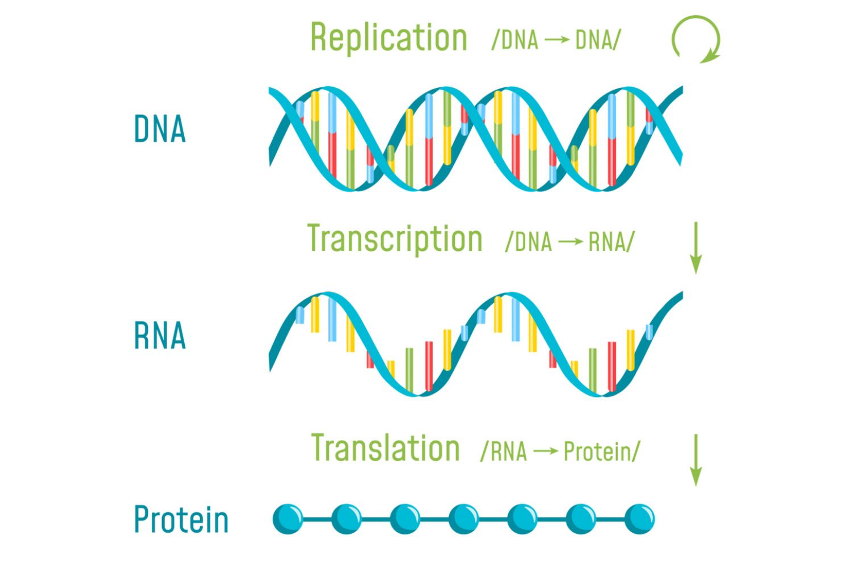
\includegraphics[width=0.5\linewidth]{\toplevelprefix/chapters/chapter1/figs/DNAs.png}
%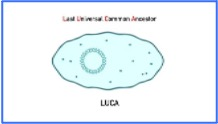
\includegraphics[width=0.28\linewidth]{\toplevelprefix/chapters/chapter1/figs/Luca.jpg}
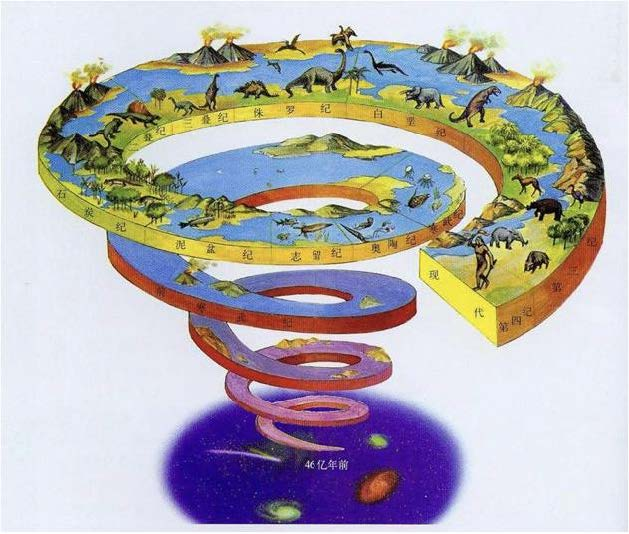
\includegraphics[width=0.40\linewidth]{\toplevelprefix/chapters/chapter1/figs/Evolution.jpg}
    \caption{物种进化智能的演化:外部世界的知识通过DNA(左图)编码和传递,并从DNA解码为RNA、蛋白质等。在生命演化的早期阶段(右图),智能通过(随机的)基因突变和自然选择——“适者生存”——在物种层面发展知识,这可以被看作是一种原始的强化学习形式。}
    \label{fig:phylogenetic}
\end{figure}
\begin{figure}
    \centering
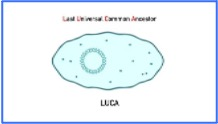
\includegraphics[height=0.19\linewidth]{\toplevelprefix/chapters/chapter1/figs/Luca.jpeg}
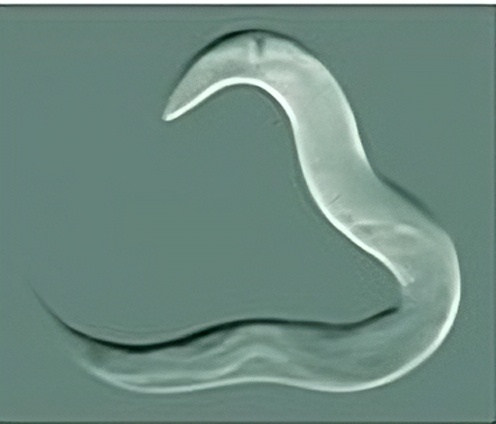
\includegraphics[height=0.19\linewidth]{\toplevelprefix/chapters/chapter1/figs/Worm.jpeg}
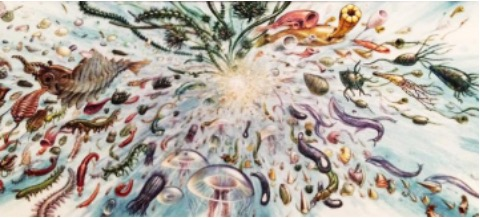
\includegraphics[height=0.19\linewidth]{\toplevelprefix/chapters/chapter1/figs/Cambrian.jpg}
    \caption{个体智能的演化,从今天所有生命的共同祖先(名为LUCA——最后普遍共同祖先),一个生活在35亿至43亿年前的单细胞样生物,到大约5.5亿年前蠕虫类物种(中图)中第一个神经系统的出现,再到大约5.3亿年前寒武纪时期(右图)生命形式的爆发。}
    \label{fig:evolution}
\end{figure}

{\em 个体智能}指的是允许个体在其特定的生活环境中,通过自己的感觉、记忆和预测进行学习,并改进和适应其行为的学习机制。个体智能在大约5.5亿至6亿年前神经系统出现后(在蠕虫样生物中)成为可能,如中图\ref{fig:evolution}所示。也就是说,有了感觉和神经系统,个体除了从其DNA或基因中继承的知识外,还能够不断形成和完善自己关于世界的知识,也称为记忆。这种能力显著增强了个体的生存能力,并促成了大约5.3亿年前寒武纪时期生命形式的爆发。与系统发育学习相比,个体发育学习效率更高、更可预测,可以在个体的生命周期内以有限的资源实现。

请注意,这两种学习机制都依赖于某种形式的反馈(来自外部环境),即对物种或个体的行为\footnote{物种的基因突变或个体做出的行为。}的惩罚(死亡)或奖励(食物)来进行学习。因此,所有智能生物,无论是作为物种还是作为个体,都依赖于一个闭环反馈机制来学习和完善它们关于世界的知识。我们还注意到,从植物到鱼类,再到鸟类和哺乳动物,更高级的物种越来越依赖于它们的个体学习能力。它们出生后与父母待在一起学习的时间越来越长,因为同一物种的个体需要在非常多样的环境中生存。

\paragraph{人类社会智能的演化。}
自大约31.5万年前智人出现以来,一种新的、更高级的智能形式出现了,它的演化更有效、更经济。语言,先是口头语言\footnote{据信梵语是第一种口头语言,可追溯到公元前5000年。},然后是书面语言\footnote{苏美尔语被认为是现存最古老的书面语言之一,最早可追溯到公元前约3100年的美索不达米亚南部。},在几千年前发展起来。参见图\ref{fig:human-intelligence}。这使得个体能够与他人交流和分享有用的信息。因此,一个人类社群或社会可以像一个单一的智能有机体一样行事,它能比任何个体学习得更快,拥有更多的知识。在某种程度上,书面语言或文本扮演着与DNA和基因相似的角色,因为它们允许人类社会积累关于世界的知识并将其传递给下一代。我们可以将这种智能称为{\em 社会智能},以区别于物种智能和个体智能。这种知识积累是古代文明出现与发展的基础。
\begin{figure}
    \centering
    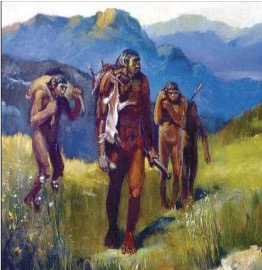
\includegraphics[height=0.25\linewidth]{\toplevelprefix/chapters/chapter1/figs/Spoken-language.jpg}
   \hspace{5mm} 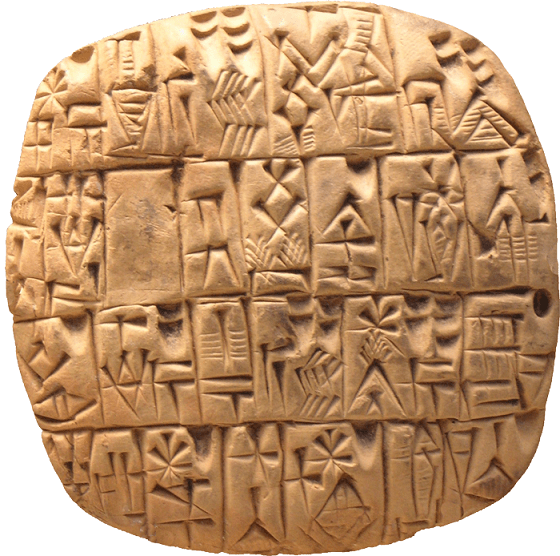
\includegraphics[height=0.25\linewidth]{\toplevelprefix/chapters/chapter1/figs/Cuneiform.png}
   \hspace{5mm} 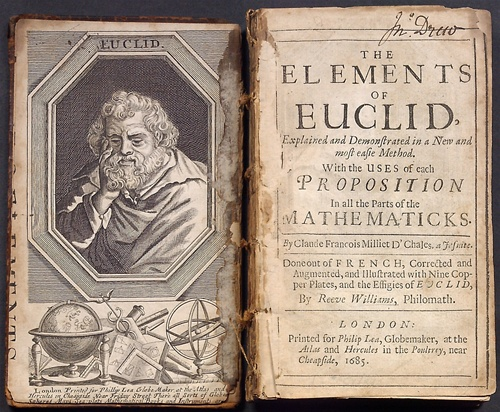
\includegraphics[height=0.25\linewidth]{\toplevelprefix/chapters/chapter1/figs/adopt-euclid1685-2.jpg}
    \caption{口头交流和口头语言(公元前10000-5000年)、书面语言(约公元前3000年)以及数学(约公元前500-300年)的发展,标志着人类智能演化中的三个关键里程碑。}
    \label{fig:human-intelligence}
\end{figure}

相当神奇的是,大约几千年前,人类智能发生了另一次量子飞跃,使得哲学家和数学家能够发展出似乎远超经验知识范畴的新知识。抽象数学概念和符号的发展,如数字、空间和时间,以及数理逻辑,成为现代科学的一种新的精确语言。此外,基于逻辑推导或科学实验来产生新假说并验证其正确性的能力也得到了发展。这首次使人类能够主动地发展新知识,超越了被动的经验手段。进行这些高级形式知识发展的能力被认为是人类所独有的。这种高级形式的智能被称为“人工智能”(AI),由约翰·麦卡锡在1956年达特茅斯夏季研讨会上创造。

因此,从我们能从自然界学到的东西来看,从现在起,每当我们使用“智能”这个词时,我们都需要非常具体地指明我们指的是哪个层次/形式的智能:
\begin{equation}
\mbox{\textbf{物种智能}} \;
   \Longrightarrow \; \mbox{\textbf{个体智能}} \; \Longrightarrow \; 
   \mbox{\textbf{社会智能}}
   \; \Longrightarrow \; 
   \mbox{\textbf{人工智能}}。
\end{equation}
清晰的刻画和区分是必要且重要的,因为我们希望将智能作为一个科学和数学的课题来研究。很有可能,即使它们都可能共享学习世界有用知识的共同目标,但每个层次/形式智能背后的具体计算机制和物理实现可能是不同的。我们相信,读者在读完本书后会更好地理解和欣赏这些差异。因此,我们将把更多的讨论留到最后一章,即第\ref{ch:future}章。


%Within the realm of biology, Lorenz and Tinbergen, who were pioneers in studying animal behavior (though not intelligence per se). In cognitive science, there is a long history, including behaviorists (reinforcement learning), Gestalt psychologists etc.

%Inspiration from Science. A biography of Norbert Wiener: ``Dark Hero of the Information Age: In Search Of Norbert Wiener--Father of Cybernetics'' by Conway and Siegelman. Connections to many biologists. Wiener studied zoology as a student.


\paragraph{机器智能的起源——控制论。}
在1940年代,部分由于战争的需要,自然界的智能启发了当时的科学家们用机器来模仿动物智能,这导致了由诺伯特·维纳倡导的“控制论”运动。维纳在哈佛大学本科时学习动物学,但后来成为一名数学家和控制理论家。维纳毕生热衷于理解和开发能够模仿动物智能行为的自主系统。今天,控制论项目常被人们狭隘地解释为主要是关于反馈控制系统,维纳确实在这方面做出了他最重要的技术贡献。但控制论项目远比这更广泛和深刻。它更多的是关于理解智能的整体\footnote{至少在动物的层面上。},并且实际上影响了一整代著名科学家的工作,包括沃伦·麦卡洛克、沃尔特·皮茨、克劳德·香农、约翰·冯·诺伊曼和艾伦·图灵。

\begin{figure}
    \centering
    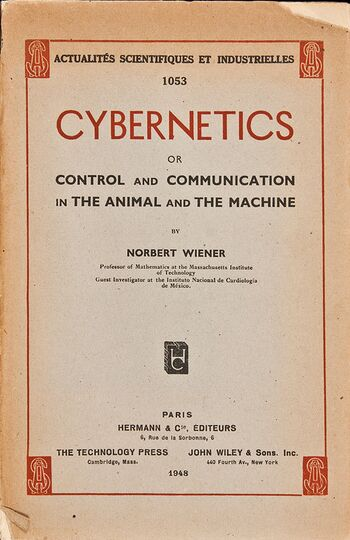
\includegraphics[height=0.4\linewidth]{\toplevelprefix/chapters/chapter1/figs/Cybernetics1.jpg}
    \hspace{10mm} 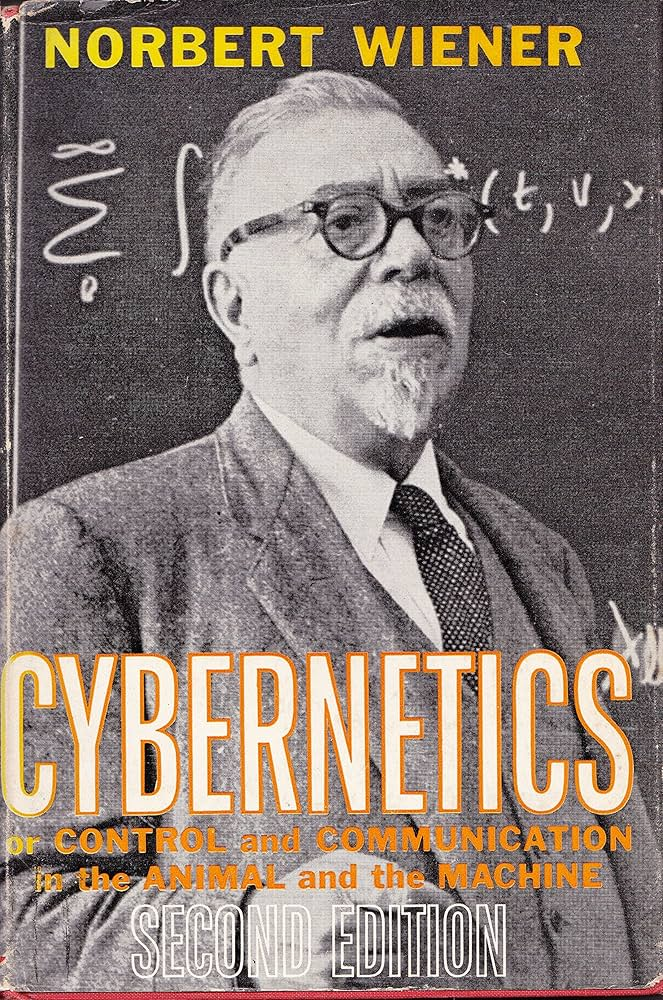
\includegraphics[height=0.4\linewidth]{\toplevelprefix/chapters/chapter1/figs/Cybernetics2.jpg}
    \caption{诺伯特·维纳于1948年出版的《控制论》一书 \cite{Wiener-Cybernetics-1948}(左)及其1961年的第二版 \cite{Wiener-Cybernetics-1961}(右)。}
    \label{fig:cybernetcis}
\end{figure}


维纳可以说是第一个将智能作为{\em 一个系统}来研究的人,而不仅仅是关注它的某个组成部分或方面。他对智能的全面看法在他著名的1948年著作《控制论:或关于在动物和机器中控制和通信的科学》\cite{Wiener-Cybernetics-1948}中得到了阐述。在这本书及其1961年出版的第二版中(见图\ref{fig:cybernetcis}),他试图确定智能系统的几个必要特征和机制,其中包括(但不限于):
\begin{itemize}
    \item 如何{\em 测量和存储}信息(在大脑中)以及如何与他人交流。\footnote{诺伯特·维纳是第一个指出“信息”既非物质也非能量,而是一个独立的研究量。} 这导致了克劳德·香农在1948年信息论和编码论的形成。
    \item 如何根据现有信息{\em 纠正}预测和估计中的错误。诺伯特·维纳本人在1940年代帮助形式化了基于闭环反馈的控制系统理论。
    \item 如何通过与潜在的非合作对手或对抗性环境互动来学习{\em 做出更好的决策}。这被约翰·冯·诺伊曼在1944年形式化为博弈论。
\end{itemize}
1943年,在维纳的控制论项目的极大推动下,精神病学家沃伦·麦卡洛克和逻辑学家沃尔特·皮茨共同形式化了第一个神经元的计算模型\cite{McCulloch-Pitts},称为{\em 人工神经元},后文图\ref{fig:neuron}将对此进行说明。基于这个模型,在1950年代,弗兰克·罗森布拉特建造了一台名为{\em Mark I 感知机}的物理机器,它由数百个这样的人工神经元网络组成。感知机是第一个物理实现的人工神经网络,见图\ref{fig:perceptron}。值得注意的是,约翰·冯·诺伊曼在1945年提出的通用计算机体系结构,其设计目的也是为了促进建造能够物理实现控制论项目所建议机制的{\em 计算机器}。

敏锐的读者可能已经注意到,1940年代确实是一个神奇的时代:许多基本思想被发明,许多有影响力的理论在那个时代被形式化,包括神经元的数学模型、人工神经网络、信息论、控制论、博弈论和计算机器。图\ref{fig:god-fathers}展示了这些理论的一些先驱。正如我们现在所知,上述每一项工作都已成长为后续几十年科学或工程领域的基础,并对我们产生了巨大影响。所有这些基本理论的灵感和动机都来自于开发能够模仿自然界智能的机器的目标。根据历史记载,维纳的控制论运动几乎影响了所有这些人及其工作。
\begin{figure}
    \centering
    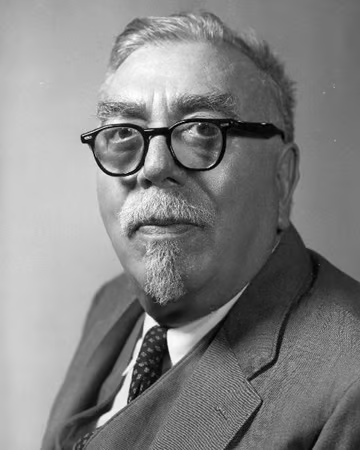
\includegraphics[height=0.3\linewidth]{\toplevelprefix/chapters/chapter1/figs/Wiener.png}
    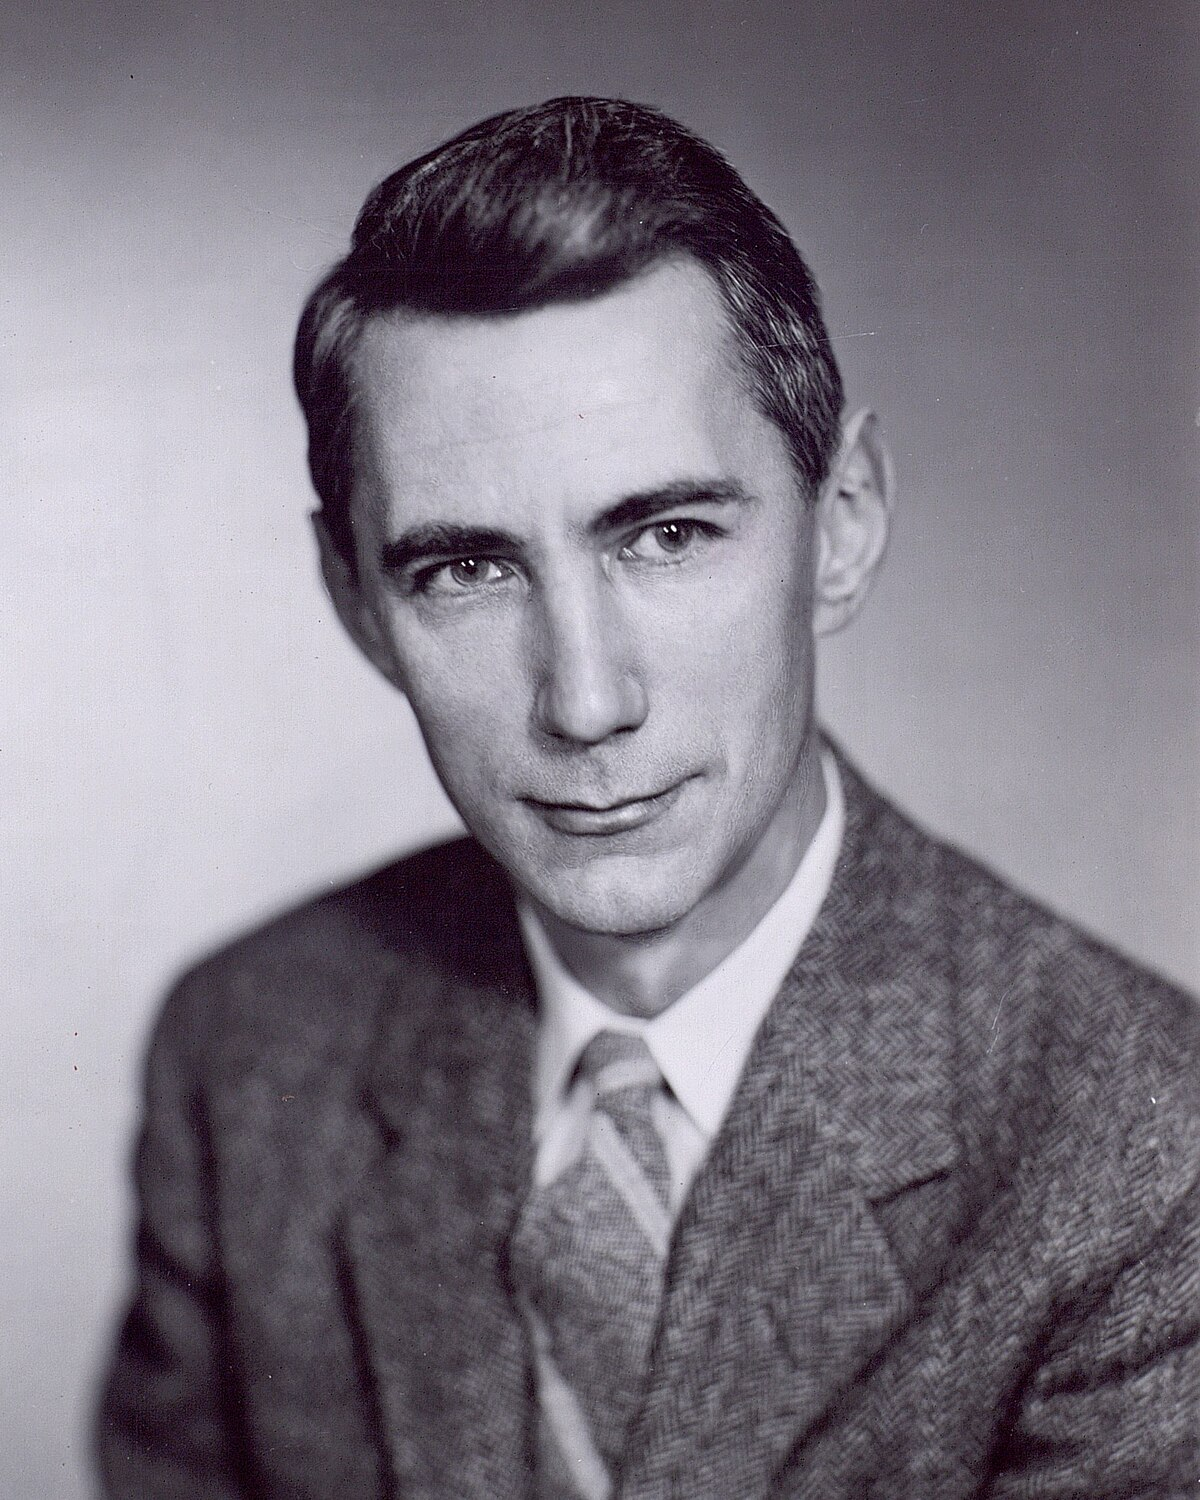
\includegraphics[height=0.3\linewidth]{\toplevelprefix/chapters/chapter1/figs/Shannon.jpg}
    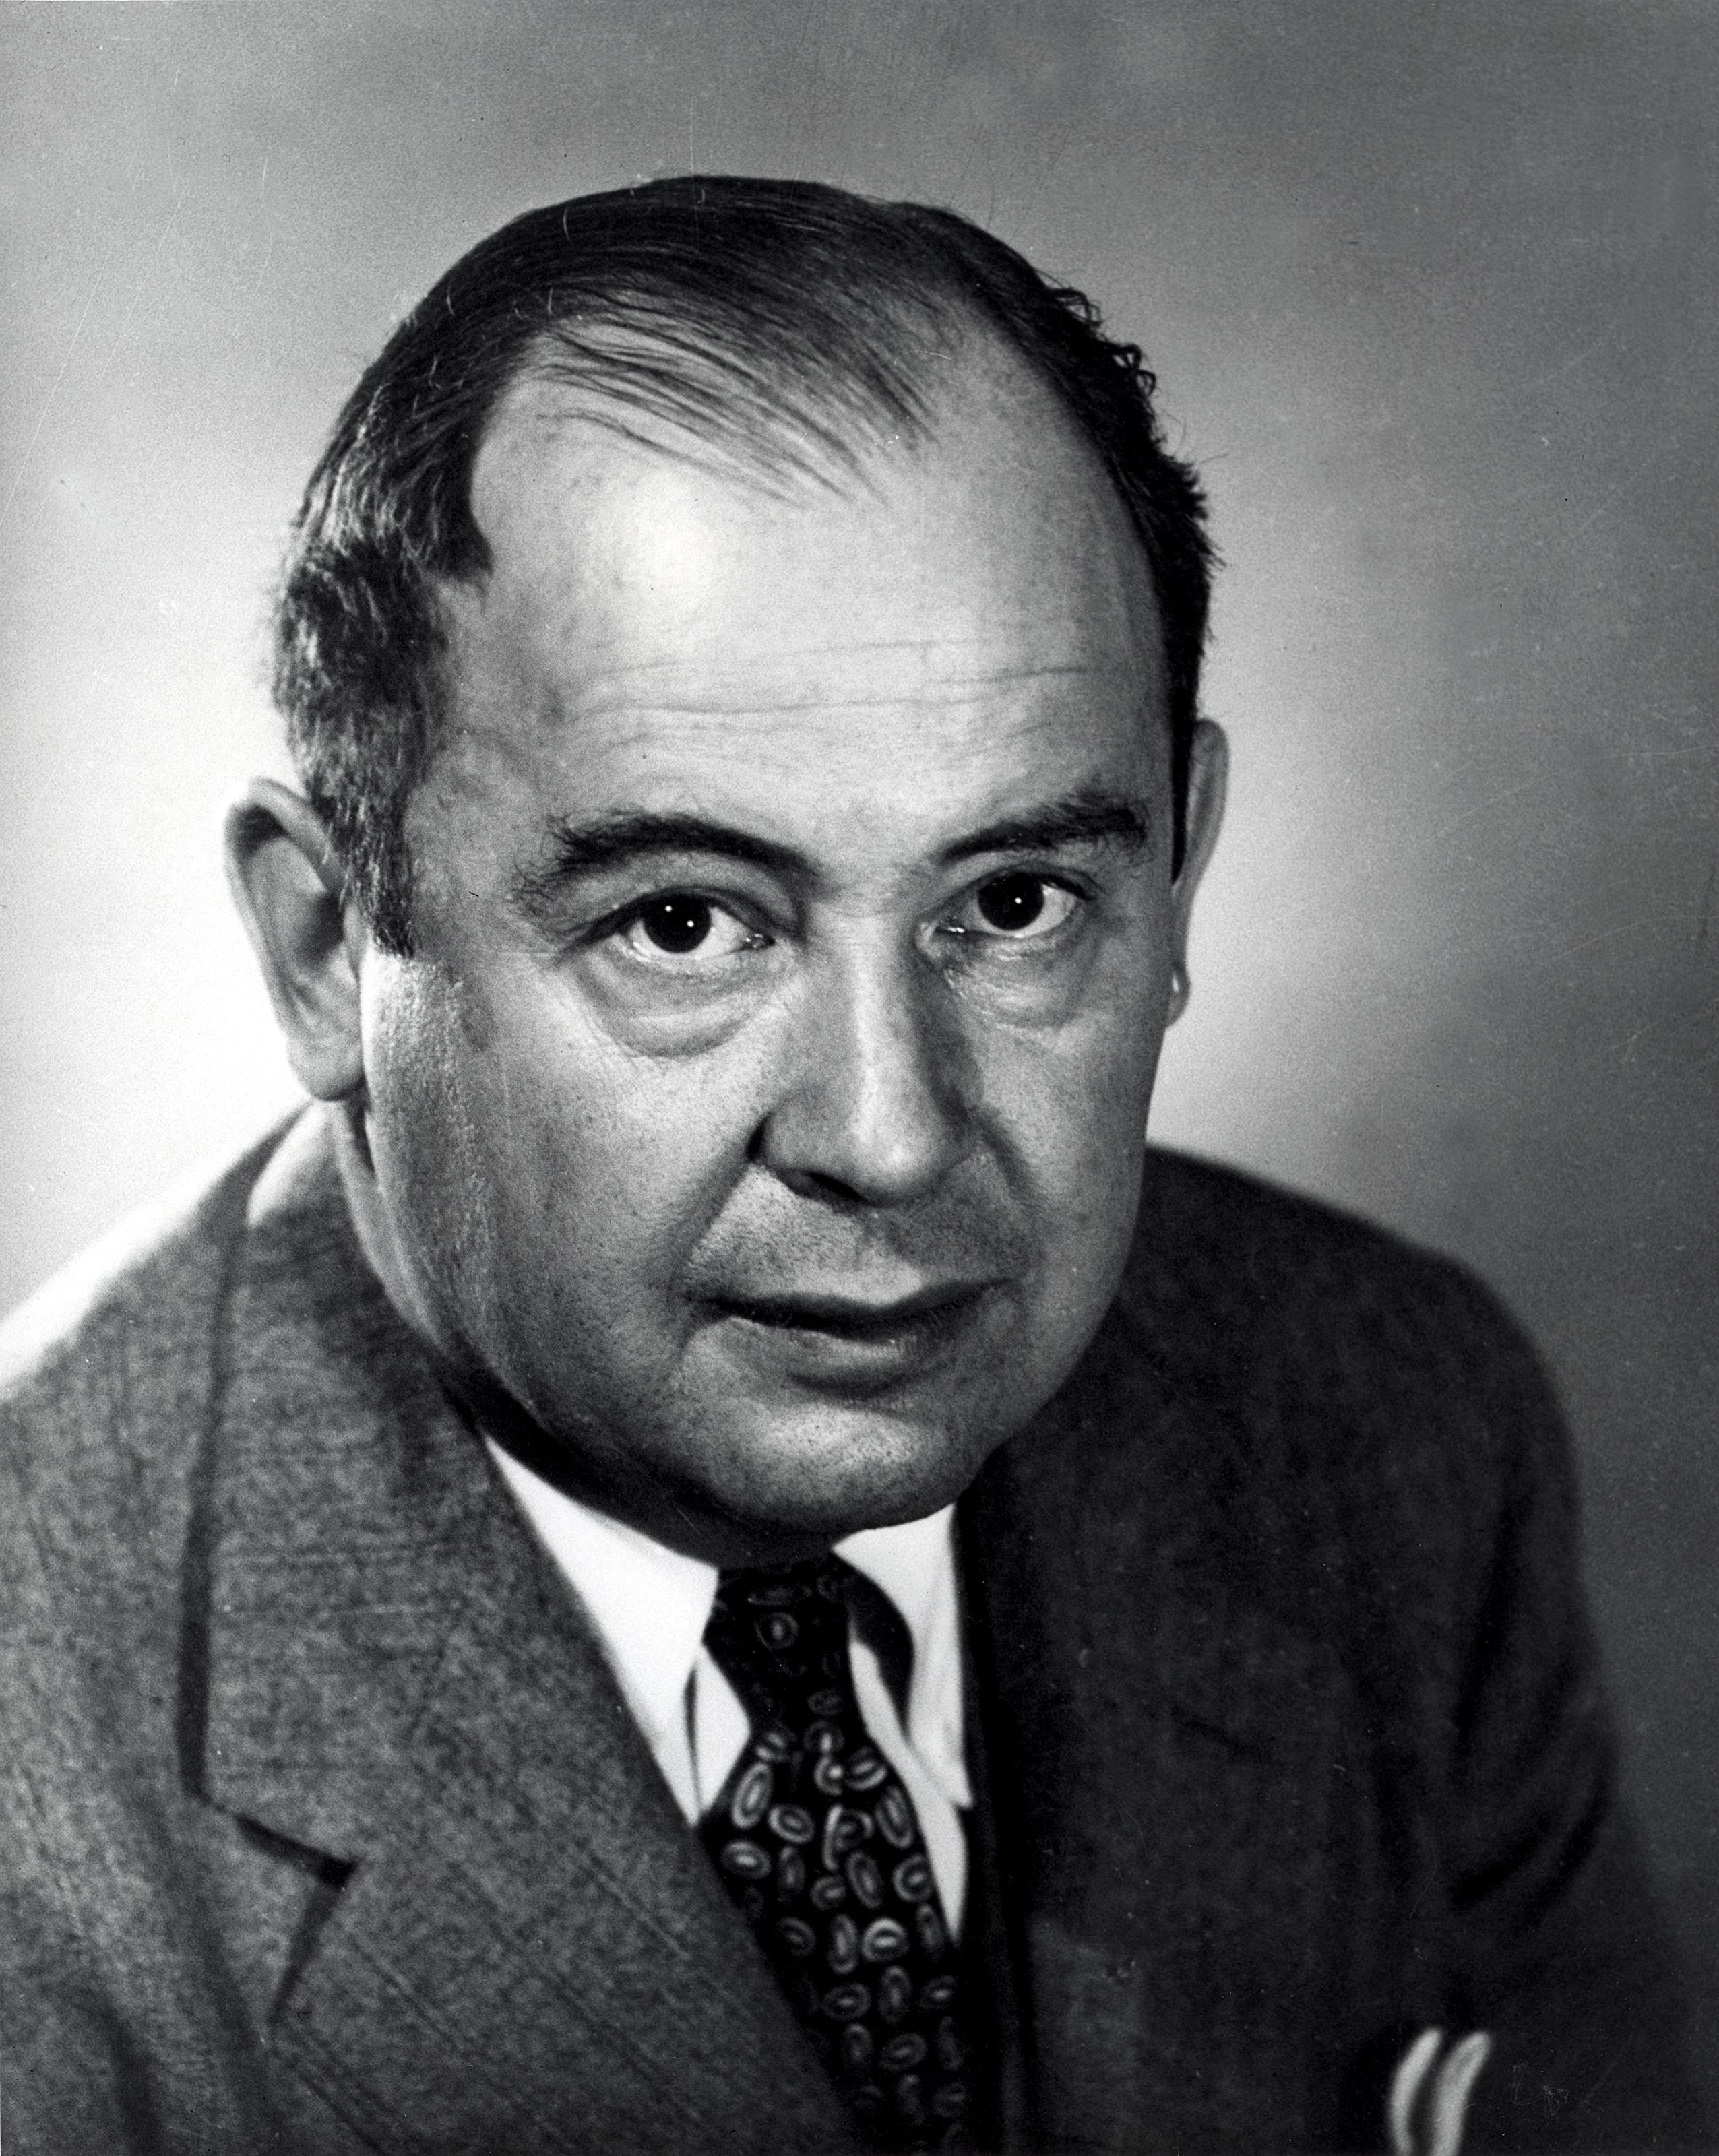
\includegraphics[height=0.3\linewidth]{\toplevelprefix/chapters/chapter1/figs/neumann.jpg}
    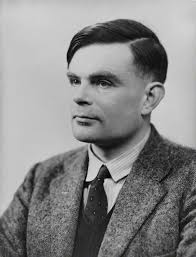
\includegraphics[height=0.3\linewidth]{\toplevelprefix/chapters/chapter1/figs/Turing.jpeg}
    \caption{智能的理论和计算基础的先驱:诺伯特·维纳(控制论和控制理论)、克劳德·香农(信息论)、约翰·冯·诺伊曼(博弈论)和艾伦·图灵(计算理论)。}
    \label{fig:god-fathers}
\end{figure}

尽管维纳在他的工作中指出了智能的许多关键特征和机制,但没有迹象表明他知道如何将所有这些机制恰当地整合在一起,以构建一个完整的自主智能系统。从今天的知识来看,他对这些机制的一些看法并不完全准确或完整。特别是在《控制论》第二版的最后一章\cite{Wiener-Cybernetics-1961}中,他指出,如果一个机器学习系统旨在模仿自然界中典型的学习机制,那么{\em 处理非线性}是至关重要的。但他没有为这个难题提供任何具体有效的解决方案。不过,这不能怪他。在当时,很少有人知道如何处理,因为即使是处理线性模型和系统的理论也还处于起步阶段。

尽管如此,我们不禁惊叹于维纳对非线性重要性的远见。正如我们将在本书中看到的,答案直到最近才被找到:非线性可以通过深度神经网络实现的渐进式线性化和变换来有效处理(见第\ref{ch:representation}章)。此外,我们将在本书中尝试展示如何将上述所有机制自然地整合到一个完整的系统中,该系统将展现出自主智能系统的特征(见第\ref{ch:autoencoding}章和第\ref{ch:closed-loop}章)。

\paragraph{人工智能的起源。}
从维纳的《控制论》一书的副标题:{\em “在动物和机器中的控制与通信”},可以看出1940年代的研究主要旨在模仿动物层面的智能。正如我们之前提到的,1940年代左右关于智能的研究议程在很大程度上由诺伯特·维纳的控制论运动主导。

艾伦·图灵是最早注意到这一局限性的人之一。在他著名的1950年论文《{\em 计算机器与智能}》\cite{Turing-1950}中,图灵正式提出了机器是否能模仿甚至达到人类水平的智能,以至于与人类的智能能力无法区分的问题。这现在被称为{\em 图灵测试}。

大约在1955年,一群年轻而雄心勃勃的科学家试图摆脱当时占主导地位的控制论运动和研究议程,以便他们有机会创造自己的遗产。他们决定接受图灵模仿人类智能的挑战,并提议于1956年夏天在达特茅斯学院举办一个研讨会。他们在提案中明确了他们的意图:
\begin{quote}
    “{\em 本研究将基于这样一个猜想进行:学习的每一个方面或智能的任何其他特征,原则上都可以被精确地描述,以至于可以制造一台机器来模拟它。我们将尝试找出如何让机器使用语言,形成抽象和概念,解决现在为人类保留的各种问题,并自我改进。}”
\end{quote}
实质上,他们希望形式化和研究区分人类与动物的高级智能。他们考虑的主题范围从抽象、符号方法、自然语言到演绎方法(包括因果推断、逻辑推导等)。研讨会的组织者,当时达特茅斯学院的年轻数学助理教授约翰·麦卡锡,创造了现在著名的术语“人工智能”(AI),以概括那些被认为是{\em 人类智能所独有}的特征或机制。

\paragraph{“人工智能”的复兴还是“控制论”的复兴?}
正如读者可能已经知道的,在过去十年左右的时间里,机器智能经历了爆炸性的发展,主要由深度人工神经网络的实践所驱动,这一浪潮由杰弗里·辛顿及其学生在2012年的工作\cite{krizhevsky2012imagenet}引发。这个时代也被誉为人工智能(AI)的“复兴”。然而,就人们实际尝试解决的任务(识别、生成和预测)以及人们迄今为止开发和实现的技术(强化、模仿、编码、解码、去噪和压缩)而言,我们很大程度上只是在模仿早期生命和动物智能中常见的机制。即便如此,正如我们将在本书中试图阐明的,当前的“AI”模型和系统尚未正确实现这些层面智能的所有必要机制,而这些机制在1940年代的控制论运动中就已经为人所知。

因此,严格来说,过去十年机器智能的进步与1956年达特茅斯研讨会所制定的“人工智能”计划并不十分吻合。相反,迄今为止主要完成的工作与诺伯特·维纳在1940年代制定的经典“控制论”计划的目标更为密切相关。或许称当前时代为“控制论的复兴”更为恰当。\footnote{最近兴起的所谓用于自主智能机器人的“具身AI”与控制论计划的目标有着更多的相似之处。} 只有在我们从科学和数学的角度充分理解了我们真正做了什么之后,我们才能真正知道还有什么需要做,以及应该朝哪个方向去追求智能的真正本质。这是本书的主要目的之一。


\section{学什么?}
\label{sec:what-to-learn}
%Notes: The notion of intelligence can be very  general and broad. But that often makes it ambiguous. Here, we here try to give a more precise description about what it mainly is. Our definition may have significantly narrowed the scope, but make it more implementable, verifiable, and even measurable (via computable means). 



\subsection{可预测性}
\label{sec:predictability}
携带有用信息的数据以多种不同形式表现出来。在最自然的形式中,它们可以被建模为可预测和可计算的序列。一个可预测和可计算序列的概念和性质是计算理论的核心,并在很大程度上导致了计算机的发明\cite{Turing-1936}。可预测序列在(归纳)推理中的作用在1960年代由雷·所罗门诺夫、安德雷·柯尔莫哥洛夫和许多其他人研究\cite{Kolmogorov1998OnTO},作为对克劳德·香农经典信息论\cite{Shannon-1948}的推广。为了理解可预测序列的概念,让我们首先从一些具体的简单例子开始。
\paragraph{标量情况。} 最简单的可预测离散序列可以说是自然数序列:
\begin{equation}
   {S} =  1, 2, 3, 4, 5, 6, \ldots, n, n+1, \ldots
\end{equation}
其中下一个数 $x_{n+1}$ 被定义为其前一个数 $x_n$ 加 1:
\begin{equation}
x_{n+1} = x_n + 1.    
\end{equation}
我们可以将可预测性的概念推广到任何序列 $\{x_n\}_{n=1}^\infty$(其中 $x_n \in \mathbb{R}$),如果下一个数 $x_{n+1}$ 总能从其前一个数 $x_n$ 计算得出:
\begin{equation}
    x_{n+1} = f(x_{n}), \quad x_n \in \mathbb{R}, \; n =  1, 2, 3, \ldots
\end{equation}
其中 $f(\cdot)$ 是一个{\em 可计算的}(标量)函数。\footnote{这里我们强调函数 $f(\cdot)$ 本身是可计算的,比如说它可以在计算机上作为程序实现。} 注意,这里我们强调函数 $f(\cdot)$ 必须是可计算的。有许多可以定义但不可计算的函数。艾伦·图灵在1936年的开创性工作\cite{Turing-1936}给出了可计算性的严格定义。在实践中,我们通常进一步假设 $f$ 是高效可计算的,并具有良好的性质,如连续和可微等。这些性质的必要性在我们对可计算性的更精细概念及其在机器学习和智能中的作用有了更多了解后会变得清晰。

\paragraph{多变量情况。}
当然,下一个数的值也可以依赖于它的两个前驱。例如,著名的{\em 斐波那契数列}定义为:
\begin{equation}
    {S} = 1, 1, 2, 3, 5, 8, 13, 21, 34, 55, \ldots
\end{equation}
其中可以很容易地看出:
\begin{equation}
    x_{n+2} = x_{n+1} + x_{n}, \quad  x_n \in \mathbb{R}, \;  n = 1, 2, 3, \ldots
\end{equation}
类似地,我们可以将这个递归推广到 \begin{equation}
    x_{n+2} = f(x_{n+1}, x_{n}), \quad x_n \in \mathbb{R}, \;  n =  1, 2, 3, \ldots
\end{equation}
其中 $f(\cdot,\cdot)$ 是任何以两个变量为输入的可计算函数。我们可以进一步将可预测性的概念推广到一个序列,其下一个值依赖于它的 $d$ 个前驱:
\begin{equation}
    x_{n+d} = f(x_{n+d-1}, \ldots,  x_{n}), \quad  x_n \in \mathbb{R}, \; n =  1, 2, 3, \ldots
    \label{eqn:recursive-d}
\end{equation}
预测所需的前驱数量 $d$ 被称为递归预测的{\em 阶数}。上述表达式\eqref{eqn:recursive-d}也称为{\em (自)回归}。这样的序列也称为{\em 自回归}序列。如果函数 $f$ 是一个线性函数,我们称之为线性(自)回归。

\paragraph{向量情况。} 
为了简化符号,我们可以定义一个向量 $\vx \in \mathbb{R}^d$,它收集了序列中 $d$ 个连续的值 \begin{equation}
    \vx_n \doteq [x_{n+d-1}, \ldots,  x_{n}]^\top, \quad \vx_n \in \mathbb{R}^d, \; n = 1, 2, 3, \ldots
\end{equation}
使用这个符号,递归关系\eqref{eqn:recursive-d}可以方便地写成
\begin{equation}
    \vx_{n+1} = g(\vx_{n}) \; \in \mathbb{R}^d, \quad n =  1, 2, 3, \ldots
    \label{eqn:recursive-v}
\end{equation}
其中函数 $g(\cdot)$ 由\eqref{eqn:recursive-d}中的函数 $f$ 唯一确定,它以一个 $d$ 维向量为输入。在不同的上下文中,这样的向量有时被称为“状态”或“令牌”(token)。注意,\eqref{eqn:recursive-d}中的方程表示一个映射 $\mathbb{R}^d \rightarrow \mathbb{R}$,但这里的方程是 $g: \mathbb{R}^d \rightarrow \mathbb{R}^d$。


\paragraph{受控预测。}
我们也可以定义一个依赖于另一个可预测序列作为输入的可预测序列:
\begin{equation}
    \vx_{n+1} = f(\vx_{n}, \vu_n) \; \in \mathbb{R}^d, \quad n =  1, 2, 3, \ldots,
\label{eqn:recursive-control}
\end{equation}
其中 $\{\vu_n\}$($\vu_n \in \mathbb{R}^k$)是一个(可计算的)可预测序列。换句话说,下一个向量 $\vx_{n+1} \in \mathbb{R}^d$ 依赖于 $\vx_n \in \mathbb{R}^d$ 和 $\vu_n \in \mathbb{R}^k$。在控制理论的背景下,序列 $\{\vu_n\}$ 通常被称为“控制输入”,而 $\vx_n$ 被称为系统\eqref{eqn:recursive-control}的“状态”或“输出”。一个经典的例子是线性动力系统:
\begin{equation}
    \vx_{n+1} = \boldsymbol{A}\vx_n + \boldsymbol{B}\vu_n, \quad \boldsymbol{A} \in \mathbb{R}^{d\times d}, \boldsymbol{B} \in \mathbb{R}^{d\times k},
    \label{eqn:lineary-system} 
\end{equation}
这在控制理论中被广泛研究\cite{Cal:Des}。

很多时候,控制输入由状态 $\vx_n$ 本身的一个可计算函数给出,比如说:
\begin{equation}
    \vu_n = h(\vx_n), \quad n =  1, 2, 3, \ldots 
\end{equation}
因此,序列 $\{\vx_n\}$ 由两个可计算函数 $f$ 和 $h$ 的复合给出:
\begin{equation}
    \vx_{n+1} = f\big(\vx_{n}, h(\vx_n)\big), \quad n =  1, 2, 3, \ldots
    \label{eqn:recursive-closed-loop}
\end{equation}
这样,序列 $\{\vx_n\}$ 再次成为一个自回归的可预测序列。当输入 $\vu_n$ 依赖于输出 $\vx_n$ 时,我们说所得到的序列是由一个“闭环”系统\eqref{eqn:recursive-closed-loop}产生的。由于闭环系统不再依赖于任何外部输入,我们说这样的系统已经变得{\em 自主的}。它可以被看作是自回归的一个特例。例如,如果我们在上述线性系统\eqref{eqn:lineary-system}中选择 $\vu_n = \boldsymbol{F}\vx_n$,闭环系统就变成
\begin{equation}
        \vx_{n+1} = \boldsymbol{A}\vx_n + \boldsymbol{B}\vu_n = \boldsymbol{A}\vx_n + \boldsymbol{B}\boldsymbol{F}\vx_n = (\boldsymbol{A}+ \boldsymbol{B}\boldsymbol{F})\vx_n,
    \label{eqn:lineary-system-closed}
\end{equation}
这是一个线性自回归。

% \paragraph{Approximate prediction.}
% What if in the above equation \eqref{eqn:recursive-control} the input sequence $\vu_n$ is not predictable? One extreme case is when it is completely unpredictable, say:
% \begin{equation}
%     \vx_{n+1} = f(\vx_{n}, \boldsymbol{\epsilon}_n), \quad n =  1, 2, 3, \ldots
%     \label{eqn:recursive-noise}
% \end{equation}
% where $\boldsymbol{\epsilon}_n \in \mathbb{R}^k$ is some random (Gaussian) noise. In such cases, we say the so-defined sequence $\{\vx_n\}$ ``stochastic''. Obviously, such a sequence is no longer fully predictable, at least not in a deterministic sense as above. 

% When magnitude of the noise  $\|\boldsymbol{\epsilon}_n\|$ is small and the function $f$ does not amplify the noise so much, we have
% \begin{equation}
%     \vx_{n+1} \approx f(\vx_{n}, \boldsymbol{0}) + \nabla_{\boldsymbol{\epsilon}}f(\vx_{n}, \boldsymbol{0})   \boldsymbol{\epsilon}_n, \quad n =  1, 2, 3, \ldots
%     \label{eqn:recursive-noise-small}
% \end{equation}
% where the magnitude of the second term $\|\nabla_{\boldsymbol{\epsilon}}f(\vx_{n}, \boldsymbol{0})   \boldsymbol{\epsilon}_n\|$ is small. Hence $ \vx_{n+1}$ is largely determined by the first deterministic term and its expectation is predictable: 
% \begin{equation}
%     \mathbb{E}[\vx_{n+1}] \approx f(\vx_{n}, \boldsymbol{0}).
% \end{equation}
% In this case, we say the sequence $\{\vx_n\}$ defined by \eqref{eqn:recursive-noise-small} is ``approximately predictable''. In practice, we often deal with this type of approximate predictability in real-world data in which  measurement noises are commonplace. Note that taking the expectation essentially removes the effect of  random noise and renders the expectation $\{\mathbb{E}[\vx_n]\}$ a predictable sequence. Such a process is typically referred to as ``denoising''. \DP{the connection between ``denoising'' here and ``denoising'' in Ch 2/3 is not obvious at first glance. For instance, here it is w.r.t.~an autoregressive sequence, but later it is for single observations. this isn't the same thing as filtering either. I don't really see why we need this paragraph (at least here).} 

\paragraph{连续过程。}
可预测序列在连续情况下有其自然的对应物。我们可以称它们为可预测过程。与自然数序列类似,最简单的可预测连续过程是时间本身 $x=t$。

更一般地,我们说一个过程,记为 $\vx(t)$,是可预测的,如果在任何时间 $t$,该过程在 $t+\delta t$ 的值(其中 $\delta t$ 是一个无穷小增量)由其在 $t$ 的值确定。通常,值的变化 $\delta \vx(t)$ 是连续和平滑的。所以 $\delta \vx(t) = \vx(t + \delta t) - \vx(t)$ 是无穷小的。可预测过程通常由(多变量)微分方程描述:
\begin{equation}
    \dot{\vx}(t) = f(\vx(t)), \quad \vx \in \mathbb{R}^d. 
    \label{eqn:process}
\end{equation}

在系统理论的背景下\cite{Cal:Des,Sastry-Nonlinear},上述方程也称为状态空间模型。与离散情况类似,一个受控过程可以由以下公式给出:
\begin{equation}
    \dot{\vx}(t) = f(\vx(t), \vu(t) ), \quad \vx \in \mathbb{R}^d, \vu \in \mathbb{R}^k,
    \label{eqn:process-controlled}
\end{equation}
其中 $\vu(t)$ 是一个可计算的输入过程。

\begin{example}
    例如在物理学中,牛顿第二运动定律描述了如何预测一个运动物体在力输入 $\boldsymbol{F}(t) \in \mathbb{R}^3$ 下的轨迹 $\boldsymbol{x}(t) \in \mathbb{R}^3$:
\begin{equation}
    m\ddot{\boldsymbol{x}}(t) = \boldsymbol{F}(t).
\end{equation}
当没有力 $\boldsymbol{F}(t) \equiv 0$ 时,上述定律简化为一个特例,即牛顿第一定律:物体以恒定速度沿直线运动:
\begin{equation}
   \ddot{\boldsymbol{x}}(t) = \boldsymbol{0} \; \Leftrightarrow \; \dot{\boldsymbol{x}}(t) = \boldsymbol{v}
\end{equation}
其中 $\boldsymbol{v} \in \mathbb{R}^3$ 是某个恒定的速度向量。
\end{example}




\subsection{低维性}\label{sec:intro-low-dimensionality}
\paragraph{学习去预测。}
现在假设你已经观察到或被给予了许多序列片段:
\begin{equation}
    \{S_1, S_2, \ldots, S_i, \ldots, S_N\}
\end{equation}
它们都来自某个可预测序列 $\{x_n\}_{n=1}^\infty$。不失一般性,我们可以假设每个片段的长度为 $D \gg d$。所以每个片段的形式为:
\begin{equation}
    S_i = [x_{j(i)}, x_{j(i)+1}, \ldots, x_{j(i)+D-1}]^\top \in \mathbb{R}^D
\end{equation}
对于某个 $j \in \mathbb{N}$。然后你被给予一个新的片段 $S_t$,并被要求预测其未来的值。

这里的一个困难是,你通常不知道生成该序列的函数 $f$ 和阶数 $d$:
\begin{equation}
    x_{n+d} = f(x_{n+d-1}, \ldots,  x_{n}).
\label{eqn:sequence-order-d}
\end{equation}
所以希望是能以某种方式从给定的样本片段 $S_1, S_2, \ldots, S_N$ 中“学习”到 $f$ 和 $d$。因此,学习预测的核心任务是:
\begin{center}
{\em 给定一个可预测序列的许多采样片段,如何有效且高效地辨识函数 $f$。}
\end{center}

\paragraph{可预测性与低维性。}
为了辨识预测函数 $f$,我们可能会注意到任何可预测序列(比如由\eqref{eqn:sequence-order-d}给出的序列)的片段的一个共同特征。如果我们取一个长片段,比如说长度为 $D \gg d$ 的序列,并将其视为一个向量:
\begin{equation}
    \vx_i = [x_i, x_{i+1}, \ldots x_{i+D-1}]^\top \in \mathbb{R}^D.
\end{equation}
那么所有这些向量的集合 $\{\vx_i\}$ 远非随机,因此不可能占据整个 $\R^D$ 空间。相反,它们本质上最多有 $d$ 个自由度——给定任何 $\vx_i$ 的前 $d$ 个条目,其余条目的值是唯一确定的。换句话说,所有的 $\{\vx_i\}$ 都位于一个 $d$ 维的曲面上。在数学中,这样的曲面通常被称为子流形,记为 $\mathcal{S} \subset \R^D$。


\begin{figure}[t]
\centering
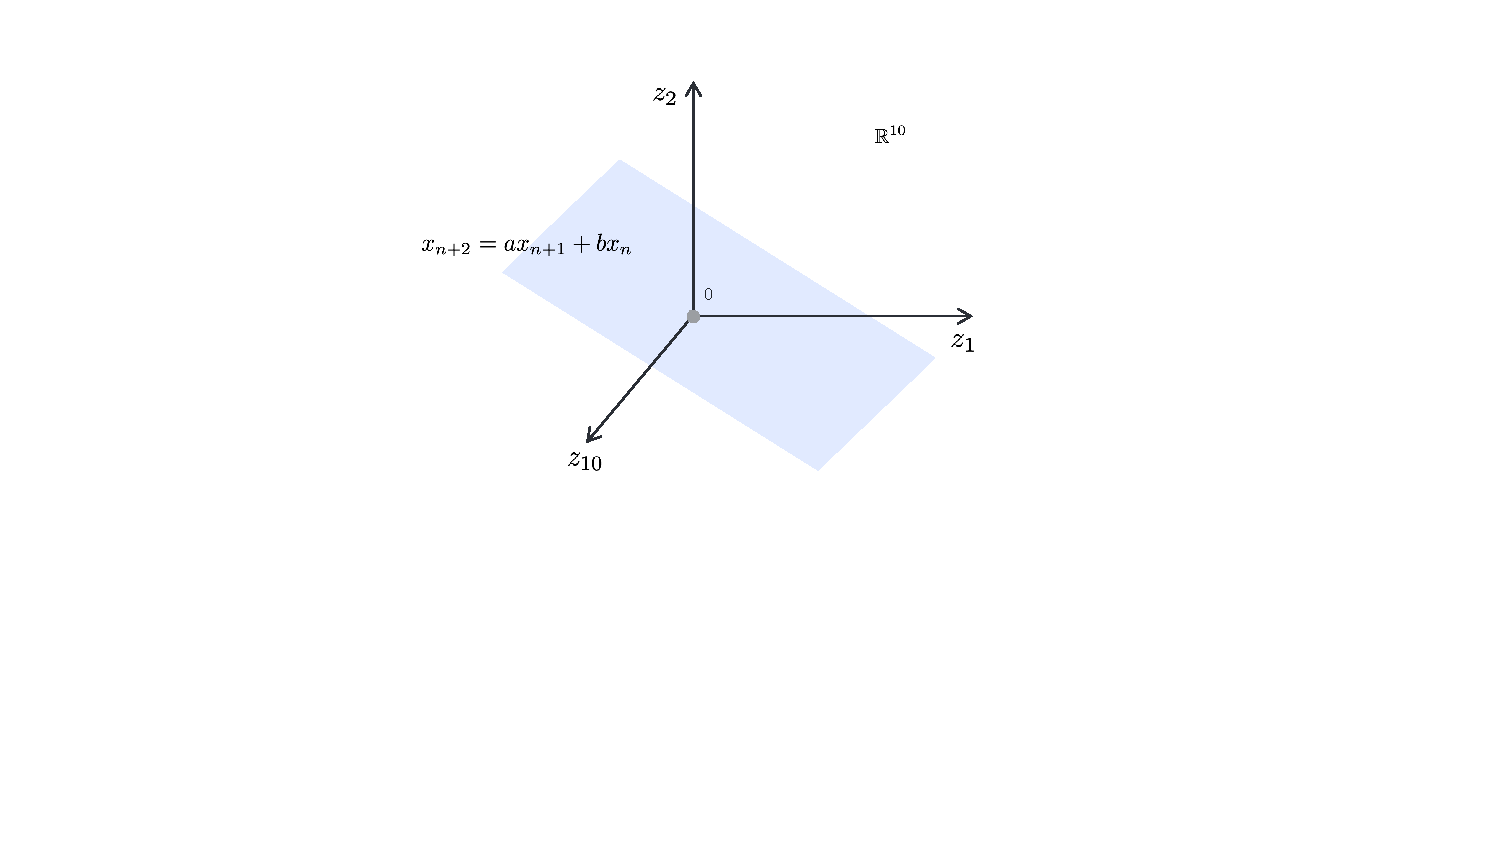
\includegraphics[width=0.6\linewidth]{\toplevelprefix/chapters/chapter1/figs/two-dimensional plane in R10.pdf}
    \caption{一个十维环境空间中的二维子空间。}
    \label{fig:lowdimplane}
\end{figure}
在实践中,如果我们选择足够大的片段长度 $D$,那么从同一个预测函数采样的所有片段都位于一个内在维度为 $d$ 的曲面上,这个维度远低于环境空间 $D$ 的维度。例如,如果序列由以下线性自回归给出:
\begin{equation}
    x_{n+2} = a\cdot x_{n+1} + b\cdot x_n,
    \label{eqn:sequence-2d}
\end{equation}
对于某些常数 $a, b \in \R$。如果我们从这样的序列中采样长度为 $D=10$ 的片段,那么所有样本都位于 $\R^{10}$ 中的一个二维平面或子空间上,如图\ref{fig:lowdimplane}所示。如果我们能辨识出这个二维子空间,那么\eqref{eqn:sequence-2d}中的常数 $a$ 和 $b$ 就可以完全确定。


很容易看出,如果预测函数 $f$ 是线性的,例如在\eqref{eqn:lineary-system}和\eqref{eqn:lineary-system-closed}中给出的线性系统,长片段总是位于某个低维线性子空间上。辨识预测函数在很大程度上等同于辨识这个低维子空间,这个问题通常被称为主成分分析。我们将在第\ref{ch:classic}章讨论这些经典模型和方法。

事实证明,对于一般的可预测序列,这在很大程度上也是成立的:如果能够辨识出所有片段样本所在的低维曲面,那么就可以辨识出相关的预测函数 $f$。\footnote{在温和的条件下,低维曲面和函数 $f$ 之间存在一一映射。这一事实在诸如系统辨识等问题中得到了利用,我们稍后会讨论。} 我们不能过分强调可预测序列片段的这一性质的重要性:{\em 一个可预测序列的所有长片段样本都位于一个低维子流形上。} 正如我们将在本书中看到的,所有现代学习方法,无论是隐式还是显式,都利用了这一性质。%\yima{Add a Figure to illustrate the surface or submanifold.} 

在现实世界的情景中,我们观察到的数据通常不来自单个可预测序列。它们通常包含对多个可预测序列的观察。例如,一个视频序列可以包含多个移动的物体。很容易看出,在这种情景下,数据位于多个低维线性子空间或非线性子流形的混合体上,如图\ref{fig:mixture-models}所示。
\begin{figure}
    \centering
    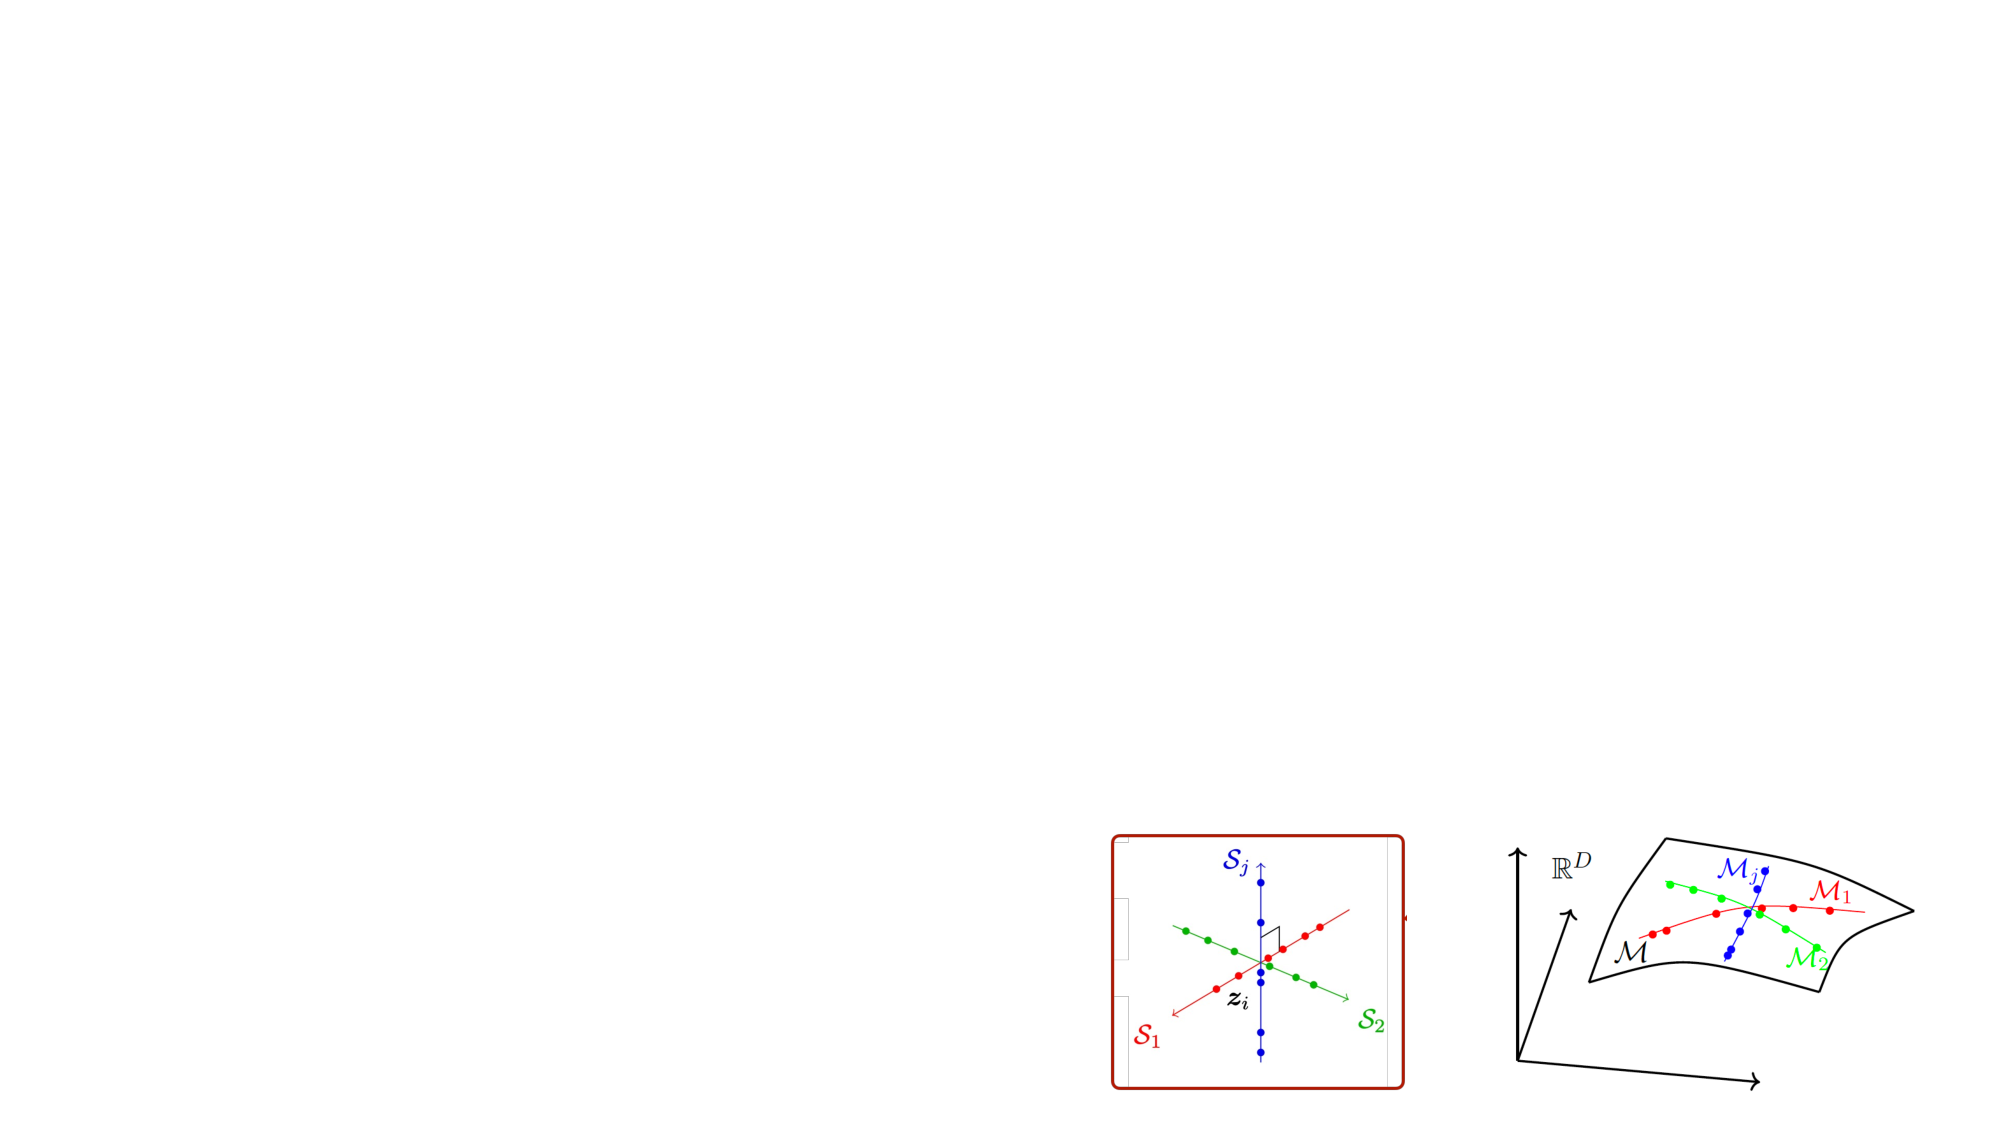
\includegraphics[width=0.8\linewidth]{\toplevelprefix/chapters/chapter1/figs/mixture.pdf}
    \caption{分布在(正交)子空间(左)或子流形(右)混合体上的数据。}
    \label{fig:mixture-models}
\end{figure}


\paragraph{低维性的性质。}
当然,可预测序列中的时间相关性并不是数据低维的唯一原因。例如,所有图像的空间是巨大的,但大部分空间由类似于图\ref{fig:noise-image}左侧所示的无结构随机图像组成。然而,自然图像和视频是高度冗余的,因为所有像素值之间存在强烈的空间和时间相关性。这就是为什么我们可以轻易地识别出一张图像是噪声图像还是清晰图像,如图\ref{fig:noise-image}中图和右图所示。因此,自然图像的分布具有非常低的内在维度(相对于图像的总像素数)。

\begin{figure}
    \centering
    
\includegraphics[height=0.30\linewidth]{\toplevelprefix/chapters/chapter1/figs/Gaussian-noise.png}\hspace{2mm} 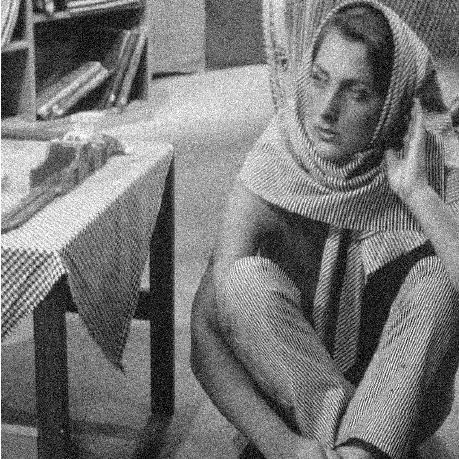
\includegraphics[height=0.30\linewidth]{\toplevelprefix/chapters/chapter1/figs/Standard-test-image-Barbara-of-size-512-512-pixels-including-Gaussian-noise-with.png} \hspace{2mm} 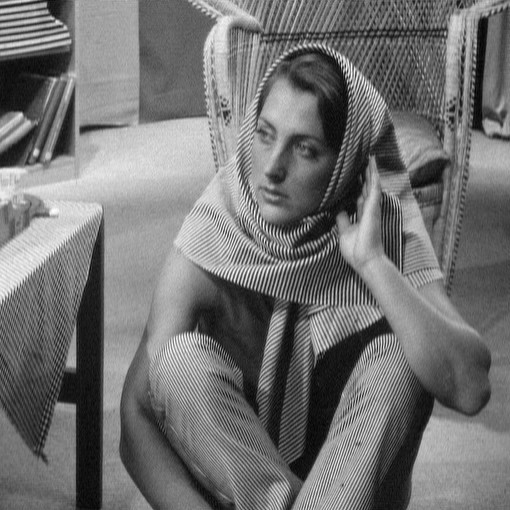
\includegraphics[height=0.30\linewidth]{\toplevelprefix/chapters/chapter1/figs/barbara.jpg}
    \caption{一张随机噪声图像与一张带噪图像以及原始清晰图像的对比。%\sdb{probably want to avoid using Lena given all the IEEE/PAMI-TC/etc.\ recent motions}
    }
    \label{fig:noise-image}
\end{figure}

由于学习低维结构任务的重要性和普遍性,《高维数据分析与低维模型:原理、计算与应用》\cite{Wright-Ma-2022}一书在开头就指出:“{\em 在高维空间中辨识信号或数据的低维结构问题,是贯穿系统理论、信号处理、模式识别、机器学习和统计学等众多工程和数学领域悠久历史的最基本问题之一。}”

请注意,通过强制观测数据点 $\vx$ 位于一个低维曲面上,我们实际上已经使 $\vx$ 的各个条目之间高度相关,在某种意义上使这些条目可以从其他条目的值中“预测”出来。例如,如果我们知道数据被约束在 $\R^D$ 中的一个 $d$ 维曲面上,那么除了预测之外,我们还可以对数据做许多有用的事情:%\yima{Maybe some illustrations for these properties.}
\begin{itemize}
    \item \textbf{补全}:一般来说,给定一个典型样本 $\vx$ 的超过 $d$ 个条目,其余的条目通常可以被{\em 唯一}确定。\footnote{预测成为这个性质的一个特例。}
    \item \textbf{去噪}:假设一个样本 $\vx$ 的条目被{\em 小}噪声扰动,可以通过将 $\vx$ 投影回曲面上来有效地去除它们。
    \item \textbf{纠错}:假设 $\vx$ 的少数{\em 未知}条目被任意损坏,它们可以被有效且高效地纠正。
\end{itemize}
图\ref{fig:low-dim-properties}用一个低维线性结构——二维平面中的一维直线——来说明这些性质。

\begin{figure}
    \centering
    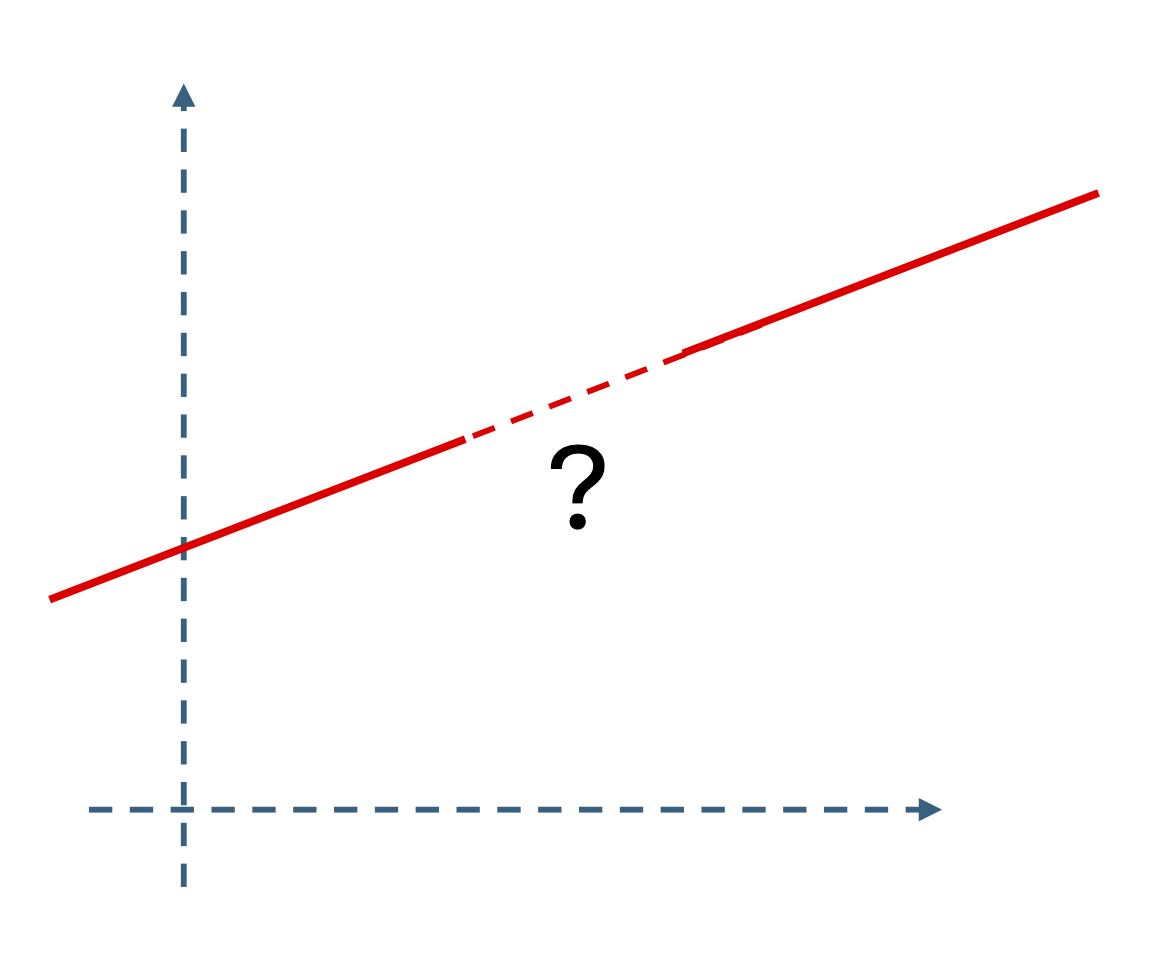
\includegraphics[height=0.28\linewidth]{\toplevelprefix/chapters/chapter1/figs/Completion-low-dim.png}     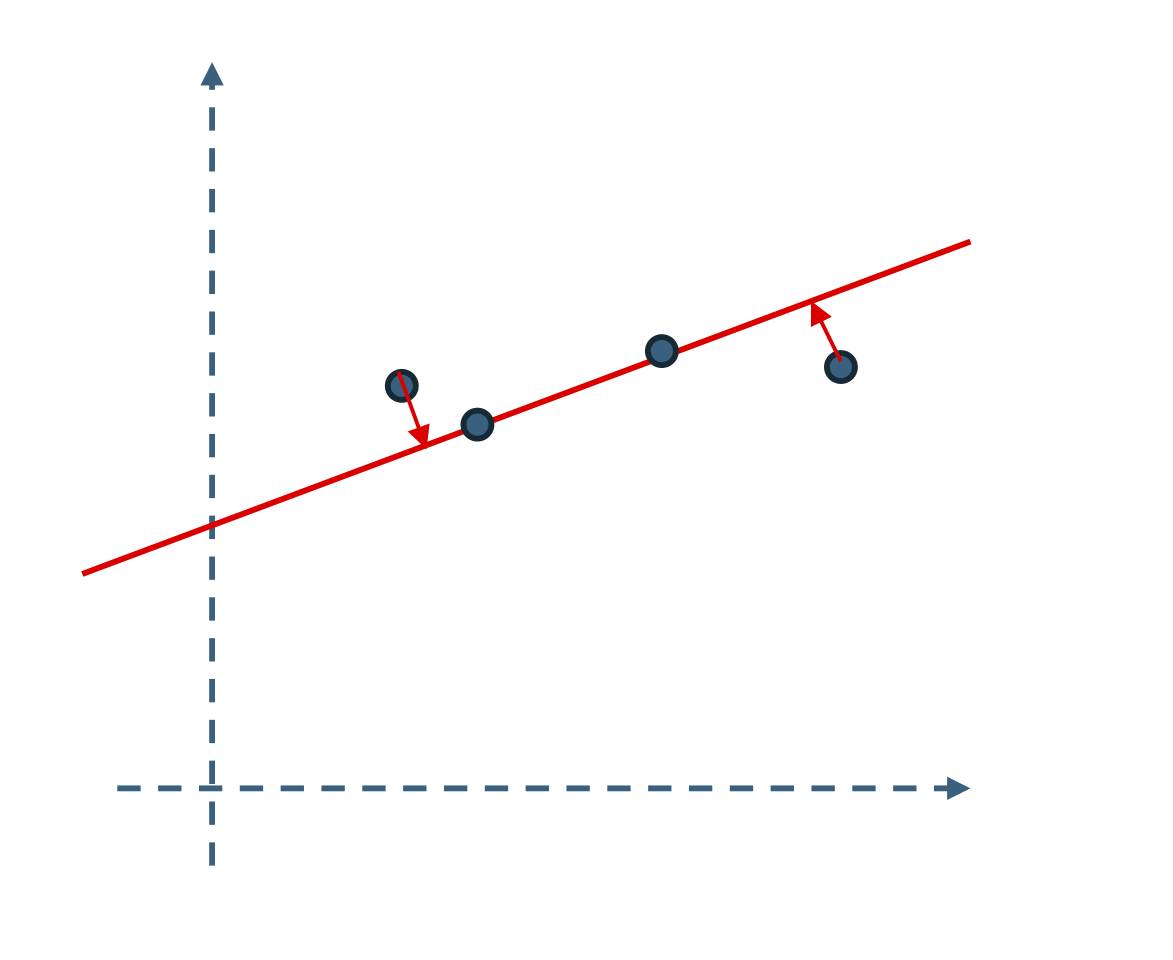
\includegraphics[height=0.28\linewidth]{\toplevelprefix/chapters/chapter1/figs/Denoising-low-dim.png} 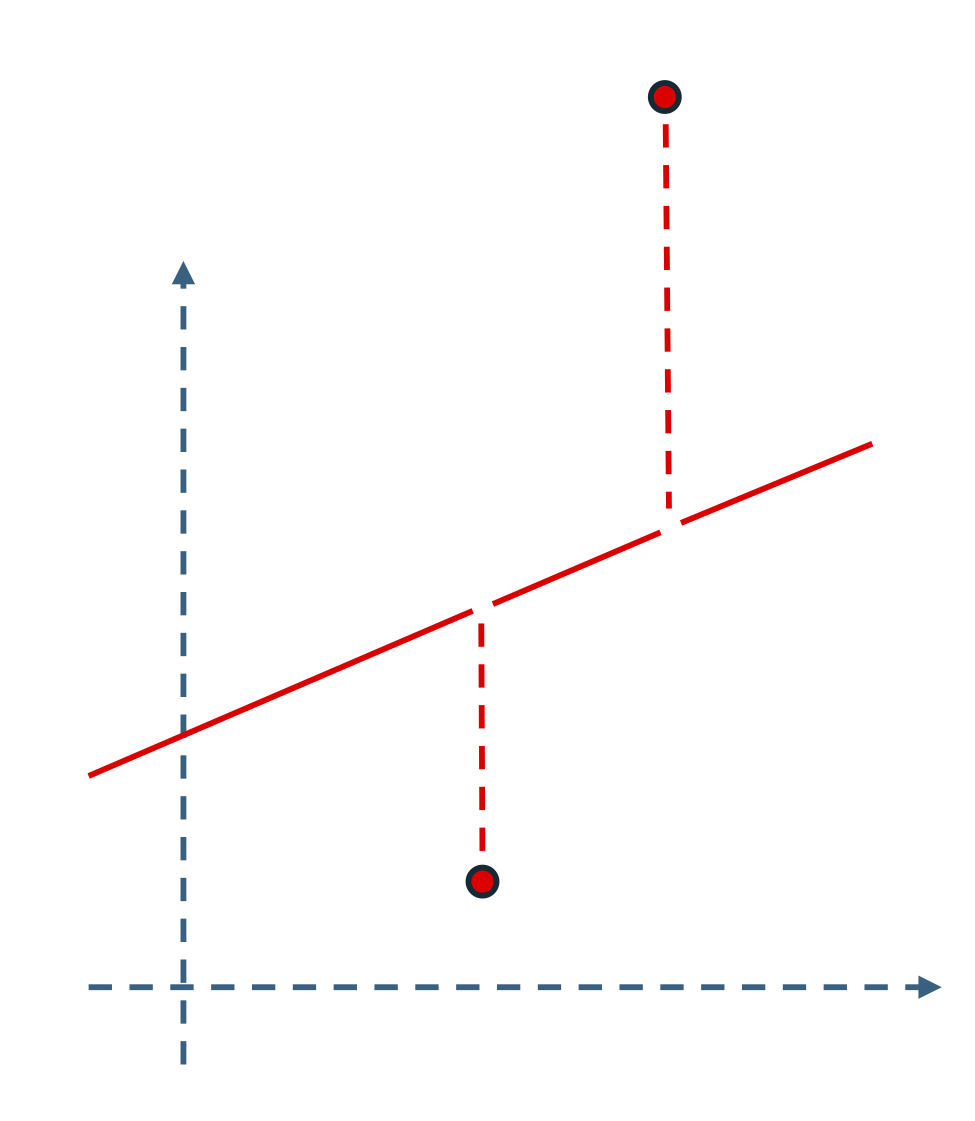
\includegraphics[height=0.32\linewidth]{\toplevelprefix/chapters/chapter1/figs/Correction-low-dim.png} 
    \caption{低维(线性)结构性质的图示:它支持补全(左)、去噪(中)和纠错(右)。}
    \label{fig:low-dim-properties}
\end{figure}

事实上,在温和的条件下,上述性质可以推广到高维空间中的许多其他低维结构\cite{Wright-Ma-2022}。有趣的是,正如我们将在本书中看到的,这些有用的性质,如补全和去噪,将启发有效的方法来学习这些低维结构。

在上面,为了简单起见,我们只使用了确定性情况来介绍可预测性和低维性的重要概念。因此,数据(或采样片段)精确地位于某些几何结构上,如子空间或曲面。在实践中,正如我们之前提到的,数据中总存在一定程度的不确定性或随机性。在这种情况下,我们可以假设数据具有一个概率分布,其概率密度函数为 $p(\vx)$。如果一个分布的密度集中在一个维度相当低的几何结构周围,比如一个子空间、一个曲面或它们的混合体(如图\ref{fig:mixture-models}所示),我们就说这个分布是“低维的”。请注意,从实践的角度来看,这样的密度函数 $p(\x)$ 一旦被学习到,就可以作为一个非常强大的先验,用于基于部分、带噪或损坏的观测来估计 $\x$,比如说:
\begin{equation}
\y = f(\x) + \boldsymbol{n},
\end{equation}
通过计算条件估计 $\hat{\x}(\y) = \mathbb{E}(\x \mid \y)$ 或通过对条件分布 $\hat{\x}(\y) \sim p(\x\mid \y)$ 进行采样。\footnote{现代生成式AI技术,如(条件)图像生成,很大程度上依赖于这一事实,我们将在第\ref{ch:autoencoding}章中详细阐述。}

我们上面的讨论引出了本书的主要论点:{\em 任何学习方法或智能系统都应该且可以依赖于这样一个事实:世界是可预测的,因此观测到的数据样本的分布具有低维支撑集。} 剩下的问题是如何通过有效且高效的可计算手段,正确地学习这些低维结构。

\section{如何学习?}


\subsection{解析方法}
\label{sec:analytical}
%\paragraph{Analytical models for low-dimensionality.}
请注意,即使一个预测函数在计算上是可行的,也并不意味着从一些采样片段中学习这个函数是可行或可扩展的。当然,确保问题可行或易于高效求解的一个经典方法是,对我们正在处理的低维结构族做出明确的假设。历史上,由于计算和数据的限制,简单和理想化的解析模型总是最先被研究,因为它们通常提供高效的闭式解或数值解。此外,它们可以为更一般的问题提供洞见,并且它们通常已经为重要但有限的情况提供了有用的解决方案。在计算资源稀缺的旧时代,允许高效闭式解或数值解的解析模型是唯一可以实现的情况。{\em 线性结构}成为第一类被彻底研究的模型。

例如,可以说最简单的情况是假设数据分布在一个高维空间中的单个低维子空间周围。或者在某种程度上等价地,可以假设数据根据一个几乎退化的低维高斯分布。从有限数量的(带噪)样本中辨识这样的子空间或高斯分布是主成分分析(PCA)的经典问题,并且已经为这类模型开发了有效的算法\cite{JolliffeI2002}。人们可以使模型族变得越来越复杂和富有表现力。例如,可以假设数据分布在某个低维成分(子空间或低维高斯分布)的混合体周围,如独立成分分析(ICA)\cite{Ans-1985}、字典学习(DL)、广义主成分分析(GPCA)\cite{Vidal-GPCA},或者近年来在压缩感知等领域被广泛研究的更一般的稀疏低维模型\cite{Wright-Ma-2022}。

围绕所有这些解析模型族,研究的核心问题始终是如何在每个族中辨识出最能拟合给定数据的{\em 最紧凑}模型。下面,我们对这些经典的解析模型做一个非常简要的介绍,但将更系统的研究留到第\ref{ch:classic}章。理论上,这些解析模型为我们提供了关于低维结构几何和统计性质的巨大洞见。它们通常给我们闭式解或高效且可扩展的算法,这对于其分布可以被这些模型很好地近似的数据非常有用。更重要的是,对于更一般的问题,它们为我们提供了一个关于辨识低维结构问题可能有多容易或多困难的总体感觉,以及解决这类问题的基本思想是什么。



%Hence, in this book, we choose to introduce and study these somewhat idealistic structures first in Chapter \ref{ch:classic}, not only because we can derive efficient solutions for them with rigorous theoretical guarantees, but also the basic ideas of their solutions carry over to the more general (nonlinear) structures and distributions that we will study in later chapters. 

\subsubsection{线性动力系统}
\label{sec:linear-systems}

\paragraph{维纳滤波器。}

正如我们在第\ref{sec:predictability}节中讨论过的,智能的一个主要任务是从观测序列中学习可预测的东西。可能最简单的一类可预测序列或信号是由一个{\em 线性时不变}(LTI)过程生成的:
\begin{equation}
    x[n] = h[n]*z[n] + \epsilon[n], 
    \label{eqn:Wiener-model}
\end{equation}
其中 $z$ 是输入,$h$ 是脉冲响应函数。\footnote{通常假设 $h$ 具有某些良好的结构,比如有限长度或带限频谱。} 这里 $\epsilon[n]$ 是观测中的一些加性噪声。问题是,给定输入过程 $\{z[n]\}$ 和输出过程 $\{x[n]\}$ 的观测,如何找到最优的 $h[n]$,使得 $\hat x[n] = h[n]*z[n]$ 以一种最优的方式预测 $x[n]$。通常,我们用最小均方误差(MMSE)来衡量预测的好坏:
\begin{equation}
    \min_{h} \mathbb{E} \big[\epsilon[n]^2\big] = \mathbb{E} \big[\|x[n] - h[n]*z[n]\|_2^2\big].
\end{equation}
最优解 $h[n]$ 被称为(去噪)滤波器。发起控制论运动的同一位人物诺伯特·维纳在1940年代研究了这个问题,并给出了一个优雅的闭式解,称为{\em 维纳滤波器}\cite{Wiener-1942,Wiener-1949}。这成为信号处理领域最基本的结果之一。

\paragraph{卡尔曼滤波器。} 
动态过程的去噪或滤波思想后来在1960年代由鲁道夫·卡尔曼扩展到一个由(有限维)状态空间模型描述的线性时不变系统:
\begin{equation}
    \z[n] = \boldsymbol{A} \z[n-1] + \boldsymbol{B}\boldsymbol{u}[n] + \boldsymbol{\epsilon}[n]. 
    \label{eqn:linear-state-space}
\end{equation}
问题是我们如何从形式为:\begin{equation}\x[n] = \boldsymbol{C} \z[n] + \boldsymbol{w}[n],
\label{eqn:Kalman-model}
\end{equation}
的带噪观测中估计系统状态 $\z[n]$,其中 $\boldsymbol{w}$ 是某种(白)噪声。最小化MMSE型预测误差
\begin{equation}
    \min \mathbb{E}\big[ \|\x[n] - \boldsymbol{C}\z[n]\|_2^2\big]
\end{equation}
的最优因果\footnote{这意味着估计只能使用到当前时间步 $n$ 的观测。卡尔曼滤波器总是因果的,而维纳滤波器则不必。}状态估计器由所谓的{\em 卡尔曼滤波器}\cite{kalman1960new}以闭解形式给出。这是现代控制理论的基石之一,因为它允许我们从其带噪观测中估计动力系统的状态。然后可以随后引入一个(线性)状态反馈,比如形式为 $\boldsymbol{u}[n] = \boldsymbol{F} \hat{\boldsymbol{z}}[n]$,并使闭环系统完全自主,正如我们在方程\eqref{eqn:recursive-closed-loop}中看到的。

\paragraph{线性动力系统的辨识。}
为了推导卡尔曼滤波器,系统参数 $(\boldsymbol{A}, \boldsymbol{B}, \boldsymbol{C})$ 被假定为已知的。如果它们没有预先给出,这将是一个更具挑战性的问题,称为{\em 系统辨识}:如何从输入序列 $\{\boldsymbol{u}[n]\}$ 和观测序列 $\{\x[n]\}$ 的(许多样本)中{\em 学习}参数 $(\boldsymbol{A}, \boldsymbol{B}, \boldsymbol{C})$。这是系统理论中的一个经典问题。如果系统是线性的,可以证明输入和输出序列 $\{\boldsymbol{u}[n], \x[n]\}$ 会联合地位于某个低维子空间上\footnote{其维度与状态空间模型\eqref{eqn:linear-state-space}的阶数相同。}。因此,辨识问题本质上等同于辨识这个低维子空间\cite{OverscheeP1996,Liu-2009-CDC,Liu-2010-SIAM}。

请注意,上述问题有两个共同点:首先,(无噪声的)序列或信号被假定是由一个显式的参数模型族生成的;其次,这些模型本质上都是线性的。所以从概念上讲,让 $\x_o$ 是一个随机变量,其“真实”分布支撑在一个低维线性子空间 $S$ 上。在很大程度上,维纳滤波器和卡尔曼滤波器都试图从其带噪观测中估计这样的 $\x_o$:
\begin{equation}
    \x = \x_o + \boldsymbol{\epsilon}, \quad \x_o \sim S, 
\end{equation}
其中 $\boldsymbol{\epsilon}$ 通常是一个随机高斯噪声(或过程)。因此,本质上,它们的解都依赖于辨识一个最能拟合观测(带噪)数据的低维线性子空间。然后通过将数据投影到这个子空间上,可以得到最优的去噪操作,所有这些都是闭式解。

%Parallel developments in systems theory, signal/image processing, statistical learning, and machine learning: How to effectively and efficiently learn a more general low-dimensional distribution in a high-dimensional space? The history of denoising (Wiener filter and Kalman filter) for linear  systems. Empirical 

\subsubsection{线性与混合线性模型}
\label{sec:PCA-ICA}
\paragraph{主成分分析。}
从上述经典信号处理和系统辨识的问题中,我们看到所有这些问题背后的主要任务是从带噪观测中学习一个{\em 单一的}低维线性子空间。在数学上,我们可以将这样的结构建模为:
\begin{equation}
    \x = \boldsymbol{u}_1 z_1 + \boldsymbol{u}_2 z_2 + \cdots + \boldsymbol{u}_d z_d + \boldsymbol{\epsilon} =  \boldsymbol{U} \z + \boldsymbol{\epsilon}, \quad \boldsymbol{U} \in \mathbb{R}^{D\times d}
    \label{eqn:PCA-model}
\end{equation}
其中 $\boldsymbol{\epsilon} \in \mathbb{R}^D$ 是某个小的随机噪声。图\ref{fig:PCA}展示了这样一个具有两个主成分的分布。
\begin{figure}
    \centering
    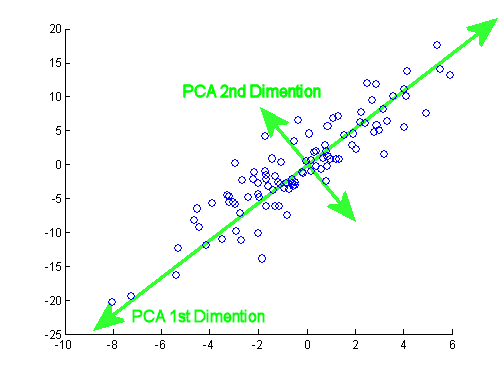
\includegraphics[width=0.5\linewidth]{\toplevelprefix/chapters/chapter1/figs/PCA.png}
    \caption{一个具有两个主成分的分布。}
    \label{fig:PCA}
\end{figure}
问题是从 $\x$ 的许多样本中找到子空间基 $\boldsymbol{U}$。估计子空间 $\boldsymbol{U}$ 的一个典型方法是最小化噪声的方差,也称为最小均方误差(MMSE):
\begin{equation}
    \min_{\boldsymbol{U}} \mathbb{E}\big[\|\boldsymbol{\epsilon}\|_2^2\big] = \mathbb{E}\big[\|\x - \boldsymbol{U} \z\|_2^2\big].
\end{equation}
请注意,这本质上是一个去噪任务:一旦正确找到了基 $\boldsymbol{U}$,我们就可以通过将带噪样本 $\x$ 投影到由 $\boldsymbol{U}$ 张成的低维子空间上来对其进行去噪:
\begin{equation}
\x \rightarrow \hat \x = \boldsymbol{U}\boldsymbol{U}^\top \x. 
\end{equation}
如果噪声很小,并且我们学习到了正确的低维子空间 $\boldsymbol{U}$,我们应该期望 $\x \approx \hat \x$。也就是说,PCA是自编码的一个特例:
\begin{equation}
    \x   \xrightarrow{\hspace{2mm} \boldsymbol{U}^\top\hspace{2mm}} \z  \xrightarrow{\hspace{2mm} \boldsymbol{U} \hspace{2mm}} \hat \x.
       \label{eqn:auto-encoding-PCA}
\end{equation}
只是在这里,由于数据结构简单,编码器 $\mathcal{E}$ 和解码器 $\mathcal{D}$ 都变成了简单的线性算子(投影和提升)。

这是统计学中的一个经典问题,称为主成分分析(PCA)。它最早由皮尔逊在1901年研究\cite{Pearson1901},后来由霍特林在1933年独立研究\cite{Hotelling1933}。这个主题在经典著作\cite{Jolliffe1986,JolliffeI2002}中有系统的总结。
此外,可以明确假设数据 $\x$ 根据一个单一的低维高斯分布:
\begin{equation}
    \x \sim \mathcal{N}(\boldsymbol{0}, \boldsymbol{U}\boldsymbol{U}^\top + \sigma \I), \quad \boldsymbol{U} \in \mathbb{R}^{D\times d},
\end{equation}
这等价于假设上述PCA模型\eqref{eqn:PCA-model}中的 $\z$ 是一个标准正态分布。
这被称为概率PCA\cite{TippingM1999}。

在本书中,我们将在第\ref{ch:classic}章中从学习低维分布的角度重新审视PCA。我们的目标是使用这个简单而理想化的模型来传达一些学习低维分布紧凑表示的最基本思想,包括通过去噪和自编码实现一致表示的重要概念。

\paragraph{独立成分分析。}
独立成分分析(ICA)最初由\cite{Ans-1985}提出,作为{\em 学习良好表示}的经典模型。事实上,它最初是作为我们记忆的一个简单数学模型提出的。ICA模型采用了与上述PCA模型\eqref{eqn:PCA-model}极其相似的形式,假设观测到的随机变量 $\x$ 是多个独立成分 $z_i$ 的线性叠加:
\begin{equation}
    \x = \boldsymbol{u}_1 z_1 + \boldsymbol{u}_2 z_2 + \cdots + \boldsymbol{u}_d z_d  + \boldsymbol{\epsilon} =  \boldsymbol{U} \z + \boldsymbol{\epsilon}.
    \label{eqn:ICA-model}
\end{equation}
然而,这里的成分 $z_i$ 被假定为独立的{\em 非高斯}变量。例如,一个流行的选择是
\begin{equation}
    z_i = \sigma_i \cdot w_i, \quad \sigma_i \sim B(1,p),
    \label{eqn:ICA-modes}
\end{equation}
其中 $\sigma_i$ 是一个伯努利随机变量,而 $w_i$ 可以是一个常数值或另一个随机变量,比如高斯变量。\footnote{即使 $w$ 是高斯变量,$\sigma w$ 也不再是高斯变量!} ICA问题试图从观测到的 $\x$ 样本中辨识出 $\boldsymbol{U}$ 和 $\z$。图\ref{fig:ICA-PCA}说明了ICA和PCA之间的区别。

\begin{figure}
    \centering
    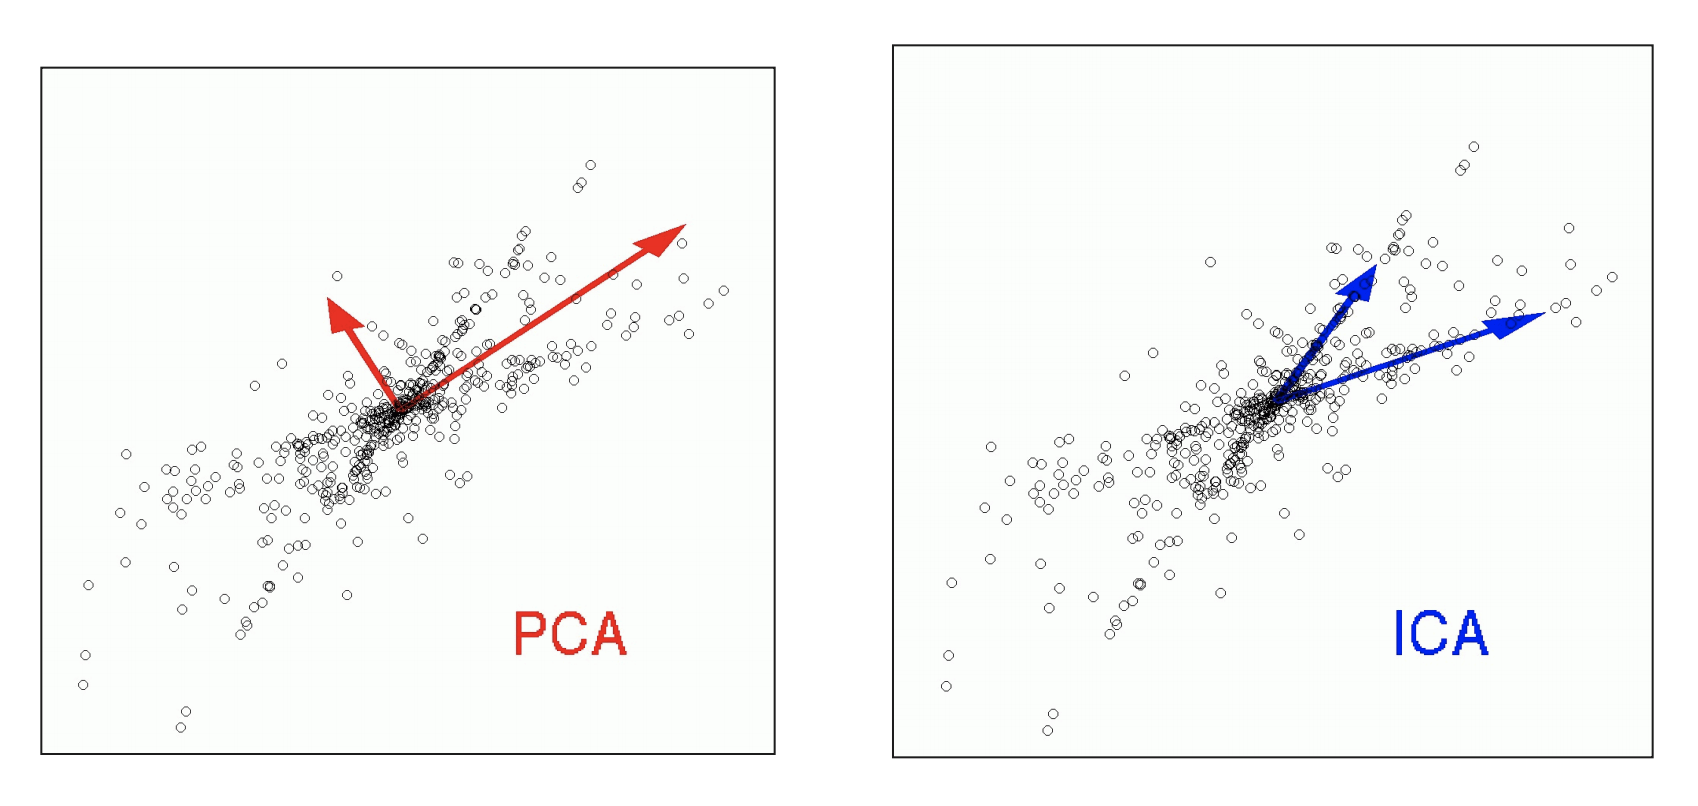
\includegraphics[width=0.7\linewidth]{\toplevelprefix/chapters/chapter1/figs/PCA_ICA.png}
    \caption{PCA(左)与ICA(右)的对比。}
    \label{fig:ICA-PCA}
\end{figure}

尽管一旦学习到 $\boldsymbol{U}$ 和 $\z$,从 $\z$ 到 $\x$ 的(解码)映射看起来是线性的且容易,但从 $\x$ 到 $\z$ 的(编码)映射可能很复杂,并且可能无法用简单的线性映射来表示。因此,ICA通常给出一个形式如下的自编码:
\begin{equation}
    \x   \xrightarrow{\hspace{2mm} \mathcal{E}\hspace{2mm}} \z  \xrightarrow{\hspace{2mm} \boldsymbol{U} \hspace{2mm}} \hat \x.
       \label{eqn:auto-encoding-ICA}
\end{equation}
因此,与PCA不同,ICA的分析和求解要困难一些。在1990年代,像Erkki Oja和Aapo Hyv\"{a}rinen\cite{hyvarinen-1997,Hyvrinen-2000}这样的人对ICA做出了重要的理论和算法贡献。在第\ref{ch:classic}章中,我们将研究并给出一个ICA的解决方案,从中编码映射 $\mathcal{E}$ 将变得清晰。



\paragraph{稀疏结构与压缩感知。}
可以看出,如果\eqref{eqn:ICA-modes}中的 $p$ 非常小,那么任何一个成分非零的概率都很小。在这种情况下,我们说 $\x$ 是稀疏生成的,它集中在一组维度为 $k = p \cdot d$ 的线性子空间上。因此,在某种程度上,我们可以将上述ICA模型扩展到一个更一般的低维结构族,即稀疏模型。

一个 $k$-稀疏模型被定义为由所有{\em $k$-稀疏向量}组成的集合:
\begin{equation}
    \mathcal{Z} = \{\z \in \mathbb{R}^n \mid \|\z\|_0 \le k\},
\end{equation}
其中 $\| \cdot \|_0$ 是 $\ell^0$-范数,它计算向量 $\z$ 中非零条目的数量。也就是说,$\mathcal{Z}$ 是所有与坐标轴对齐的 $k$ 维子空间的并集,如图\ref{fig:mixture-models}左侧所示。经典信号处理和统计学中的一个重要问题是如何从其线性观测中恢复一个稀疏向量 $\z$:
\begin{equation}
    \x = \boldsymbol{A} \z + \boldsymbol{\epsilon}, \quad \boldsymbol{A} \in \mathbb{R}^{m\times n}
    \label{eqn:sparse-model}
\end{equation}
其中 $\boldsymbol{A}$ 是给定的,但通常 $m < n$,$\boldsymbol{\epsilon}$ 是某个小噪声。这个看似无害的问题在计算上是NP难的,甚至难以近似(详见\cite{Wright-Ma-2022}一书)。

因此,尽管有着可以追溯到18世纪的非常丰富和悠久的研究历史\cite{Boscovichca1750},但并没有可证明有效解决这类问题的算法,尽管在1960年代到1990年代之间提出了许多启发式算法。有些在实践中相当有效,但没有任何严格的论证。一个重大的突破出现在2000年代初,当时包括David Donoho、Emmanuel Candès和Terence Tao在内的几位著名数学家\cite{donoho2005neighborly,Candes2005,CandesE2005-IT}建立了一个严格的理论框架,使我们能够精确地描述在什么条件下稀疏恢复问题可以被有效且高效地解决,例如通过凸$\ell^1$最小化:
\begin{equation}
    \min \|\z\|_1 \quad \mbox{subject to} \quad \| \x - \boldsymbol{A}\z\|_2 \le \epsilon,
\end{equation}
其中 $\|\cdot \|_1$ 是促进稀疏性的向量$\ell^1$范数,$\epsilon$ 是某个小常数。这个问题的任何解都实质上给出了一个稀疏编码映射:
\begin{equation}
    \x   \xrightarrow{\hspace{2mm} \mathcal{E} \hspace{2mm}}  \z.
       \label{eqn:decoding-sparse}
\end{equation}
我们将在第\ref{ch:classic}章中简要介绍这样一种算法,也就是映射,它将揭示稀疏编码和深度学习之间有趣的根本联系。\footnote{尽管稀疏编码算法和深度网络之间的相似性早在2010年就被注意到了\cite{gregor2010learning}。}

事实证明,$\ell^1$最小化成功的条件出人意料地普遍。成功恢复所需的最小测量次数 $m$ 仅与数据的内在维度 $k$ 成正比。这现在被称为{\em 压缩感知}现象\cite{CandesE2006-ICM}。此外,这种现象并非稀疏结构所独有。它也适用于非常广泛的低维结构族,如低秩矩阵等。这些结果从根本上改变了我们对在高维空间中恢复低维结构的理解。高维数据分析的这种戏剧性命运逆转甚至被David Donoho誉为“{\em 维度的祝福}”\cite{DonohoD2000},与通常对高维问题的“维度诅咒”的悲观信念形成对比。这一连贯而完整的成果体系已在\cite{Wright-Ma-2022}一书中得到系统组织。

从计算的角度来看,这个新框架的重要性不容小觑。它从根本上改变了我们对一类以前被认为基本上是棘手的问题的看法。它使我们能够开发出极其高效的算法,这些算法能够优雅地随问题维度扩展,从而使稀疏恢复问题从:
\begin{equation}
    \mbox{\textbf{棘手的}} \;
   \Longrightarrow \; \mbox{\textbf{可行的}} \; \Longrightarrow \; 
   \mbox{\textbf{可扩展的}}
\end{equation}
转变。这些算法还附带有严格的理论保证,确保在给定的数据和计算要求下其正确性。这种方法的严谨和精确性几乎与实践深度神经网络的方法相反,后者在很大程度上是经验性的。然而,尽管它们在风格和标准上看似对立,我们现在知道这两种方法都有一个共同的目标:{\em 试图在高维空间中追求低维结构。}

\paragraph{字典学习。}
从概念上讲,一个比稀疏编码问题\eqref{eqn:sparse-model}更难的问题是,当观测矩阵 $\boldsymbol{A}$ 事先未知,我们需要从一组(可能带噪的)观测,比如 $\X = [\x_1, \x_2, \ldots, \x_n]$ 中学习 $\boldsymbol{A}$:
\begin{equation}
    \X = \boldsymbol{A} \Z + \boldsymbol{E}, \quad \boldsymbol{A} \in \mathbb{R}^{m\times n}.
    \label{eqn:dictionary-learning}
\end{equation}
这里我们只给定了 $\X$,而没有相应的 $\Z = [\z_1, \z_2, \ldots, \z_n]$ 或噪声项 $\boldsymbol{E}= [\boldsymbol{\epsilon}_1, \boldsymbol{\epsilon}_2, \ldots, \boldsymbol{\epsilon}_n]$,只知道 $\z_i$ 是稀疏的。这被称为{\em 字典学习}问题,可以看作是前面讨论的ICA问题\eqref{eqn:ICA-model}的推广。换句话说,给定数据 $\X$ 的分布是在线性变换 $\boldsymbol{A}$ 下的标准稀疏分布 $\Z$ 的像,我们希望学习 $\boldsymbol{A}$ 及其“逆”映射 $\mathcal{E}$,从而得到一个自编码器:
\begin{equation}
    \X   \xrightarrow{\hspace{2mm} \mathcal{E} \hspace{2mm}}  \Z \xrightarrow{\hspace{2mm} \boldsymbol{A} \hspace{2mm}} \X?
       \label{eqn:decoding-DL}
\end{equation}

可以看出,PCA、ICA和字典学习的共同点是,它们都假设数据的分布支撑在低维线性或混合线性结构周围。它们都要求从可能是带噪的分布样本中学习(全局或局部的)线性结构基。在第\ref{ch:classic}章中,我们将研究如何通过这些经典模型来辨识低维结构。特别是,我们将看到一个有趣而重要的事实:所有这些低维(分段)线性模型都可以通过同一种快速算法——即{\em 幂迭代}\cite{Zhai-2020}——被有效且高效地学习。尽管上述线性或混合线性模型对于大多数真实世界的数据来说有些过于简单或理想化,但理解这些模型是理解更一般低维分布的重要第一步。

\subsubsection{一般分布}\label{sec:denoising-intro}

真实世界数据(如图像、视频和音频)的分布过于复杂,无法用上述有些理想化的线性模型或高斯过程来建模。我们通常事先不知道它们是由哪个参数模型族生成的。\footnote{尽管历史上曾有许多尝试为这些数据开发解析模型,例如用于图像数据的随机场或随机过程\cite{Mumford-1999},正如我们在前一节中讨论的那样。} 在实践中,我们通常只有来自它们分布的许多样本——即经验分布。显然,在这种情况下,我们通常不能期望对它们的低维结构有任何闭式解,也不能对由此产生的去噪算子有任何闭式解。\footnote{与PCA、维纳滤波器和卡尔曼滤波器的情况不同。} 因此,我们需要为这些经验分布开发一个更通用的解决方案,不一定是闭式解,但至少是高效可计算的。如果我们正确地做到了这一点,那么对上述线性模型的解决方案应该成为它们的特例。

\paragraph{去噪。} 在1950年代,统计学家对从任意分布中抽取的数据进行去噪的问题产生了兴趣。设 $\x_o$ 是一个概率密度函数为 $p_o(\cdot)$ 的随机变量。如果我们观察到 $\x_o$ 的一个带噪版本:
\begin{equation}
    \x = \x_o + \sigma \vg, 
\end{equation}
其中 $\vg \sim \dNorm(\vzero, \vI)$ 是标准高斯噪声,$\sigma$ 是观测的噪声水平。设 $p(\cdot)$ 是 $\x$ 的概率密度函数,\footnote{即 $p(\x) = \int_{-\infty}^{\infty} \phi_{\sigma}(\x - \z)p_o(\z) \odif{\z}$,其中 $\phi_{\sigma}$ 是高斯分布 $\mathcal{N}(\boldsymbol{0}, \sigma^2 \boldsymbol{I})$ 的密度函数。} 令人惊讶的是,给定 $\x$ 的 $\x_o$ 的后验期望可以通过一个优雅的公式计算,即特威迪公式\cite{Robbins1956AnEB}:\footnote{赫伯特·罗宾斯将这个公式的功劳归于他们私人通信中的莫里斯·肯尼思·特威迪。}
\begin{equation}
    \hat \x_o = \mathbb{E}[\x_o\mid \x] = \x + \sigma^2 \nabla \log p(\x).
\end{equation}
从公式中可以看出,函数 $\nabla \log p(\x)$ 在这里对观测 $\x$ 进行去噪起着非常特殊的作用。噪声 $\vg$ 可以明确地估计为
\begin{equation}
    \hat{\vg} = \frac{\x - \hat \x_o}{\sigma} = -\sigma \nabla \log p(\x),
\end{equation}
为此,我们只需要知道 $\x$ 的分布 $p(\cdot)$,而不需要知道 $\x_o$ 的真实分布 $p_o(\cdot)$。这个结果的一个重要含义是,如果我们将高斯噪声添加到任何分布中,只要我们能以某种方式得到函数 $\nabla \log p(\x)$,去噪过程就可以很容易地完成。

因为这是一个如此重要和有用的结果,它在许多不同的背景和领域被重新发现和使用。例如,在特威迪公式\cite{Robbins1956AnEB}之后,几年后它被\cite{Miyasawa61}重新发现。在2000年代初,函数 $\nabla \log p(\x)$ 在学习一般分布的背景下再次被重新发现,并被Aapo Hyv\"{a}rinen命名为“得分函数”\cite{hyvarinen05a}。但它与(经验贝叶斯)去噪的联系很快被\cite{Vincent2011}认识到。
对其他测量分布(高斯噪声之外)的推广已由Eero Simoncelli的研究组\cite{Raphan10}做出,并后来应用于图像去噪\cite{Kadkhodaie21a,ho2020denoising}。

\begin{figure}
    \centering
    %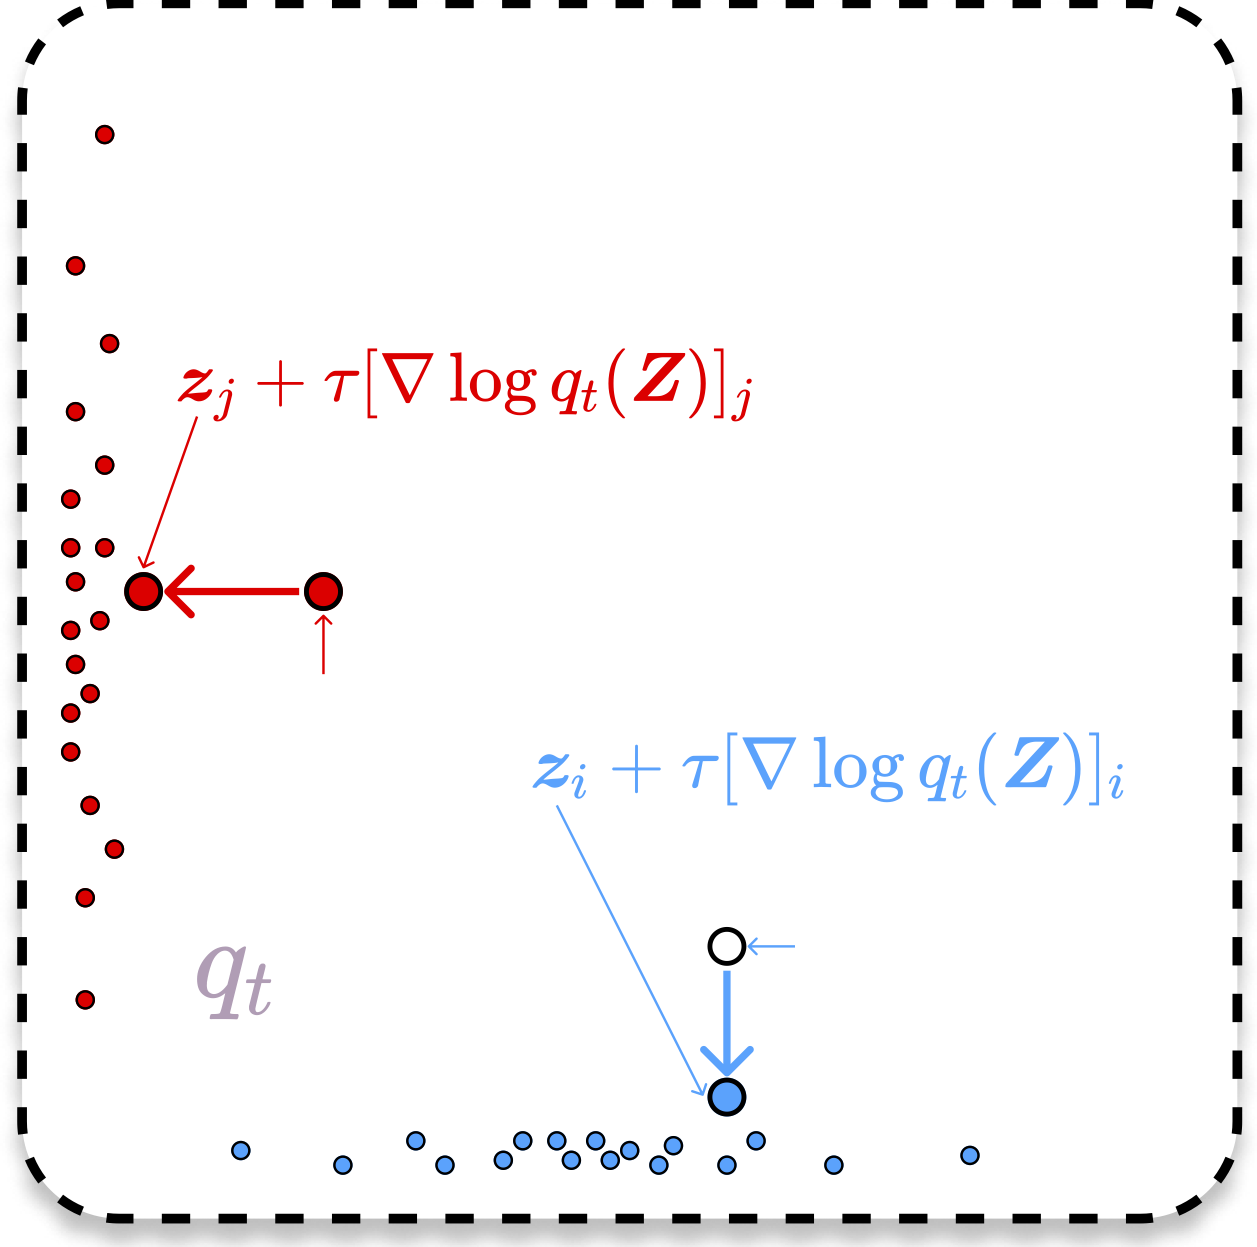
\includegraphics[width=0.45\linewidth]{\toplevelprefix/chapters/chapter1/figs/Score.png}
    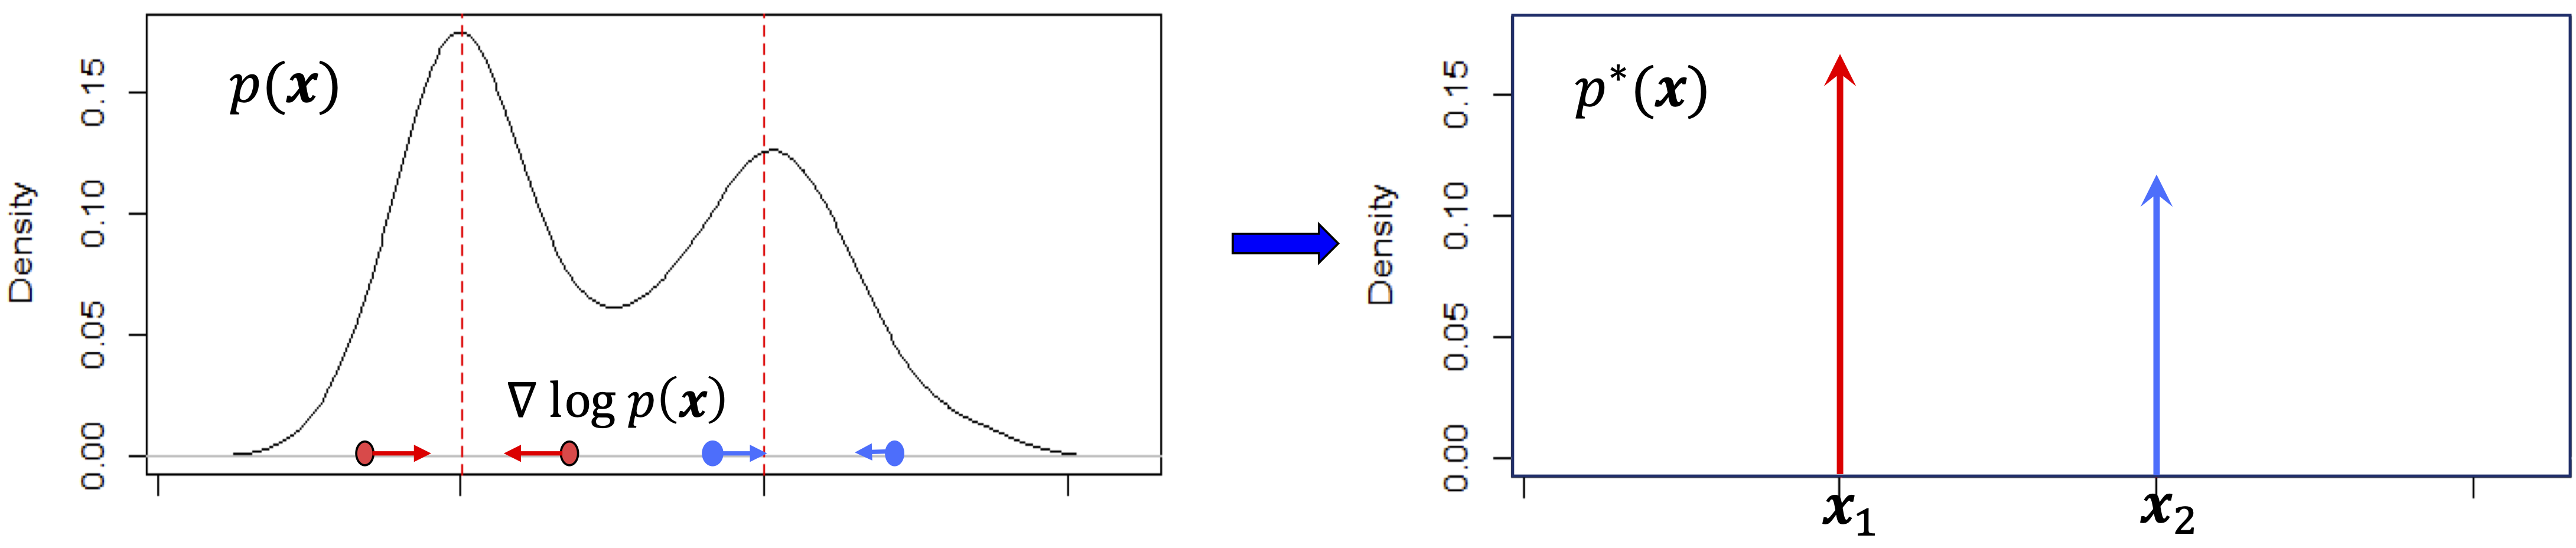
\includegraphics[width=1\linewidth]{\toplevelprefix/chapters/chapter1/figs/Density-compress.png}
    \caption{左侧是密度为 $p(\x)$ 的分布的得分函数 $\nabla \log p(\x)$ 的几何解释。由得分函数生成的操作将分布推向密度更高的区域。目标是,通过某种紧凑性度量(例如熵或编码长度),得到的分布更加“压缩”。最终,分布会收敛到一个具有较低维度支撑的分布,如右侧所示的 $p^*(\x)$。}
    \label{fig:score-function}
\end{figure}

\paragraph{熵最小化。} 事实上,这个函数有一个非常直观的信息论和几何解释。注意,在信息论中,$-\log p(\x)$ 通常对应于编码 $\x$ 所需的比特数\footnote{至少在离散变量的情况下是这样,我们将在第\ref{ch:compression}章中更详细地解释。}。梯度 $\nabla \log p(\x)$ 指向密度更高的方向,如图\ref{fig:score-function}左侧所示。如果 $\x$ 朝那个方向移动,编码它所需的比特数就会减少。因此,算子 $\nabla \log p(\x)$ 的总体效果是推动分布向密度更高的区域“收缩”。实际上,可以正式证明,分布的(微分)熵
\begin{equation}
H(\x) = - \int p(\boldsymbol{w}) \log p(\boldsymbol{w}) \odif{\boldsymbol{w}}    \end{equation} 
在这种操作下确实会减少(见第\ref{ch:compression}章和附录\ref{app:diffusion-denoising})。因此,如果我们用一个最优的码本对其进行编码,得到的分布的总体编码长度/率会降低,因此更加“压缩”。直观地,可以想象,如果我们无限地重复这样的去噪过程,分布最终会收缩到一个其质量集中在较低维度支撑上的分布。例如,图\ref{fig:score-function}左侧所示的分布 $p(\x)$,在得分函数 $\nabla \log p(\x)$ 的作用下,最终将收敛到右侧的分布 $p^*(\x)$\footnote{严格来说,$p^*(\x)$ 是一个其密度为广义函数的分布:$p^*(\x) = p^*(\x_1)\delta(\x-\x_1) + p^*(\x_2) \delta(\x-\x_2)$,其中 $p^*(\x_1) + p^*(\x_2) = 1$。}:
\begin{equation}
H(\x) = - \int p(\boldsymbol{w}) \log p(\boldsymbol{w}) \odif{\boldsymbol{w}}  \quad \xrightarrow{\hspace{1mm} \mbox{递减} \hspace{1mm}} \quad H^*(\x) = - \int p^*(\boldsymbol{w}) \log p^*(\boldsymbol{w}) \odif{\boldsymbol{w}}.    
\end{equation}
严格来说,当分布收敛到 $p^*(\x)$ 时,其微分熵收敛到负无穷大。这是由于连续随机变量和离散随机变量的微分熵定义存在技术差异。我们将在第\ref{ch:compression}章中看到如何使用更统一的{\em 率失真}度量来解决这个技术难题。


我们将在本章后面和第\ref{ch:compression}章中讨论,这样一个看似简单的去噪和压缩概念如何导出一个非常统一和强大的方法,用于学习高维空间中的一般低维分布,包括自然图像的分布。

\subsection{经验方法}
在实践中,对于许多重要的真实世界数据,如图像、声音和文本,很难用理想化的线性或混合线性模型来建模。例如,在图像处理和计算机视觉领域,有着悠久而丰富的历史,试图用解析方法对自然图像的分布进行建模。菲尔兹奖得主戴维·芒福德(David Mumford)在1990年代花费了大量精力试图理解和建模自然图像的统计特性\cite{Mumford1996TheSD}。他和他的学生,包括朱松纯,从统计物理学中汲取灵感和技术,提出了许多用于自然图像分布的统计和随机模型\cite{Zhu-Entropy-1997,Zhu1997LearningGP,Zhu1997Prior,Huang-Mumford,Mumford-1999,Lee-Mumford}。然而,这些解析模型在生成与自然图像非常相似的样本方面收效有限。显然,对于像图像这样的真实世界数据,我们需要开发更强大和统一的方法来追求它们更一般的低维结构。

因此,历史上,许多经验模型被提出来建模重要的真实世界数据,包括图像和文本。这些模型通常从生物神经系统的特征中汲取灵感,因为动物或人类的大脑似乎能极其高效和有效地处理这些数据。

\subsubsection{经典人工神经网络}
\paragraph{人工神经元。}

\begin{figure}[t]
    \centering
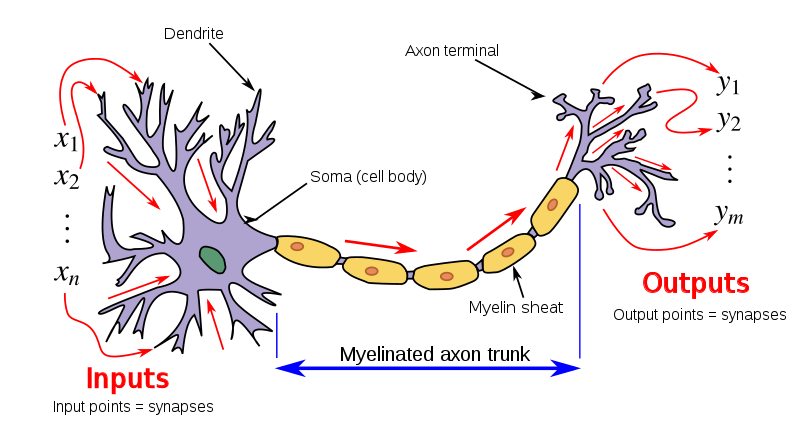
\includegraphics[width=0.55\linewidth]{\toplevelprefix/chapters/chapter1/figs/neuron.png} \hspace{3mm}   
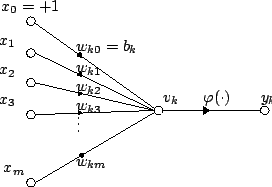
\includegraphics[width=0.40\linewidth]{\toplevelprefix/chapters/chapter1/figs/Artificial_neuron.png}
    \caption{第一个模仿神经元(左)如何处理信号的人工神经元(右)的数学模型。}
    \label{fig:neuron}
\end{figure}

受大脑神经系统的启发,第一个人工神经元\footnote{被称为线性阈值单元,或感知机。}的数学模型由沃伦·麦卡洛克\footnote{当时芝加哥大学的精神病学教授}和沃尔特·皮茨于1943年提出\cite{McCulloch-Pitts}。它描述了输入 $x_i$ 和输出 $o_j$ 之间的关系为:
\begin{equation}
    o_j = \varphi\Big( \sum_i w_{ji}x_i\Big),  
\end{equation}
其中 $\varphi(\cdot)$ 是某个非线性激活函数,通常用阈值函数建模。这个模型如图\ref{fig:neuron}所示。我们可以看到,这种形式已经具备了现代深度神经网络基本单元的主要特征。该模型源于对我们神经系统中单个神经元工作方式的观察。然而,人们并不确切知道这样一组神经元想要实现和执行什么功能。在更技术的层面上,他们也不确定应该使用什么样的非线性激活函数 $\varphi(\cdot)$。因此,历史上提出了许多变体。\footnote{阶跃函数、硬阈值或软阈值、整流线性单元(ReLU)、sigmoid等。
}

\begin{figure}[t]
\centering
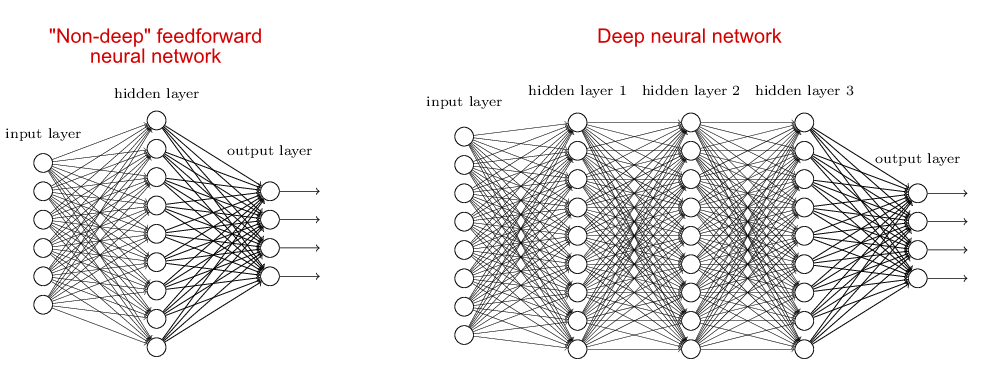
\includegraphics[width=0.85\linewidth]{\toplevelprefix/chapters/chapter1/figs/single-deep.png}
    \caption{一个单隐藏层网络(左)与一个深度网络(右)的对比。}
    \label{fig:single-deep}
\end{figure}
\paragraph{人工神经网络。}
在1950年代,弗兰克·罗森布拉特是第一个用这样的人工神经元{\em 网络}建造机器的人,如图\ref{fig:perceptron}所示。这台机器被称为Mark I感知机,它由一个输入层、一个输出层和一个包含512个人工神经元的单隐藏层组成,如图\ref{fig:perceptron}左侧所示,这与图\ref{fig:single-deep}左侧所示的类似。它被设计用来分类字母的光学图像。然而,单层网络的能力有限,只能学习线性可分的模式。在1969年马文·明斯基和西摩尔·派普特的著作《感知机:计算几何导论》\cite{Minsky-1969}中,证明了Mark I感知机的单层结构无法学习异或(XOR)函数。这一结果极大地削弱了人们对人工神经网络的兴趣,尽管后来证明多层网络能够学习异或函数\cite{Rumelhart1986}。事实上,一个(足够大的)多层网络,如图\ref{fig:single-deep}右侧所示,由这些简单的神经元组成,可以模拟任何有限状态机,甚至是通用图灵机。\footnote{不要混淆神经网络原则上能做什么与学习一个实现特定期望功能的神经网络是否可行或容易。} 尽管如此,随后,人工神经网络的研究在1970年代进入了它的第一个冬天。

\begin{figure}
    \centering
    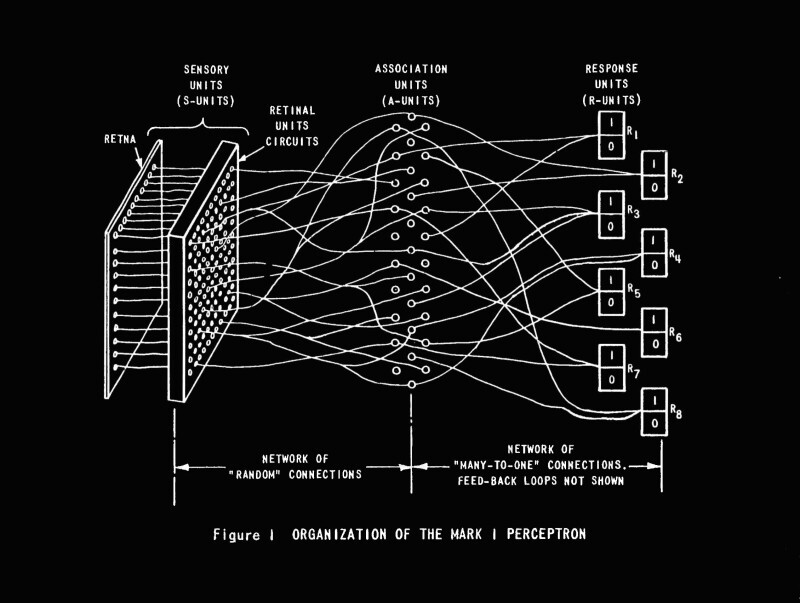
\includegraphics[width=0.45\linewidth]{\toplevelprefix/chapters/chapter1/figs/visu-large.jpg}
    \hspace{2mm} 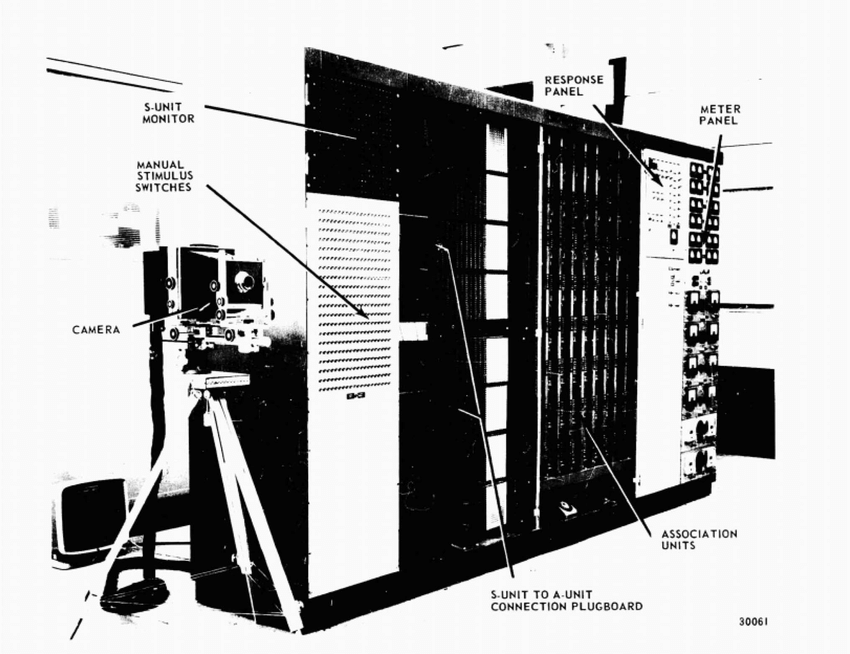
\includegraphics[width=0.45\linewidth]{\toplevelprefix/chapters/chapter1/figs/Original-Mark-I-perceptron-as-seen-in-its-operators-manual-20.ppm.png}
    \caption{弗兰克·罗森布拉特在1950年代末开发的Mark I感知机。}
    \label{fig:perceptron}
\end{figure}


\paragraph{卷积神经网络。}
1950年代和60年代对像Mark I感知机这样的人工神经网络的早期实验有些令人失望,这表明仅仅以多层感知机(MLP)的通用方式连接神经元可能是不够的。为了构建有效且高效的网络,我们需要理解网络中的神经元需要共同实现什么目的或功能,以便它们应该以某种特殊的方式组织和学习。再一次,机器智能的研究转向从动物神经系统的工作方式中汲取灵感。

众所周知,我们大脑的大部分都致力于处理视觉信息。在1950年代和1960年代,戴维·休伯尔和托尔斯滕·威泽尔系统地研究了猫的视觉皮层。他们发现视觉皮层包含不同类型的细胞(称为简单细胞和复杂细胞),这些细胞对不同方向和位置的视觉刺激敏感\cite{Hubel-Wiesel-1959}。休伯尔和威泽尔因其开创性的发现获得了1981年的诺贝尔生理学或医学奖。


在人工神经网络方面,休伯尔和威泽尔的工作启发了福岛邦彦,他在1980年设计了“神经认知机”(neocognitron)网络,该网络由模仿视觉皮层中生物神经元的人工神经元组成\cite{Fukushima1980NeocognitronAS}。这被认为是第一个{\em 卷积神经网络}(CNN),其架构如图\ref{fig:neocognitron}所示。与感知机不同,神经认知机有多个隐藏层,可以被看作是一个深度网络,如图\ref{fig:single-deep}右侧所示。

同样受到猫视觉皮层中神经元工作方式的启发,他也是第一个在1969年引入使用{\em 整流线性单元}(ReLU)的人\cite{Fukushima-1969}:
\begin{equation}
    \varphi(x) = \max\{0, x\} = \casework{x, & \text{if} \, x > 0, \\ 0, \quad & \text{if} \, x \leq 0,}
\end{equation}
作为激活函数 $\varphi(\cdot)$。但直到最近几年,ReLU才成为现代深度(卷积)神经网络中广泛使用的激活函数。一旦我们解释了深度网络试图实现的主要操作:压缩,我们将在本书中学习为什么这是一个好的选择。
%\yima{An image of a convolution neural network or the LeNet here...}

\begin{figure}
    \centering
    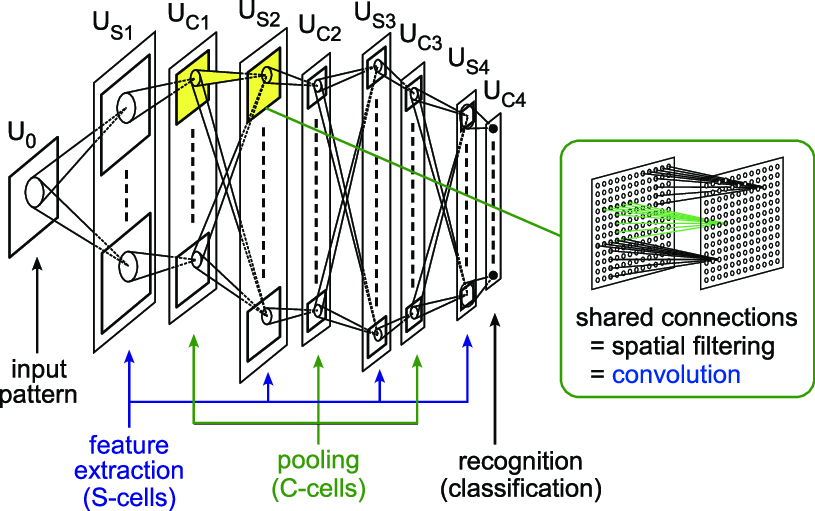
\includegraphics[width=0.6\linewidth]{\toplevelprefix/chapters/chapter1/figs/neocognitron.png}
    \caption{卷积神经网络的起源:福岛邦彦于1980年提出的神经认知机。请注意,卷积层和池化层的交错试图模仿在猫的视觉皮层中发现的简单细胞和复杂细胞的功能。}
    \label{fig:neocognitron}
\end{figure}

CNN类型的网络在1980年代继续发展,许多不同的变体被引入和研究。然而,尽管深度网络具有卓越的能力和受神经科学启发的改进架构,但为图像分类等实际任务训练这样的深度网络仍然极其困难。如何让一个网络工作依赖于许多无法解释的启发式方法和技巧,这确实限制了神经网络的吸引力和适用性。一个重大的突破出现在1989年左右,当时杨立昆(Yann LeCun)成功地使用{\em 反向传播}(BP)来学习一个用于识别手写数字的深度卷积神经网络\cite{LeCun-1989},后来被称为LeNet(见图\ref{fig:LeNet-5})。经过几年的不懈发展,他的坚持在1990年代末得到了回报:LeNet的性能最终变得足够好,可以用于实际应用\cite{LeCun-1998}:它被美国邮政局用于识别手写数字(用于邮政编码)。LeNet被认为是所有现代深度神经网络的“原型”,例如我们稍后将讨论的AlexNet和ResNet。由于这项工作,杨立昆被授予2018年图灵奖。\footnote{与另外两位深度网络的先驱,约书亚·本吉奥和杰弗里·辛顿共同获奖。}

\begin{figure}
    \centering
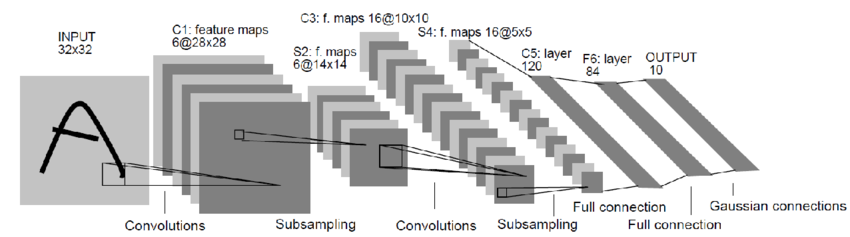
\includegraphics[width=0.95\linewidth]{\toplevelprefix/chapters/chapter1/figs/LeNet-5.png}
    \caption{杨立昆于1989年设计的LeNet-5卷积神经网络。}
    \label{fig:LeNet-5}
\end{figure}

\paragraph{反向传播。}
在历史上,深度神经网络的命运似乎与它们如何能够被轻松高效地训练紧密相连。反向传播(BP)就是为此而引入的。我们知道,一个多层感知机可以表示为一系列线性映射和非线性激活的复合:
\begin{equation}
h(\bm W_1, \ldots, \bm W_L) = f^L(\bm W_Lf^{L-1}(\bm W_{L-1} \cdots f^2(\bm W_2f^1(\bm W_1\x)))).
\end{equation}
为了基于梯度下降算法训练网络权重 $\{\bm W_l\}_{l=1}^L$ 以减少预测/分类误差,我们需要评估梯度 ${\partial h}/{\partial \bm W_l}$。众所周知,根据微积分中的{\em 链式法则},对于这类函数,梯度可以被高效地计算,后来被称为反向传播(BP)。详见附录\ref{app:optimization}。反向传播技术在1960年代和1970年代就已经被最优控制和动态规划等领域的人们所知晓和实践。例如,它出现在Paul Werbos博士1974年的博士论文中\cite{Werbos-1974, Werbos1994TheRO}。1986年,David Rumelhart等人首次将反向传播应用于训练多层感知机(MLP)网络\cite{Rumelhart1986}。从那时起,BP变得越来越流行,因为它提供了一个{\em 可扩展的}算法来学习大型深度神经网络。\footnote{因为它可以高效地在支持并行和分布式计算的计算平台上实现。} 它现在几乎是训练深度神经网络的主导技术。然而,人们相信自然界不是通过反向传播来学习的,因为这种机制对于自然界的物理实现来说仍然过于昂贵\footnote{正如我们之前讨论的,自然界几乎普遍通过闭环反馈来学习纠正错误。}。这显然为未来的改进留下了巨大的空间,我们将在后面更多地讨论。

然而,尽管1980年代取得了上述算法进展和有希望的实践,但训练深度神经网络对于1980年代和1990年代的计算系统来说仍然极其挑剔和昂贵。在1990年代末,支持向量机(SVM)\cite{SVM-1995}变得非常流行,因为它们被视为在分类等任务中优于神经网络的更好选择。\footnote{事实上,解决分类问题的类似思想可以追溯到Thomas Cover的博士论文工作,该工作被浓缩并发表在1964年的一篇论文中\cite{Cover-1964}。} 有两个主要原因:首先,SVM基于一个严格的统计学习框架,即Vapnik-Chervonenkis(VC)理论;其次,它导致了基于凸优化\cite{BoydVa04}的相当高效的算法。SVM的兴起在2000年代初给神经网络的研究带来了第二个冬天。

\paragraph{压缩自编码。}
在1980年代末和1990年代,人工神经网络已经被用来学习高维数据(如图像)的低维表示。已经证明,神经网络可以用来从数据中学习PCA\cite{Oja1982SimplifiedNM,Baldi89},而不是使用第\ref{sec:PCA-ICA}节中讨论的经典方法。在1980年代末,也有人认为,由于其模拟非线性变换的能力,神经网络被建议用于学习具有非线性分布的数据的低维表示。与线性PCA情况类似,可以尝试同时学习一个非线性降维编码器 $f$ 和一个解码器 $g$,每个都由一个深度神经网络建模\cite{Rumelhart1986,Kramer1991NonlinearPC}:
\begin{equation}
    \X   \xrightarrow{\hspace{2mm} f \hspace{2mm}} \Z  \xrightarrow{\hspace{2mm} g \hspace{2mm}} \hat \X.
       \label{eqn:auto-encoding-deep-networks}
\end{equation}
通过强制解码后的数据 $\hat \X$ 与原始数据 $\X$ 一致,例如通过最小化一个MMSE类型的重构误差\footnote{尽管MMSE类型的误差对于具有复杂非线性结构的图像数据来说已知是有问题的。正如我们很快将讨论的,生成方法(包括GAN)最近的许多工作都是为了找到原始数据 $\X$ 和再生数据 $\hat \X$ 之间更好的距离函数的替代品。}:
\begin{equation}
    \min_{f,g} \big\|\X - \hat \X\big\|_2^2 = \big\|\X - g(f( \X))\big\|_2^2,
\end{equation}
一个自编码器可以从数据 $\X$ 本身学习到。

但是我们如何保证这样的自编码确实捕捉到了 $\X$ 中真正的低维结构,而不是给出一个琐碎的冗余表示呢?例如,我们可以简单地选择 $f$ 和 $g$ 为恒等映射,使得 $\Z = \X$。因此,为了确保自编码是有价值的,人们希望得到的表示是压缩的,即通过某种可计算的复杂度度量来衡量。1993年,杰弗里·辛顿及其同事提出使用编码长度作为这样的度量,因此自编码的目标变成了找到最小化编码长度的表示\cite{Hinton-1993}。这项工作还建立了最小描述长度原则\cite{Rissanen-1978}和自由(亥姆霍兹)能最小化之间的根本联系。辛顿小组后来的工作\cite{Hinton504}凭经验表明,这样的自编码能够为真实世界的图像学习有意义的低维表示。Pierre Baldi在2011年对自编码器做了更全面的综述\cite{Baldi2011},就在深度网络变得流行之前。我们将在本章后面的第\ref{sec:unifying-approach}节中更多地讨论复杂度度量和自编码,并在第\ref{ch:consistent}章中以更统一的视角系统地研究压缩自编码。


\begin{figure}
    \centering
    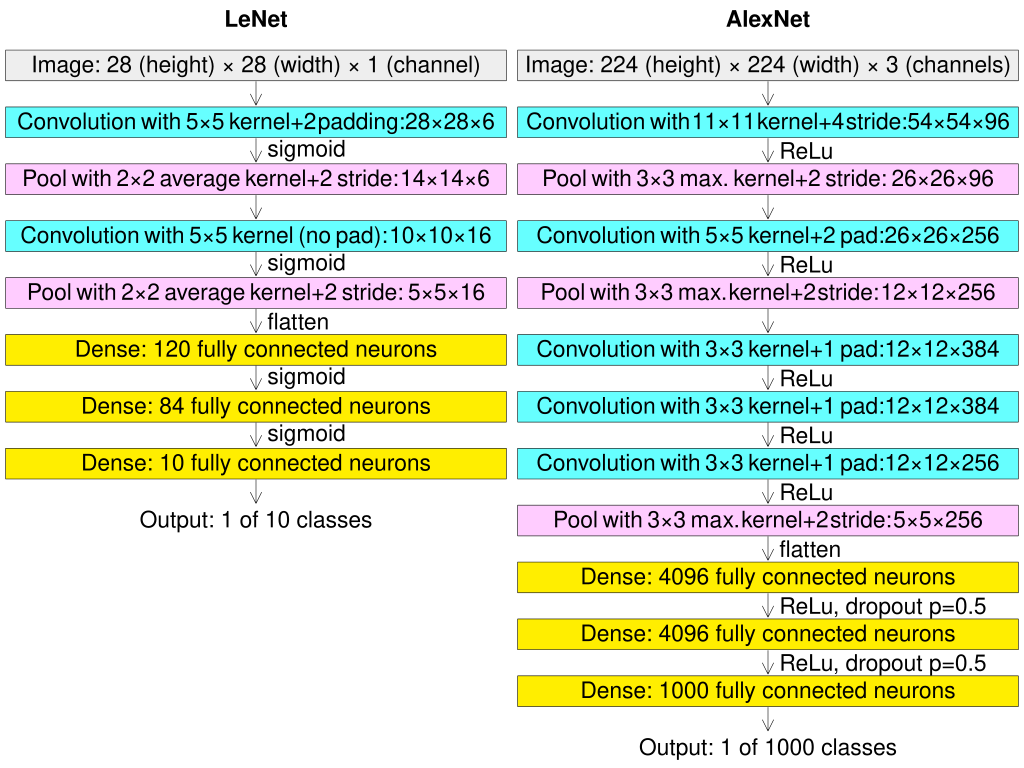
\includegraphics[width=0.8\linewidth]{\toplevelprefix/chapters/chapter1/figs/Comparison_image_neural_networks.svg.png}
    \caption{LeNet \cite{LeCun-1989} 与 AlexNet \cite{krizhevsky2012imagenet} 的架构对比。}
    \label{fig:LeNet-AlexNet}
\end{figure}


\subsubsection{现代深度神经网络}
从1980年代到2010年代的近30年里,对于机器学习和机器智能的研究,神经网络并未被主流认真对待。早期的(深度)神经网络,如LeNet,在识别数字等小规模分类问题上表现出有希望的性能。然而,网络的设计和实践相当经验化,当时可用的数据集很小,而BP算法对于当时的计算机来说是一个巨大的计算负担。这些因素导致了对神经网络兴趣的缺乏,进展停滞不前,只有少数研究人员在从事这项工作。

\paragraph{分类与识别。}
事实证明,只有当有足够的数据和计算能力时,深度神经网络的巨大潜力才能被释放出来。快进到2010年代,像ImageNet这样的大型数据集变得可用,GPU也变得足够强大,使得BP变得更加经济实惠,即使对于比LeNet大得多的网络也是如此。大约在2012年,一个名为AlexNet的深度卷积神经网络引起了人们的注意,因为它在ImageNet数据集上以显著的优势超越了现有的分类方法\cite{krizhevsky2012imagenet}。\footnote{事实上,在此之前,深度网络已经在语音识别任务上展示了最先进的性能。但在它们在图像分类上取得成功之前,并没有受到太多关注。} 图\ref{fig:LeNet-AlexNet}显示了AlexNet和LeNet之间的比较。AlexNet与LeNet有许多共同的特点,只是它更大,并采用了ReLU作为非线性激活函数,而不是LeNet中使用的Sigmoid函数。部分由于这项工作的影响,杰弗里·辛顿被授予2018年图灵奖。


这一早期的成功激励了机器智能社区,在接下来的几年里,探索网络设计的新变体和改进。特别是,人们凭经验发现,网络越大越深,在图像分类等任务中的性能就越好。许多深度网络架构被尝试、测试和推广。一些著名的包括VGG\cite{Simonyan15}、GoogLeNet\cite{Szegedy2014GoingDW}、ResNet\cite{He2016-lc},以及最近的Transformers\cite{vaswani2017attention}等。尽管在经验性能上取得了快速进展,但对于这些凭经验发现的架构,缺乏理论解释,包括它们之间是否存在任何关系。本书的一个目的是揭示所有这些网络可能服务的共同目标,以及为什么它们共享某些共同的特征,包括多层线性算子与非线性激活交错(见第\ref{ch:representation}章)。

\paragraph{强化学习。}
深度网络早期的成功主要是在监督学习环境下的分类任务,如语音识别和图像识别。深度网络后来被由Demis Hassabis领导的DeepMind团队采用,用于学习玩游戏的决策或控制策略。在这种情况下,深度网络被用来建模最优决策/控制策略或相关的最优价值函数,如图\ref{fig:Alpha-Go}所示。这些网络参数根据玩游戏时当前策略的成功或失败返回的奖励,逐步进行优化\footnote{比如说基于反向传播(BP)。}。这种学习方法通常被称为{\em 强化学习}\cite{Sutton-Barto},起源于1960年代末控制系统的实践\cite{Waltz1965AHA,Mendel1970ReinforcementlearningCA}。其更早的根源可以追溯到1950年代理查德·贝尔曼的{\em 动态规划}\cite{Bellman-DP}和马文·明斯基的{\em 试错学习}\cite{Minsky-1954}的更长久和丰富的历史。

从实现的角度来看,深度网络和强化学习的结合被证明是相当强大的:深度网络可以用来近似那些难以用解析方法建模的真实世界环境的控制策略和价值函数。这种实践最终导致了由DeepMind公司开发的AlphaGo系统,它在2016年击败了顶尖人类棋手李世石,然后在2017年击败了世界冠军柯洁,震惊了世界。\footnote{1996年,IBM的深蓝系统通过击败俄罗斯国际象棋特级大师加里·卡斯帕罗夫创造了历史。它主要使用传统的机器学习技术,如树搜索和剪枝,这些技术不那么可扩展,并且在20多年里没有被证明在像围棋这样更具挑战性的游戏中成功。}

AlphaGo的成功令计算界大为惊讶,他们普遍认为搜索的状态空间大得令人望而却步,不可能有任何高效的解决方案,无论是在计算上还是在样本大小上。对其成功的唯一合理解释是,围棋游戏的最优价值/策略函数中必定存在非常好的结构。它们的内在维度不是很高,并且可以被一个神经网络很好地近似,这个网络可以从不是多得令人望而却步的样本中学习。

\begin{figure}
    \centering
    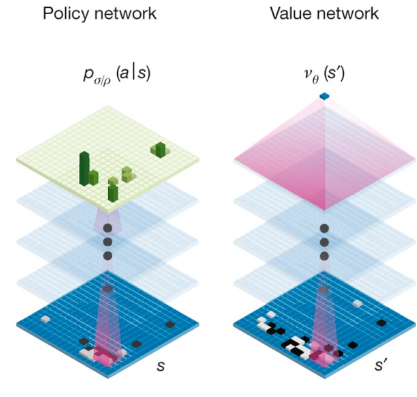
\includegraphics[width=0.5\linewidth]{\toplevelprefix/chapters/chapter1/figs/Policy-Value.png}
    \caption{AlphaGo:使用深度神经网络为围棋游戏建模最优策略或最优价值函数。}
    \label{fig:Alpha-Go}
\end{figure}

\paragraph{生成与预测。}
可以认为,2010年代深度网络的早期实践更侧重于从数据 $\X$ 中提取相关信息,并将其编码为特定任务的表示 $\Z$(例如,在分类任务中,$\Z$ 代表类别标签):
\begin{equation}
    \X   \xrightarrow{\hspace{2mm} f \hspace{2mm}} \Z.
       \label{eqn:encoding-deep-networks}
\end{equation}
在这种设置下,要学习的映射 $f$ 不需要保留关于 $\X$ 的大部分分布信息,而只需要特定任务所需的充分统计量。例如,$\X$ 中的一个样本 $\x$ 可能是一张苹果的图像,它被 $f$ 映射到其类别标签 $\z =$ “苹果”。2015年提出的{\em 信息瓶颈框架}\cite{Tishby-ITW2015}就是为了分析深度网络在这种背景下的作用。
 
然而,在许多现代情况下,例如所谓的“大基础模型”,人们通常需要解码 $\Z$ 以在一定精度上恢复相应的 $\X$:
\begin{equation}
    \Z   \xrightarrow{\hspace{2mm} g  \hspace{2mm}} \hat \X.
       \label{eqn:decoding-deep-networks}
\end{equation}
由于 $\X$ 通常代表从外部世界观察到的数据,一个好的解码器将允许我们模拟或预测世界上发生的事情。例如,在“文本到图像”或“文本到视频”任务中,$\z$ 通常代表描述所需图像 $\x$ 内容的文本。解码器应该能够生成一个与 $\x$ 内容相同的 $\hat \x$。例如,给定一个对象类别 $\z = $ “苹果”,解码器 $g$ 应该生成一张看起来像苹果的图像 $\hat \x$,尽管不一定与原始的 $\x$ 完全相同。



\paragraph{通过判别式方法进行生成。}
为了使生成的图像 $\hat \X$ 与真实的自然图像 $\X$ 相似,我们需要能够评估和最小化某个距离:
\begin{equation}
    \min d(\X, \hat \X).
\end{equation}
事实证明,对于高维空间中但具有低内在维度的分布,大多数理论上合理的距离都极其难以(如果不是不可能的话)计算和优化。\footnote{即使给定了 $\X$ 的参数化分布族,情况也是如此。对于具有低维支撑的分布,距离通常会变得病态或不明确。更糟糕的是,所选择的族可能无法很好地近似感兴趣的真实分布。}

2007年,朱松纯的前学生屠卓文,可能对早期用解析方法建模和生成自然图像的尝试感到失望(如前所述),决定尝试一种截然不同的方法。在CVPR 2007发表的一篇论文中\cite{Tu-2007},他首次提出可以通过判别式方法学习图像的生成模型。这个想法很简单:如果评估距离 $d(\X, \hat \X)$ 很困难,可以尝试学习一个判别器 $d$ 来区分 $\hat \X$ 和 $\X$:
\begin{equation}
    \Z   \xrightarrow{\hspace{2mm} g  \hspace{2mm}} \hat \X, \X \xrightarrow{\hspace{2mm} d  \hspace{2mm}} \boldsymbol{0}, \boldsymbol{1},
       \label{eqn:gan-networks}
\end{equation}
其中 $\boldsymbol{0}, \boldsymbol{1}$ 表示图像是生成的还是真实的。
直观地说,我们越难区分 $\hat \X$ 和 $\X$,它们可能就越接近。

屠的工作\cite{Tu-2007}首次展示了通过判别式方法学习生成模型的可行性。然而,该工作采用了传统的方法来生成图像和分类分布(如boosting),这些方法速度慢且难以实现。2012年后,深度神经网络在图像分类方面变得非常流行。2014年,Ian Goodfellow及其同事再次提出用判别式方法生成自然图像\cite{Goodfellow-2014}。他们建议使用深度神经网络来建模生成器 $g$ 和判别器 $d$。此外,他们提出通过一个极小极大博弈来学习生成器 $g$ 和判别器 $d$:
\begin{equation}
    \min_g \max_d \ell(\X, \hat \X),
\end{equation}
其中 $\ell(\cdot)$ 是与分类相关的某个自然损失函数。换句话说,判别器 $d$ 试图最大化其区分 $\X$ 和 $\hat \X$ 的成功率,而生成器 $g$ 则试图做相反的事情。因此,这种方法被命名为{\em 生成对抗网络}(GANs)。研究表明,在大型数据集上训练后,GANs确实可以生成照片般逼真的图像。部分由于这项工作的影响,约书亚·本吉奥被授予2018年图灵奖。

判别式方法似乎是绕过分布学习中一个基本困难的相当聪明的方式。然而,严格来说,这种方法并没有完全解决这个基本困难。\cite{Goodfellow-2014}的研究表明,在适当选择损失函数的情况下,极小极大公式在数学上等价于最小化 $\X$ 和 $\hat \X$ 之间的{\em Jensen-Shannon距离}(见\cite{Cover-Thomas})。对于高维空间中的两个低维分布来说,这是一个已知难题。因此,在实践中,GANs通常依赖于许多启发式方法和工程技巧,并常常遭受诸如{\em 模式坍塌}等不稳定性问题。\footnote{尽管如此,这样的极小极大公式为距离提供了一个实用的近似。它简化了实现,并避免了直接计算距离时的一些陷阱。} 总的来说,关于如何改进GANs的实践,一直缺乏理论指导。

\paragraph{通过去噪和扩散进行生成。}
2015年,在GAN被引入并变得流行后不久,Surya Ganguli和他的学生意识到并提出,一个由深度网络建模的迭代去噪过程可以用来学习一个通用分布,例如自然图像的分布\cite{Sohl-Dickstein2015}。他们的方法受到特殊高斯和二项过程性质的启发,这些性质由William Feller早在1949年研究过\cite{Feller1949OnTT}。\footnote{又是在神奇的1940年代!}
\begin{figure}[t]
    \centering
    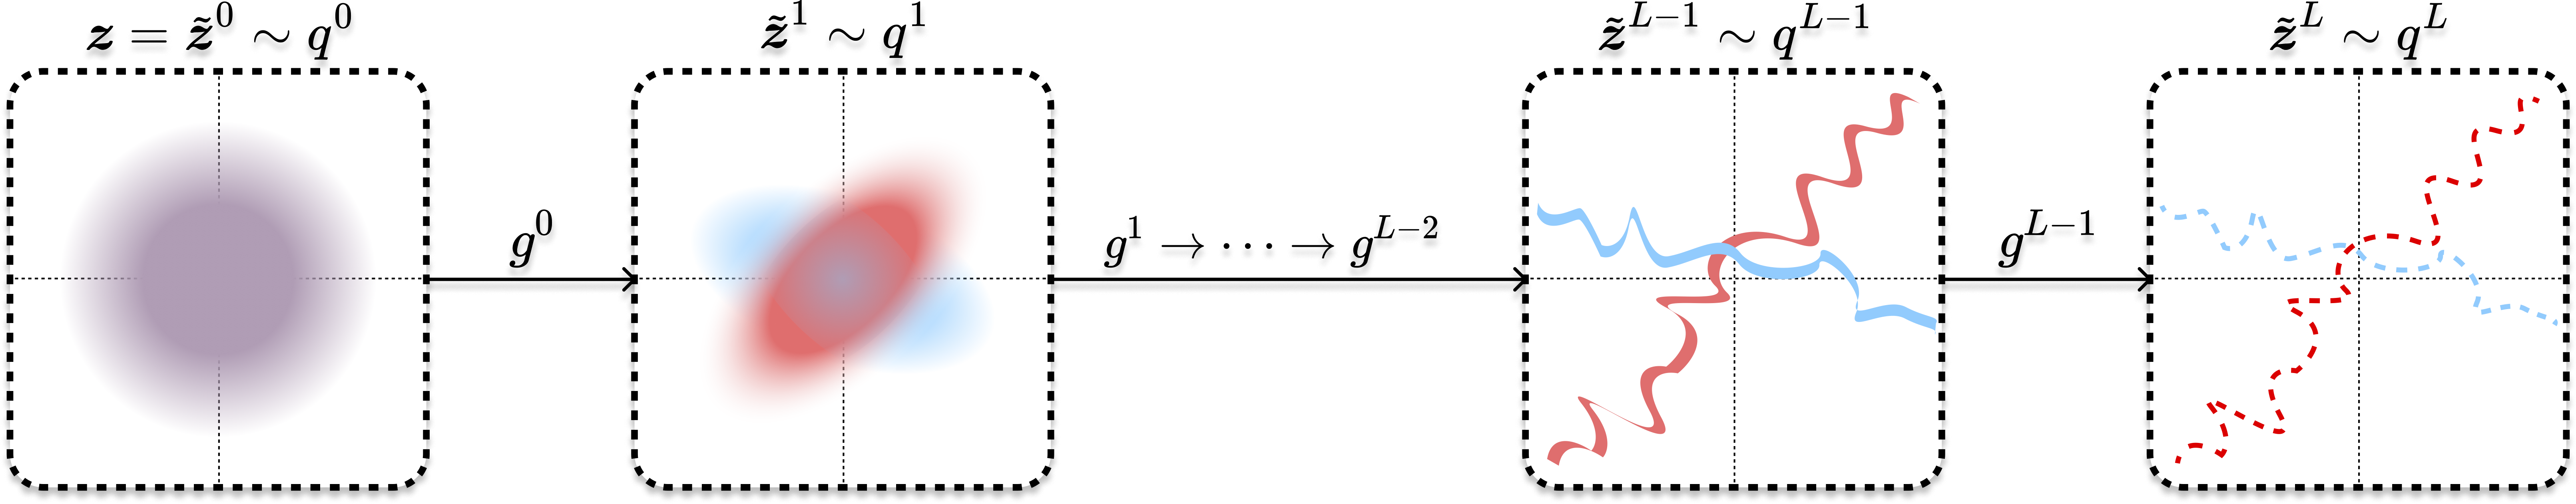
\includegraphics[width=\linewidth]{\toplevelprefix/chapters/chapter1/figs/diffusion_pipeline.png}
    \caption{一个迭代去噪和压缩过程的图示,从一个高斯分布 $q^0 = \mathcal{N}(\boldsymbol{0}, \boldsymbol{I})$ 开始,收敛到一个任意的低维数据分布 $q^L = p(\x)$。}
    \label{fig:diffusion}
\end{figure}

不久,基于得分函数\cite{hyvarinen05a}(在第\ref{sec:denoising-intro}节中简要介绍过)的去噪算子被证明更具通用性,并统一了去噪和扩散过程及算法\cite{song2019,song2020score,ho2020denoising}。图\ref{fig:diffusion}展示了将一个通用高斯分布 $q^0 = \mathcal{N}(\boldsymbol{0}, \boldsymbol{I})$ 转换为一个(任意的)经验分布 $p(\x)$ 的过程,通过执行一系列迭代去噪(或压缩)操作:
\begin{equation}
        \z^0 \sim  \mathcal{N}(\boldsymbol{0}, \boldsymbol{I})\xrightarrow{\hspace{2mm} g^0  \hspace{2mm}} \z^1 \xrightarrow{\hspace{2mm} g^1 \hspace{2mm}} \cdots \xrightarrow{\hspace{2mm} g^{L-1}  \hspace{2mm}} \z^L \sim p(\x).
\end{equation}
到目前为止,去噪(和扩散)已经取代了GANs,成为学习图像和视频分布的主流方法,催生了像Midjourney和Stability.ai这样的流行商业图像生成引擎。
在第\ref{ch:compression}章中,我们将系统地介绍和研究用于学习一般低维分布的去噪和扩散方法。



\section{一种统一的方法}\label{sec:unifying-approach}
到目前为止,我们已经简要介绍了机器智能的主要目标和历史,以及与之相关的许多重要思想和方法。近年来,在深度神经网络取得经验性成功之后,人们付出了巨大的努力来发展理论框架,以帮助我们理解所有凭经验设计的深度神经网络,无论是某些看似必要的组件(例如,dropout、归一化、注意力等)还是它们的整体行为(例如,双下降、神经坍塌等)。

部分受此启发,本书旨在实现几个重要且具有挑战性的目标:
\begin{itemize}
    \item 发展一个理论框架,使我们能够对深度神经网络进行严格的数学解释。
    \item 确保学习到的数据分布的正确性以及与学习到的表示的一致性。
    \item 证明该框架可以产生高性能的架构,并能指导实践中的进一步改进。
\end{itemize}
在过去几年中,越来越多的证据表明,通过利用前面简要讨论过的经典解析低维模型的理论和解决方案(在第\ref{ch:classic}章中更深入地探讨),并整合来自几个相关领域(即信息/编码论、控制/博弈论和优化)的基本思想,这些目标确实可以实现。本书旨在对这种新方法进行系统的介绍。

\subsection{学习简约表示}
\label{sec:computational-approach-compression}
任何学习任务成为可能的必要条件是,感兴趣的序列必须是{\em 可计算的},至少在艾伦·图灵\cite{Turing-1936}的意义上是这样。也就是说,一个序列可以通过一个程序在典型的计算机上计算出来。\footnote{确实存在定义明确但不可计算的序列。} 除了可计算之外,我们要求计算是{\em 可行的}。\footnote{我们不需要考虑预测那些计算复杂度是棘手的,比如在序列的长度或维度上呈指数增长的事物。} 也就是说,学习和计算序列的计算成本(空间和时间)不应呈指数增长。此外,正如我们在自然界(以及在现代机器智能实践中)所看到的,对于大多数实际任务,智能系统需要从高维空间中的海量数据(如视觉、声音和触觉)中学习可预测的东西。因此,对于智能,我们不需要考虑所有可计算和可行的序列或结构。我们应该只关注那些其学习和计算算法具有{\em 可扩展性}实现的可预测序列和结构:
\begin{equation}
\mbox{\textbf{可计算的}} \;
   \Longrightarrow \; \mbox{\textbf{可行的}} \; \Longrightarrow \; 
   \mbox{\textbf{可扩展的}}。
\end{equation}

这是因为智能生物用来学习有用信息的任何算法都必须是{\em 可扩展的}。更具体地说,算法的计算复杂度最好能优雅地扩展,通常是线性的甚至亚线性的,与数据的大小和维度相关。在技术层面上,这要求算法所依赖的学习操作只能利用可以从数据中高效计算的谕示信息。更具体地说,当维度高、规模大时,唯一能负担得起的谕示是数据的一阶几何信息\footnote{例如用线性子空间局部逼近非线性结构,并计算目标函数的梯度。}或二阶统计信息\footnote{例如数据或其特征的协方差或相关性。}。
本书的主要目标是发展一个理论和计算框架,在这个框架内,我们可以系统地开发高效且有效的解决方案或算法,利用这种可扩展的谕示和操作来从采样数据中{\em 学习}低维结构,并随后学习预测函数。


\paragraph{通过压缩追求低维性。}
从我们在第\ref{sec:predictability}节中给出的序列例子可以看出,有些序列容易建模和计算,而另一些则更困难。显然,一个序列的计算成本取决于预测函数 $f$ 的复杂程度。回归的阶数 $d$ 越高,计算成本就越高。$f$ 可以是一个简单的线性函数,也可以是一个任意难以指定和计算的非线性函数。

有理由相信,如果一个序列,无论我们选择何种度量,更难以指定和计算,那么从其采样片段中学习它也会更困难。然而,对于任何给定的可预测序列,实际上有许多,通常是无限多种方式来指定它。例如,对于一个简单的序列 $x_{n+1} = a x_{n}$,我们也可以用 $x_{n+1} = a x_n + b x_{n-1} - b x_{n-1}$ 来定义同一个序列。
因此,如果我们能为任何给定的可计算序列发展一个客观而严格的“复杂度”概念,那将非常有用。

俄罗斯数学家安德雷·柯尔莫哥洛夫是第一个为任何可计算序列给出复杂度定义的人之一。\footnote{许多人对这个序列复杂度的概念做出了贡献,最著名的包括雷·所罗门诺夫和格雷戈里·蔡廷。这三位都被认为独立地发展和研究了算法信息论,雷·所罗门诺夫在1960年,安德雷·柯尔莫哥洛夫在1965年\cite{Kolmogorov1998OnTO},格雷戈里·蔡廷在1966年左右\cite{Chaitin-1966}。} 他建议,在所有能计算同一个序列的程序中,我们可以使用最短程序的长度作为其复杂度的度量。这个想法与著名的“奥卡姆剃刀”简约原则非常一致:{\em 在所有能解释同一观察的理论中,总是选择最简单的那个。} 更准确地说,让 $p$ 代表一个可以在通用计算机 $\mathcal{U}$ 上生成序列 $S$ 的计算程序。序列 $S$ 的柯尔莫哥洛夫复杂度定义为:
\begin{equation}
    K(S) = \min_{p\,:\, \mathcal{U}(p) = S} L(p). 
\end{equation}
因此,一个序列的复杂度是通过我们能多么“简约地”指定或计算它来衡量的。这个复杂度的定义,或简约性,具有重要的概念意义,并有许多有趣的性质。历史上,它启发了计算理论中许多深刻的研究,特别是在算法信息论领域。

最短程序的长度可以被看作是所考虑序列的最终压缩,为我们通过学习序列的正确生成机制获得了多少信息提供了一个定量的度量。然而,尽管其理论重要性,柯尔莫哥洛夫复杂度通常不是一个可计算的函数\cite{Cover-Thomas}(甚至难以准确近似)。因此,这个复杂度度量在实践中用处不大。它既不能提前告诉我们学习一个给定序列有多困难,也不能告诉我们我们学得有多好。





%Measure of parsimony or compactness: Many (largely equivalent) ways to measure compactness of data: Kolmogorov complexity (not computable), dimension and volume of (the support of) the data distribution, minimum description length, rate distortion etc. 

\paragraph{可计算的简约性度量。}
因此,出于实践目的,我们需要一个对由同一预测函数生成的序列的高效可计算的复杂度度量。\footnote{请注意,在实践中,我们通常关心的是学习预测函数 $f$,而不是由 $f$ 生成的任何特定序列。} 请注意,柯尔莫哥洛夫复杂度不可计算的部分原因在于其定义是非构造性的。

因此,为了引入一个可计算的复杂度度量,我们可以采取一种更具构造性的方法,正如克劳德·香农通过信息论框架\cite{Shannon-1948,Cover-Thomas}所倡导的那样。\footnote{该框架在过去80多年里成功地指导了通信行业的工程实践。} 实质上,通过假设序列 $S$ 是从一个概率分布 $p(S)$ 中抽取的,该分布的所谓{\em 熵}:\footnote{这里我们考虑微分熵,因为我们假设序列由连续变量组成。如果它由离散变量组成,我们可以考虑熵:$H(S) = - \sum_{i}p(s_i) \log p(s_i)$。}
\begin{equation}
    h(S) \doteq -\int p(s) \log p(s) \odif{s}
    \label{eqn:entropy-definition}
\end{equation}
为其复杂度提供了一个自然的度量。这个度量还有一个自然的解释,即编码这样一个序列所需的平均比特数,我们将在第\ref{ch:compression}章中看到。

为了说明这个观点的主要思想,让我们取大量的长序列片段:
\begin{equation}
    \{S_1, S_2, \ldots, S_i, \ldots, S_N\} \subset \mathbb{R}^D,
\end{equation}
这些片段由一个预测函数 $f$ 生成。请注意,不失一般性,这里我们假设所有序列的长度都相同,为 $D$。因此,每个序列都可以看作是 $\mathbb{R}^D$ 中的一个向量。其次,我们可以引入一个编码方案(带有一个码本),记为 $\mathcal E$,它将每个片段 $S_i$ 转换为一个唯一的二进制比特流 $\mathcal{E}(S_i)$。最简单的编码方案是用 $\epsilon$-球填充所有片段所张成的空间,如图\ref{fig:coding-schemes}所示。然后我们给所有的球编号。每个序列被编码为其最近的球的(二进制)编号。因此,每个片段可以从其对应的比特流中恢复\footnote{精度达到 $\epsilon$,因为这样的编码方案是有损的。}。
\begin{figure}
    \centering
    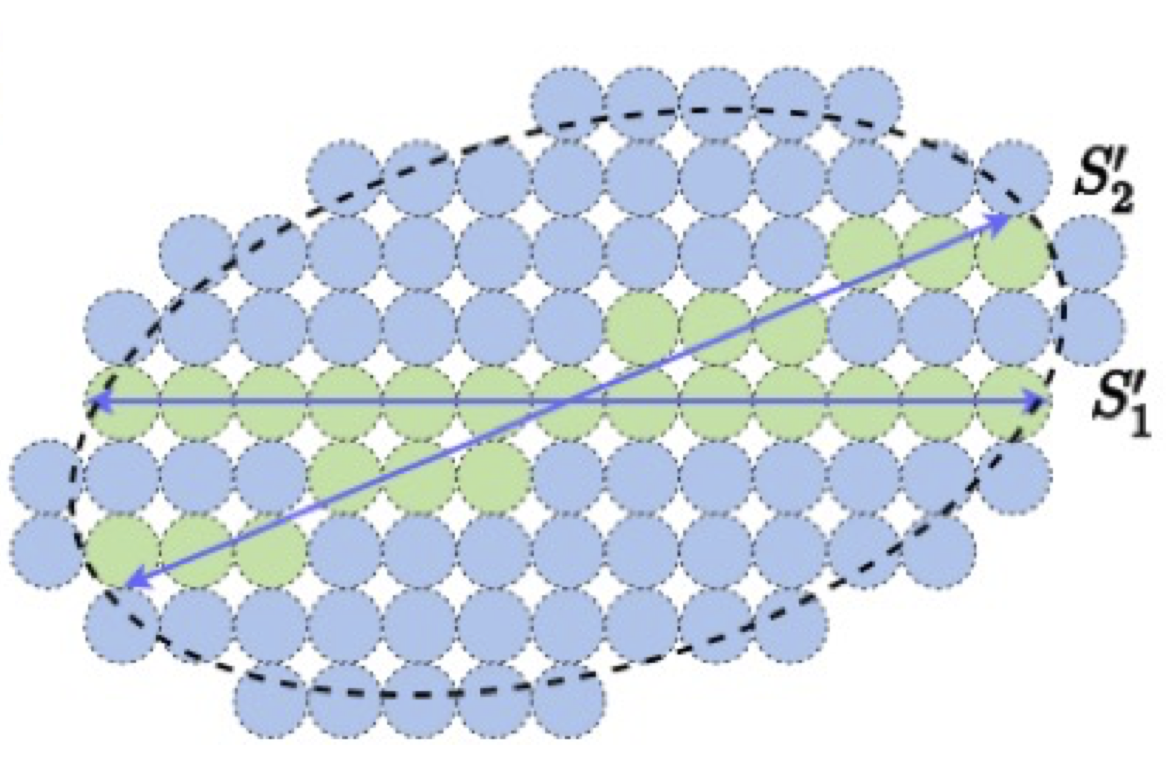
\includegraphics[width=0.5\linewidth]{\toplevelprefix/chapters/chapter1/figs/Coding-schemes.png}
    \caption{两种编码方案的比较。想象数据的真实分布在两条带箭头的线周围。可以用由所有蓝色球组成的码本来编码来自这两条线的样本;也可以用只由绿色球组成的码本来编码样本。显然,在相同精度下,第二种编码方案将导致低得多的编码长度/率。}
    \label{fig:coding-schemes}
\end{figure}


那么,预测函数 $f$ 的复杂度可以评估为所有序列的平均编码长度,即编码率:\footnote{我们可以通过将 $R(f\mid \mathcal{E})$ 取为所有长度为 $D$ 的片段的期望编码长度来使其更精确。}
\begin{equation}
   R(f \mid \mathcal E) = \mathbb{E}[L(\mathcal{E}(S))] \approx \frac{1}{N}\sum_{i=1}^N L(\mathcal{E}(S_i)). 
   \label{eqn:coding-rate}
\end{equation}
显然,如果使用不同的编码方案(或码本),编码率度量将会改变。在实践中,我们越了解片段分布所在的低维结构,我们就能设计出越高效的码本,如图\ref{fig:coding-schemes}所示的例子。敏锐的读者可能已经认识到,概念上,图\ref{fig:diffusion}中所示的去噪过程与从使用蓝色球的编码方案到使用绿色球的编码方案的过程非常相似。


给定两个用于片段的编码方案 $\mathcal{E}_1$ 和 $\mathcal{E}_2$,如果编码率的差异为正:
\begin{equation}
   R(f \mid \mathcal E_1) -  R(f \mid \mathcal E_2) > 0, 
\end{equation}
我们可以说编码方案 $\mathcal{E}_2$ 更好。这个差异可以被看作是 $\mathcal{E}_2$ 相对于 $\mathcal{E}_1$ 对数据分布拥有多少额外信息的度量。在很大程度上,学习 $f$ 的目标等同于找到最小化编码率的最有效编码方案:
\begin{equation}
   \min_{\mathcal{E}} R(f \mid \mathcal E). 
\end{equation}
正如我们将在第\ref{ch:compression}章中看到的,可达到的最小率与熵 $H(S)$ \eqref{eqn:entropy-definition}的概念密切相关。


\begin{remark}\label{rem:computable-complexity}
    {用显式编码方案来度量数据复杂度的观点,激发了几种旨在修正柯尔莫哥洛夫复杂度以获得更好可计算性的学习目标\cite{WallaceC1999},包括后来在1968年提出的最小消息长度(MML)\cite{WallaceC1968}和1978年提出的最小描述长度(MDL)\cite{Rissanen-1978,HansenM2001}。这些目标通常除了计算感兴趣的数据 $S$ 的编码长度外,还计算编码方案 $\mathcal{E}$ 本身(包括其码本)的编码长度:$L(\mathcal E(S)) + L(\mathcal E)$。然而,如果目标是学习一个有限大小的码本并将其应用于大量的序列,那么码本的摊销成本可以忽略不计,因为当 $N$ 变得很大时,$$\frac{1}{N}\Big( L(\mathcal{E}) + \sum_{i=1}^N L(\mathcal{E}(S_i))\Big) \approx \frac{1}{N}\sum_{i=1}^N L(\mathcal{E}(S_i))$$。}
\end{remark}

再次,我们可以将得到的最优编码方案看作是实现了对观测数据的最佳压缩的方案。总的来说,与柯尔莫哥洛夫复杂度相比,任何编码方案给出的编码长度总是更大的:
\begin{equation}
    K(S) < L( \mathcal E(S)).
\end{equation} 
因此,最小化编码率/长度本质上是最小化原本不可计算的柯尔莫哥洛夫复杂度的一个上界。

\subsection{学习信息丰富的表示}
%\paragraph{Structured representations via information gain.}
请注意,如果目标仅仅是为了压缩而压缩给定的数据,那么理论上,接近柯尔莫哥洛夫复杂度的最优编码将变得几乎是随机或无结构的\cite{Chaitin-1966}。\footnote{因为任何有结构的编码都可以被进一步压缩。} 然而,我们学习预测函数 $f$ 的真正目的是为了在未来的预测中能够轻松地重复使用它。因此,虽然压缩使我们能够辨识数据中的低维分布,但我们希望以一种结构化和有组织的方式对分布进行编码,以便得到的表示信息丰富且使用高效。\footnote{例如,在不同条件下对分布进行采样。} 图\ref{fig:expansion}用一个例子直观地解释了为什么需要这样的变换。

\begin{figure}
    \centering
    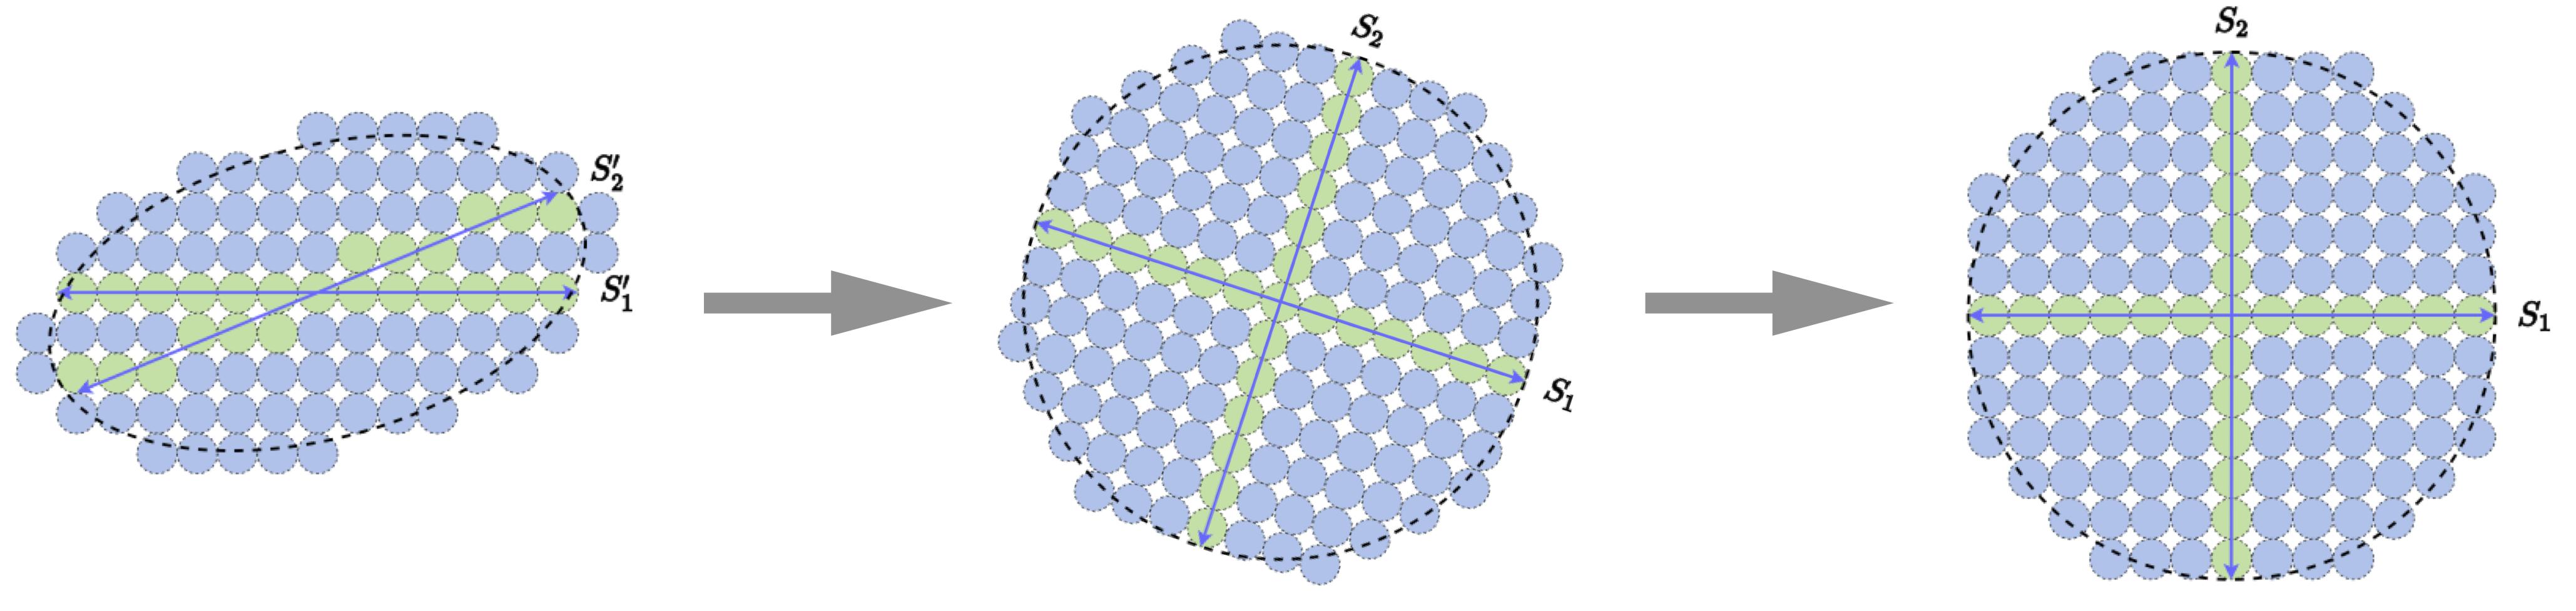
\includegraphics[width=0.98\linewidth]{\toplevelprefix/chapters/chapter1/figs/coding-transform.png}
    \caption{将辨识出的低维数据分布转换为一个信息更丰富、结构更清晰的表示。}
    \label{fig:expansion}
\end{figure}
正如我们将在第\ref{ch:compression}章中展示的,最终表示中这些期望的结构可以通过选择一个基于所选编码方案编码率的自然{\em 信息增益}度量来精确地促进。正如我们在本书中将看到的,这种显式和构造性的编码方法为学习真实世界数据的低维结构的良好表示提供了一个强大的计算框架,因为在许多具有实际重要性的情况下,编码长度函数可以被高效地计算或准确地近似。在一些良性情况下,我们甚至可以得到闭式公式,例如子空间和高斯分布(见第\ref{ch:compression}章)。

此外,这样的计算框架导出了一个有原则的方法,自然地揭示了深度网络在这个学习过程中所扮演的角色。正如我们将在第\ref{ch:representation}章中系统地推导的,深度网络的各层试图以增量的方式执行优化感兴趣目标函数的操作。从这个角度来看,深度网络的作用可以被精确地解释为模拟某个迭代优化算法,比如梯度下降,来优化信息增益的目标。由此产生的深度架构的各层可以被赋予精确的统计和几何解释,即执行增量的压缩编码和解码操作。结果是,推导出的深度网络变成了数学上完全可解释的透明“白盒”。



% \textbf{Notes:} Convert predictability to low-dimensionality: A universal mathematical property of such data is that their distribution always has very low intrinsic dimensions, hence highly compressible, in the usually high-dimensional space they are embedded. 

% %Additional correlations that promote low-dimensionality, such as many physical laws described by partial differential equations, e.g. Maxwell equations for electric magnetic fields and Navier Stokes equations for fluid dynamics. 

% Measure of compactness: Many (largely equivalent) ways to measure compactness of data: Kolmogorov complexity (not computable), dimension and volume of (the support of) the data distribution, minimum description length, rate distortion etc. 

% Hence, one effective way to learn low-dimensional structures inherited from predictability is through certain operations of ``compression'' (which we will make precise later) that aim to minimize such measures. 





\subsection{学习一致的表示}

%\subsection{Ensuring Consistency}
\label{sec:consistency}
为了总结我们到目前为止的讨论,让我们将数据表示为:
\begin{equation}
    \boldsymbol{X} = \{S_1, S_2, \ldots, S_i, \ldots, S_N\} \subset \mathbb{R}^D,
\end{equation}
并让 $\boldsymbol{Z} = \mathcal{E}(\X)$ 是通过某个编码器 $\mathcal{E}$ 对 $\X$ 进行编码的结果:
\begin{equation}
    \X  \xrightarrow{\hspace{2mm} \mathcal{E}\hspace{2mm}} \Z.
    \label{eqn:open-loop}
\end{equation}
在机器学习的背景下,$\Z$ 通常被称为“特征”或“潜在表示”。请注意,在不知道 $\X$ 的底层分布的情况下,我们不知道哪个编码器 $\mathcal{E}$ 能够保留关于 $\X$ 分布的最有用信息。在实践中,人们通常从尝试某种能很好地服务于特定任务的紧凑编码方案开始。特别是,他们会尝试学习一个能够优化学习表示的某种(经验)简约性度量的编码器:
\begin{equation}
    \min \rho(\Z). 
\end{equation}

\begin{example}
例如,图像分类就是这样一个例子:我们将同一类别的所有图像分配给一个单一的编码,不同类别的图像分配给不同的编码,比如“独热”向量:
\begin{equation}
  \x \mapsto \z \in \{  [1, 0, 0, \ldots , 0, 0], \;  [0, 1, 0 \ldots, 0, 0], \; \ldots, \;  [0,0,0, \ldots, 0, 1].\}
  \label{eqn:class-labels}
\end{equation}
现在,一个分类器 $f(\cdot)$ 可以被建模为一个函数,它预测给定 $\x$ 属于 $K$ 个类别中每一个的概率:$\hat{\z} = f(\x) \in \mathbb{R}^K$。那么,一个分类器的“好坏”可以通过所谓的{\em 交叉熵}来衡量:\footnote{交叉熵可以被看作是 $\z$ 的真实分布和预测 $\hat\z$ 的分布之间的距离度量。它也可以被看作是如果我们使用 $\hat \z$ 的最优码本来编码 $\z$ 时,$\z$ 的期望编码长度。当 $\z$ 和 $\hat \z$ 具有相同分布时,交叉熵达到最小值。}
\begin{equation}
    L(\hat{\z}, \z) = \sum_{k=1}^K - z_k \log \hat{z}_k,
\end{equation}
其中 $z_k$ 表示向量 $\z$ 的第 $k$ 个条目。正如深度网络的早期实践所表明的\cite{krizhevsky2012imagenet},如果给定了足够的数据,这样的编码方案通常可以由一个深度网络来表示,并通过优化交叉熵以端到端的方式学习。
\end{example}

交叉熵损失 $L(\hat \z, \z)$ 可以被看作是与一类特别适合分类的编码方案相关的简约性度量 $\rho(\z)$ 的一个特例。然而,这样的编码显然是{\em 非常有损的}。学习到的 $\z$ 除了其类别类型外,不包含关于 $\x$ 的任何其他信息。例如,通过将一张图像分配给(代表)类别标签“苹果”的编码,我们仅从标签本身无法知道原始图像中是哪种特定类型的苹果。

当然,另一个极端是要求编码方案是{\em 无损的}。也就是说,$\x$ 和其编码 $\z$ 之间存在一一映射。然而,正如我们将在第\ref{ch:compression}章中看到的,无损编码(或压缩)是不切实际的,除非 $\x$ 是离散的。对于一个连续随机变量,我们只能考虑有损编码方案,以便数据的编码长度可以是有限的。也就是说,我们只将数据编码到某个预定的精度。正如我们将在第\ref{ch:compression}章中进一步阐述的,有损编码不仅仅是一个实际的选择,它在从有限的分布样本中学习底层连续分布方面起着根本性的作用。

对于许多学习目的,我们希望特征 $\z$ 虽然是{\em 有损的},但能比仅仅是其类别类型保留更多关于 $\x$ 的信息。在本书中,我们将介绍一个更通用的基于编码长度/率的简约性度量,它与一类更通用的编码方案——用子空间或高斯混合体进行编码——相关联。这个族有能力以一定的精度紧密近似任意的真实世界分布。正如我们将在第\ref{ch:compression}章和第\ref{ch:representation}章中看到的,这样的度量不仅能保留关于 $\X$ 分布的大部分信息,而且还能为学习到的表示 $\Z$ 促进某些期望的良好几何和统计结构。


\paragraph{用于一致性的双向自编码。}
在更广泛的学习背景下,一个压缩编码方案 $\mathcal{E}$ 的主要目标是辨识数据 $\X$ 中的低维结构,以便它们可以被用来预测原始数据空间中的事物。这要求学习到的编码方案 $\mathcal{E}$ 允许一个高效的解码方案,记为 $\mathcal D$。它将 $\Z$(通常称为潜在表示)映射回数据空间:
\begin{equation}
    \X   \xrightarrow{\hspace{2mm} \mathcal{E}\hspace{2mm}} \Z  \xrightarrow{\hspace{2mm} \mathcal{D} \hspace{2mm}} \hat \X.
       \label{eqn:auto-encoding}
\end{equation}
一般来说,我们称这样的编码和解码对 $(\mathcal{E}, \mathcal{D})$ 为一个{\em 自编码}。图\ref{fig:autoencoder}
展示了这样一个自编码器的过程。
\begin{figure}
    \centering
    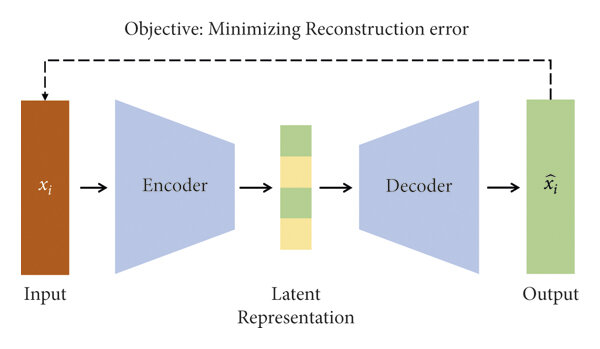
\includegraphics[width=0.7\linewidth]{\toplevelprefix/chapters/chapter1/figs/Autoencoder.jpg}
    \caption{一个自编码器架构的图示。}
    \label{fig:autoencoder}
\end{figure}


通常,我们希望解码在某种程度上是编码的近似“逆”,使得从 $\Z$ 解码出的数据(分布)$\hat \X$ 与原始数据(分布)$\X$ 在某种程度上相似。\footnote{我们稍后将更精确地说明我们所说的相似是什么意思。} 如果是这样,我们将能够从 $\Z$ 中恢复或预测原始数据空间中发生的事情。在这种情况下,我们说对 $(\mathcal{E}, \mathcal{D})$ 给出了一个{\em 一致的}自编码。对于大多数实际目的,我们不仅需要这样的解码存在,而且还需要它可以被高效地实现和物理地实现。例如,如果 $\x$ 是一个实值变量,为了任何解码方案能在有限状态机上实现,就需要进行量化,我们将在第\ref{ch:compression}章中更多地解释。因此,总的来说,我们应该期望可实现的编码和解码方案必然是有损的。一个核心问题是如何学习一个紧凑的(有损的)表示 $\Z$,以便它可以被用来很好地预测 $\X$。

总的来说,正如我们将看到的,编码器和解码器都可以由深度网络建模和实现,并通过解决以下形式的优化问题来学习:
\begin{equation}
   \min \, d( \X, \hat \X) + \rho(\Z), 
   \label{eqn:auto-encoding-objective}
\end{equation}
其中 $d(\cdot, \cdot)$ 是一个促进 $\X$ 和 $\hat \X$ 之间相似性的距离函数\footnote{可以是样本级的相似,也可以是分布级的相似,取决于距离函数 $d$ 的选择。},$\rho(\Z)$ 是某个促进 $\Z$ 的简约性和信息丰富性的度量。经典的主成分分析(PCA)\cite{JolliffeI2002}是一致自编码的一个典型例子,我们将在第\ref{ch:classic}章中详细研究它,作为更一般低维结构的前奏。在第\ref{ch:autoencoding}章中,我们将研究如何为一般的(比如非线性的)低维分布学习一致的自编码。


\subsection{学习自洽的表示}
请注意,在上述自编码目标中,需要评估解码后的数据 $\hat \X$ 与原始数据 $\X$ 的接近或一致程度。这通常需要一些外部监督或关于使用何种相似性度量的知识。计算 $\hat \X$ 和 $\X$ 之间的相似性可能非常昂贵,如果不是完全不可能或棘手的话。\footnote{比如说,人们想要最小化两者之间的某种分布距离。} 请注意,在自然界中,动物能够完全靠自己学习,而无需将其估计的 $\hat \X$ 与数据空间中的真实 $\X$ 进行比较。它们通常甚至没有这个选项。

那么,一个系统如何在没有外部监督或比较的情况下自主学习呢?它们如何知道 $\hat \X$ 与 $\X$ 是一致的,即使没有直接比较它们?这就引出了“闭环”的思想。事实证明,在我们将在第\ref{ch:closed-loop}章中精确化的温和条件下,为了确保 $\X$ 和 $\hat \X$ 是一致的,只需要将 $\hat \X$ 编码为 $\hat \Z$,并检查 $\Z$ 和 $\hat \Z$ 是否一致。我们将这种一致性概念称为{\em 自洽性},它可以通过以下图示来说明:
\begin{equation}
    \X   \xrightarrow{\hspace{2mm} \mathcal{E}\hspace{2mm}} \Z  \xrightarrow{\hspace{2mm} \mathcal{D} \hspace{2mm}} \hat \X \xrightarrow{\hspace{2mm} \mathcal{E}\hspace{2mm}} \hat \Z,
    \label{eqn:closed-loop}
\end{equation}
我们将这个过程称为{\em 闭环转录},\footnote{灵感来自于DNA和RNA或其他蛋白质之间的转录过程。} 如图\ref{fig:closed-loop}所示。

\begin{figure}[t]
\centering{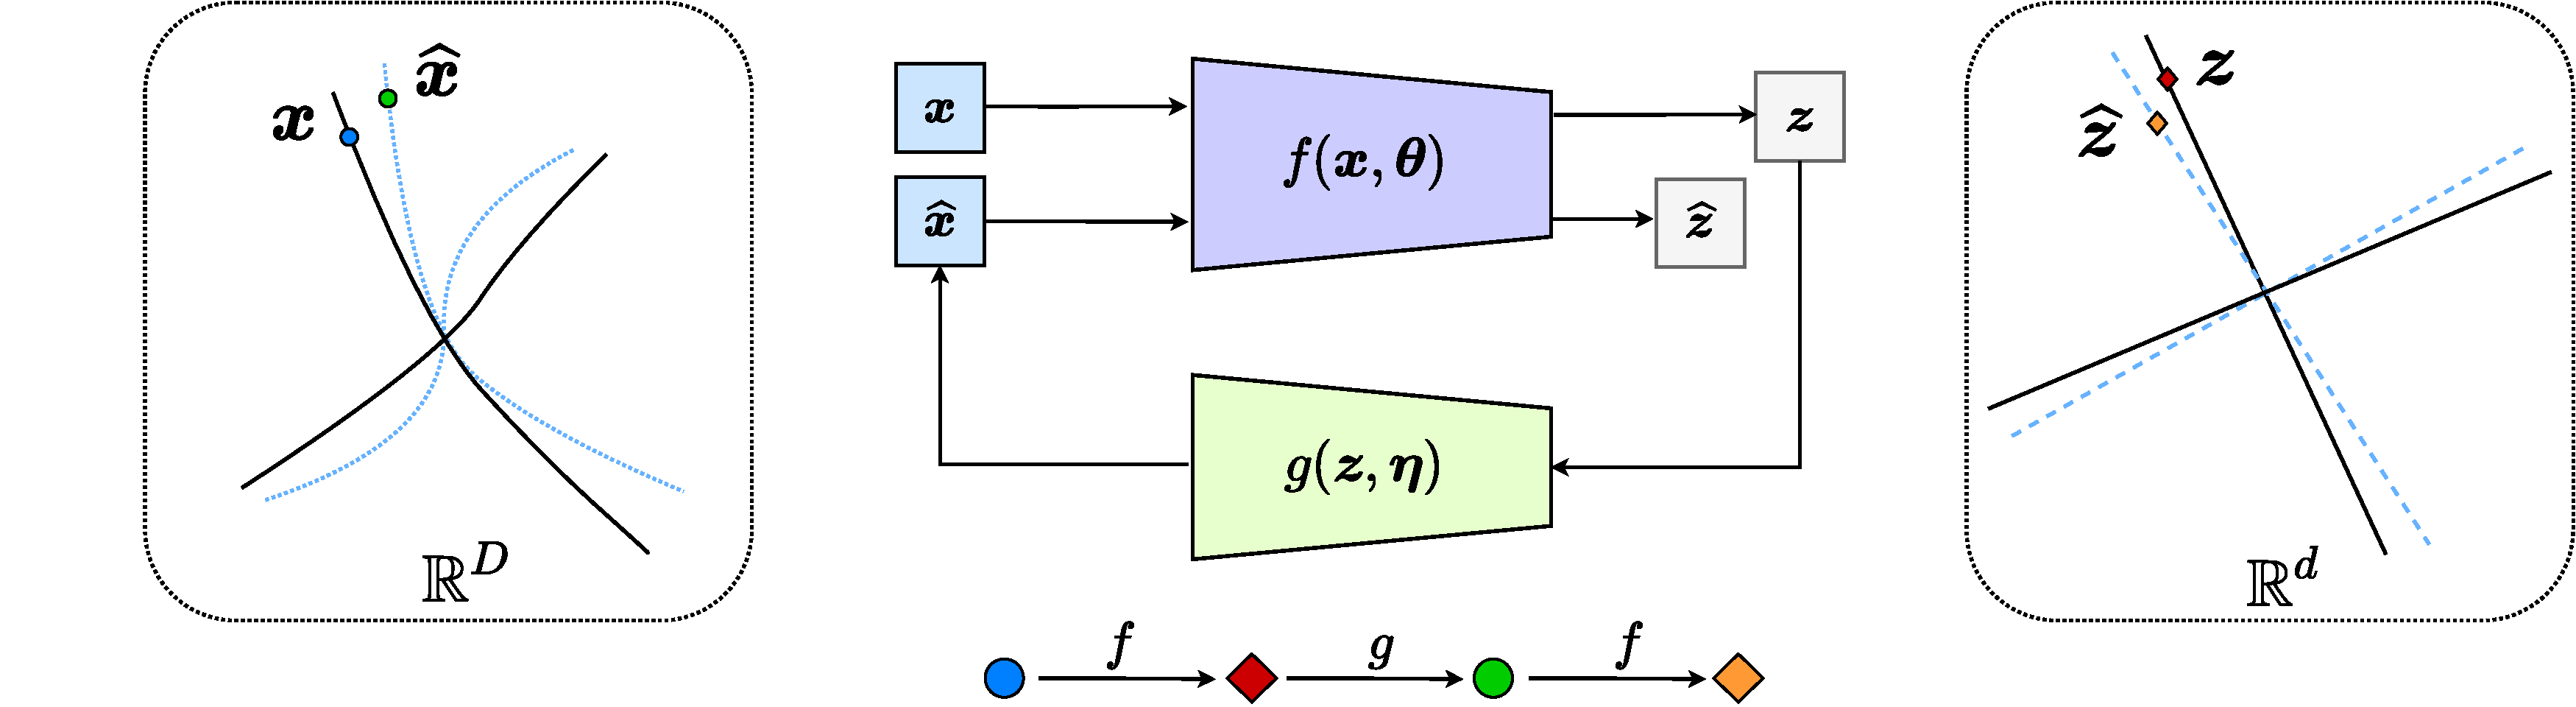
\includegraphics[width=0.9\linewidth]{\toplevelprefix/chapters/chapter1/figs/diagrams_redu_gan_2.pdf}}
\caption{一个闭环转录的图示。这里我们用映射 $f$ 来表示编码器 $\mathcal{E}$,用 $g$ 来表示解码器 $\mathcal{D}$。}  \label{fig:closed-loop}
\end{figure}

可以说,任何自主智能体只需要学习观测数据 $\X$ 的一个自洽表示 $\Z$,因为在原始数据空间(通常意味着在外部世界)中检查一致性要么太昂贵,要么甚至物理上不可行。闭环公式允许人们通过一个仅依赖于内部(学习到的)特征 $\Z$ 的极小极大博弈来学习一个最优的编码 $f(\cdot, \theta)$ 和解码 $g(\cdot, \eta)$:
\begin{equation}
\max_{\theta}\min_{\eta} \ell( \Z, \hat \Z) + \rho(\Z), 
   \label{eqn:closed-loop-objective}
\end{equation}
其中 $\ell( \Z, \hat \Z)$ 是一个基于特征 $\Z$ 和 $\hat \Z$ 编码率的损失函数,正如我们将看到的,它可以更容易计算。这里再次,$\rho(\Z)$ 是某个促进 $\Z$ 的简约性和信息丰富性的度量。有些令人惊讶的是,正如我们将在第\ref{ch:closed-loop}章中看到的,在相当温和的条件下,例如 $\X$ 是足够低维的,$(\Z, \hat \Z)$ 之间的自洽性意味着 $(\X, \hat \X)$ 的一致性!此外,我们还将看到,一个闭环系统将允许我们以一种{\em 连续和增量}的方式学习分布,\footnote{也就是说,一次学习一个类别,甚至一次学习一个样本。} 而不会遭受与开环模型相关的诸如灾难性遗忘等问题。

\section{连接机器智能的理论与实践}
到目前为止,我们已经介绍了三个相关的框架,用于学习给定数据分布 $\X$ 的一个紧凑且结构化的表示 $\Z$:
\begin{itemize}
\item 开环编码 \eqref{eqn:open-loop};
\item 双向自编码 \eqref{eqn:auto-encoding};
\item 闭环转录 \eqref{eqn:closed-loop}。
\end{itemize}
在本书中,我们将系统地研究所有这三个框架,一个接一个地:
\begin{equation}
    \mbox{\textbf{开环}} \; \Longrightarrow \; 
    \mbox{\textbf{双向}} \;  \Longrightarrow \; \mbox{\textbf{闭环}},
\end{equation}
分别在第\ref{ch:representation}章、第\ref{ch:consistent}章和第\ref{ch:closed-loop}章中。

在过去几年中,已经提出了许多理论框架来帮助理解深度网络。然而,许多框架未能提供与经验方法在真实世界数据和任务上的性能相匹配的可扩展解决方案。许多理论没有为如何进一步改进实践提供有用的指导。第\ref{ch:applications}章将展示本书提出的框架如何帮助弥合理论与实践之间的差距。我们将提供有说服力的实验证据,表明从第一性原理设计的网络和系统可以在各种任务上实现有竞争力的、甚至可能更好的性能,例如视觉表示学习、图像分类、补全、分割和文本生成。


\paragraph{回归智能。}
正如我们在开头提到的,任何智能体的基本任务都是从其感知的数据中学习可预测的信息。现在我们对这个任务的计算性质有了一些了解,我们应该意识到这是一个永无止境的过程,原因如下:
\begin{itemize}
    \item 当前从数据中学到的知识,比如说编码和解码方案,永远不可能是最优的。如果预测新观测时仍然存在错误,智能应该有能力改进。
    \item 到目前为止观察到的数据尚未涵盖所有可预测的信息。智能应该能够认识到当前知识的不足,并有能力学习和获取新信息。
\end{itemize}

因此,智能{\em 不是}简单地预先收集所有数据并训练一个模型来记住数据中所有可预测的信息。相反,它是关于配备了能够不断改进当前知识并在需要时获取新信息的计算机制。也就是说,任何智能体或系统\footnote{一个动物、一个人类、一个智能机器人、科学界,甚至整个文明。}的一个基本特征是{\em 能够自主地持续改进或获取信息(或知识)}。从概念上讲,我们可以将智能与信息(或知识)之间的关系图示如下:
\begin{equation}
\operatorname{智能}(t) = \odv*{\operatorname{信息}}{t}(t), \qquad 
\operatorname{信息}(t)  = \int_0^t \operatorname{智能}(s) \odif{s}.
\end{equation}
我们相信,闭环框架是一个通用的机制,它通过反馈和博弈使自我改进和自我学习成为可能。自然界中所有的智能体或系统在所有层面和所有尺度上都利用闭环机制进行学习。它的普遍性启发了早期试图通过机器和计算机来建模和模仿动物智能的研究,特别是1940年代由诺伯特·维纳发起的控制论运动。我们希望这本书能帮助人们更好地理解智能背后的目标、原理和计算机制。它可能为未来更深入、更广泛的智能研究奠定理论基础,我们将在本书的结尾,即第\ref{ch:future}章中进行更多讨论。

\end{document}